\documentclass[a4paper,11pt]{report}

\usepackage{setspace}
\usepackage{caption}
\usepackage{amsmath,amssymb,amsthm}
\usepackage{ wasysym }
\usepackage{ stmaryrd }
\usepackage{ mathpartir }
\usepackage{bussproofs}
\usepackage{enumerate}
\usepackage{tikz-qtree}
\usetikzlibrary{positioning}
\usetikzlibrary{arrows.meta}
\usetikzlibrary{arrows,shapes,quotes}
\usepackage{stackengine}
\usepackage{footmisc}
\usepackage{wrapfig}
\usepackage[a4paper,top=3cm,bottom=3.8cm,left=3cm,right=3cm,headsep=20pt]{geometry}
\usepackage[toc,page]{appendix}
\usepackage{listings}
\lstset{
	language=bash,
	basicstyle=\ttfamily
}


\usepackage{hyperref}% http://ctan.org/pkg/hyperref
\usepackage{cleveref}% http://ctan.org/pkg/cleveref

\theoremstyle{definition}
\newtheorem{theorem}{Theorem}[section]
\theoremstyle{definition}
\newtheorem{corollary}[theorem]{Corollary}
\theoremstyle{definition}
\newtheorem{lemma}[theorem]{Lemma}
\theoremstyle{definition}
\newtheorem{proposition}[theorem]{Proposition}
\theoremstyle{definition}
\newtheorem{definition}[theorem]{Definition}
\theoremstyle{definition}
\newtheorem{example}[theorem]{Example}
\theoremstyle{definition}
\newtheorem{remark}[theorem]{Remark}
\begin{document}
	
	
	\pagenumbering{gobble}
	\newgeometry{top=2cm, right=2.5cm, left=2.5cm, bottom=2.5cm}
	\begin{flushright}
		% https://public.univie.ac.at/en/downloads/logos/
		\includegraphics[width=7cm]{RZ_Logo_Uni_sw}
	\end{flushright}	
	\vskip20mm
	\begin{center}
		\huge\textbf{MASTERARBEIT / MASTER'S THESIS}
		\vskip15mm
		\normalsize{Titel der Masterarbeit / Title of the Master's Thesis}
		
		\LARGE\textbf{``Automated Deduction for Intuitionistic Logic\\via Embedding into Classical Logic''} % Insert title here
		\vskip15mm
		\normalsize{verfasst von / submitted by}
		
		\Large\textbf{Alexander Pluska, BSc} % Insert your name in this line
		\vskip15mm
		\normalsize{angestrebter akademischer Grad / in partial fulfillment of the requirements for the degree of}
		
		\Large\textbf{Master of Science (MSc)}
		
		\small
	\end{center}
	\vskip15mm
	\begingroup
	\renewcommand{\arraystretch}{1.2}
	\begin{flushleft}
		Wien, 2022 / Vienna, 2022 % Insert graduation year in this line
		\vfill
		\addtolength{\tabcolsep}{-6pt} 
		\begin{table}[h!]
			\begingroup
			\renewcommand*{\arraystretch}{1.2}
			%\renewcommand*{\linespacing}{1}
			\renewcommand\baselinestretch{1}
			\small
			\begin{tabular}{p{7cm} p{10cm}}
				Studienkennzahl lt. Studienblatt / \newline degree programme code as it appears on \newline the student record sheet: &UA 066 821 \\
				Studienrichtung lt. Studienblatt / \newline degree programme as it appears on \newline the student record sheet:& Masterstudium Mathematik\\
				Betreut von / Supervisor: & Univ.-Prof. Matthias Aschenbrenner, PhD
			\end{tabular}
			\endgroup
		\end{table}
		\addtolength{\tabcolsep}{6pt} 
	\end{flushleft}	
	\endgroup	
	\restoregeometry
	
	\newpage
	\
	\newpage
	
	% Some of the code for creating ToC id adapted from the following template:
	% https://www.sharelatex.com/templates/thesis/university-of-sussex-thesis
		
		\
		\vfill
		\onehalfspacing
		\begin{center}
		\bfseries Abstract		
		\end{center}
		The famous double negation translation~\cite{glivenko1929quelques, godel1933intuitionistischen} establishes an embedding from classical into intuitionistic logic. Curiously, the reverse direction has not been covered in literature. We present an effective embedding from intuitionistic into classical logic, both in the propositional and first-order case, as well as an effective embedding of intuitionistic propositional logic into quantified boolean formulas.
		
		Furthermore, we implement a system that takes intuitionistic first-order problems in the tptp file format as an input and performs our transformation. This allows the use of classical theorem provers for checking intuitionistic validity. We benchmark our implementation using the Vampire theorem prover~\cite{kovacs2013first} on the ILTP problem set~\cite{iltp}.
		
		Finally, we discuss how the generated classical proofs of the transformed problem can be translated back into intuitionistic proofs of the original problem. All in all, this establishes a novel approach to theorem proving for intuitionistic logic and provides a first proof of concept.

	\vspace*{1cm}
	\begin{center}
		\bfseries Acknowledgements		
	\end{center}
	
	I want to thank Matthias for accommodating my particular interests by agreeing to supervise a thesis which lies outside his main area of research and bearing with the organizational difficulties.
	
	I sincerely appreciate Florian's guidance, who graciously agreed to co-supervise a thesis at a different university. He has provided me with a fascinating topic as well as plenty of his time, expertise and thorough feedback.
	
	Finally, I am incredibly grateful to my family, in particular my parents Stefania and Cezary, who have instilled in me the joy of learning, provided all the love and help I could ask for and invariably supported me along my journey.
	
	{\vfill\null}
	
	\newpage
	\
	\singlespacing
	\newgeometry{top=1cm, bottom=2cm}
	\tableofcontents
	\restoregeometry

	\chapter{Introduction}
	\onehalfspacing


	\pagenumbering{arabic}
	Constructive mathematics refers to a flavour of mathematics in which the existence of an object can only be established by explicit construction, as opposed to classical mathematics where existence can be shown implicitly, e.g. by assuming non-existence and deriving a contradiction.
	The formalism usually associated with constructive mathematics is intuitionistic logic, which essentially differentiates itself from classical logic by the fact that the law of excluded middle $A\vee\neg A$ and the double negation shift $\forall x\neg\neg P(x)\to\neg\neg\forall xP(x)$ are not valid.
	Besides philosophical considerations, most prominently advocated by Brouwer~\cite{brouwer1907over} and Bishop~\cite{bishop1967foundations}, there is a particular motivation for studying constructive mathematics from the perspective of computer science in that proofs in  intuitionistic logic directly correspond to computer programs --- as expressed in the Curry-Howard correspondence~\cite{howard1980formulae}.
	
	The interest in intuitionistic logic has led to the development of a number of automated theorem proving systems for propositional as well as for predicate logic and a collection of benchmark problems (see e.g. the
	ILTP library website~\cite{iltp}).
	However, progress in automated theorem proving for intuitionistic logic has been slow, whereas reasoners for classical logic have made tremendous progress, see e.g. the TPTP~\cite{casc} and SAT~\cite{satc} competitions.
	This difference can be partially explained by fundamental differences between the logics.
	Foremost, determining intuitionistic validity is computationally harder, i.e. in the propositional case intuitionistic validity is \verb+PSPACE+-complete~\cite{statman1979intuitionistic} whereas classical validity is \verb+coNP+-complete~\cite{cook1971complexity}.
	A further advantage of classical logic is the existence of calculi that are particularly suitable for automation such as superposition~\cite{bachmair2001resolution}, which rely on the existence of convenient normal forms such as CNF, and the duality between validity and satisfiability, i.e. to show the validity of a formula it suffices to show the unsatisfiability of the negated formula.
	While some (albeit more complex) normal forms also exist  for intuitionistic logic, crucially the duality between validity and satisfiability of the negation does not hold.
	Therefore, most dedicated intuitionistic theorem provers~\cite{mclaughlin2009efficient, tammet1996resolution} use the naive inverse method, i.e. direct search for a cut-free proof by applying the rules from some proof calculus inversely, enhanced by search strategies such as focussing and polarization. This approach generally leads to a much more complex search and is therefore difficult to implement efficiently.
	Finally, we add that in contrast to intuitionistic provers a tremendous amount of work has been put into optimizing provers for classical logic, in particular for the propositional case, i.e. SAT-solvers.
	
	With this work we want to propose a novel approach for intuitionistic theorem proving that leverages the progress in classical theorem proving, that is for each formula $\varphi$:
	\begin{itemize}
		\item Give a formula $\varphi^\#$ that is classically valid if and only if $\varphi$ is intuitionistically valid.
		\item Use a state-of-the-art classical prover to establish the validity/invalidity of $\varphi^\#$.
		\item Transform the generated proof/counter-model of $\varphi^\#$ to one of $\varphi$.
	\end{itemize}
	The most challenging part of this approach is giving the translation of $\varphi$ to $\varphi^\#$.
	Interestingly, the reverse direction, the famous double-negation translation, has long been established and goes back to Glivenko~\cite{glivenko1929quelques} in the propositional case, and to G\"odel~\cite{godel1933intuitionistischen} and Gentzen~\cite{gentzen1936widerspruchsfreiheit} in the first-order case. In the propositional case, it is particularly simple: $\varphi$ is classically valid if and only if $\neg\neg\varphi$ is intuitionistically valid. Intuitively, the translation collapses for each subformula $\psi$ of $\varphi$ the truth values of $\psi$ and $\neg\neg\psi$, which are classically but not intuitionistically equivalent. This gives us a first idea why the reverse direction is perhaps more difficult: We need to expand the truth values of $\psi$ and $\neg\neg\psi$, i.e. if they both occur in $\varphi$, we must have a way to (classically) assign different truth values to their respective counterparts in $\varphi^\#$. In particular, this necessitates the introduction of new propositional variables in our procedure, which already marks a big difference to the double negation translation.
	
	While establishing the translation of formulas we also perform an effective translation of counter-models, i.e. for each intuitionistic counter-model of $\varphi$ we effectively construct a classical counter-model of $\varphi^\#$ and vice versa.
	We note that the existence of counter-models is a key notion that forms a proper dual to validity --- whereas the satisfiability of the negation is not necessary for invalidity (in contrast to classical logic, where it is a proper dual to validity).
	Transforming and reducing counter-models to a normal form is also what ultimately enables our translation. Apart from a translation of counter-models in the final chapter, we also explicitly describe how to equivalently transform classical proofs of $\varphi^\#$ to intuitionistic proofs of $\varphi$.
	
	
	As a final contribution, we implement our translation in the Rust programming language. Our implementation transforms a first-order problem in the tptp format~\cite{tptp} and outputs the translated problem in the same format. The code is published on GitHub~\cite{implementation}. We then benchmark our implementation using the ILTP problem set~\cite{iltp}, i.e. we translate all problems in the set and then run the Vampire theorem prover~\cite{Kov_cs_2013} on the translated problems. Our approach performs on par with existing approaches for intuitionistic theorem proving, but comes short of the state-of-the art. As there is still a lot of room for optimization, this is a hopeful first sign.
	
	\chapter{Overview}

	The main content is organized in chapters 3 to 6. Chapter 3 collects prerequisite definitions and serves to fix our notation and recall some important facts. Chapter 4 is the meat of this thesis. In particular, it features a complete description of our embedding of intuitionistic into classical logic as well as proving its correctness. In chapter 5 we present the implementation of the embedding and the results of our benchmark. Finally, in chapter 6 we explicitly describe how to translate the generated proofs and counter-models which in principle directly follows from the results of section 4. 	We shall now for each chapter give an overview of our main results and highlight the key arguments. 

	\section{Embedding intuitionistic into classical logic}

	Recall that our goal in this chapter is to give an effective translation procedure that, for a given formula $\varphi$, yields a formula $\varphi^\#$, such that $\varphi$ is intuitionistically valid if and only if $\varphi^\#$ is classically valid. We start with the propositional case. The key arguments are the same as in the first-order case, while it is technically simpler and less cluttered.
	
	Before our main transformation we employ a preprocessing step akin to the Tseytin transformation~\cite{tseitin1983complexity}, which is a popular pre-processing step in classical automated reasoning:
	It gives an equisatisfiable sentence (over an extended set of propositions) in conjunctive normal form.
	Eliminating all implications, however, is not possible in intuitionistic logic since $A\to B$ is not equivalent to $\neg A\vee B$.
	Still, we propose a similar transformation.
	A notable feature of our transformation is that all non-classical content is encapsulated in formulas of type $(A\to B)\to C$, i.e. if there are no such formulas in the transformed formula then the classical validity of the transformed formula immediately implies intuitionistic validity and no further processing is needed.
	
	\begin{theorem}\label{thm:Tseytin1}
		For every propositional formula $\varphi$ there effectively are an atom $P$ and a set of $\mathcal S$ of formulas (over an extended set of propositions) of one of the forms\\
		$\text{ \hspace{1cm}} A\to (B\wedge C), (A\wedge B)\to C, A\to (B\vee C), (A\vee B)\to C, (A\to B)\to C,$\\
		for atomic $A, B, C$, such that $\varphi$ is intuitionistically valid if and only if $\bigwedge\mathcal S\to P$ is intuitionistically valid. The time complexity of the transformation is linear in the input size.
	\end{theorem}
	
	The main transformation then proceeds in three steps:
	%
	1) We encode as a first-order sentence that the considered formula holds for every Kripke frame.
	Since Kripke frames for propositional logic over a fixed alphabet of propositional variables form a first-order theory, this step is rather straightforward.
	%
	2) Next we eliminate some quantifiers via Herbrandization. The only quantifiers eliminated occur in formulas derived from formulas of type $(A\to B)\to C$.
	%
	3) We can then argue that if there is a counter-model for the resulting formula, then there is a counter-model with a certain Kripke frame of bounded size completely determined by the number of formulas of type $(A\to B)\to C$.
	This allows us to eliminate the remaining quantifiers by simply enumerating the worlds in that Kripke frame.
	
	Summarizing, we obtain the following result:
	
	\begin{theorem}
		\label{thm:reduction-propositional}
		Let $\mathcal S$ be as in Theorem~\ref{thm:Tseytin1} and $\mathcal F_\to\subseteq\mathcal S$ denote the subset of formulas of the form $(A\to B)\to C$ and $\Lambda$ denote the set of sequences without repetition over $\mathcal F_\to$. For each atom $A$ and $k\in\Lambda$ consider a new atom $A^k$. Obtain $\mathcal S^\#$ by including the following formulas:
		\begin{itemize}
			\item $A^k\to A^{k\psi}$ for each atom $A$ occurring in $\mathcal S$, $k\in\Lambda$ and $\psi\in\mathcal F_\to$ not occurring in $k$.
			\item $A^k\to (B^k\circ C^k)$ for each $\circ\in\{\wedge,\vee\}$, $A\to (B\circ C)\in\mathcal S$, $k\in\Lambda$.
			\item $(A^k\circ B^k)\to C^k$ for each $\circ\in\{\wedge,\vee\}$, $A\to (B\circ C)\in\mathcal S$, $k\in\Lambda$.
			\item $(A^{k\psi}\to B^{k\psi})\to C^k$ for $\psi = (A\to B)\to C\in\mathcal S$, $k\in\Lambda$ if $\psi$ does not occur in $k$.
		\end{itemize}
		Then, $\bigwedge S\to P$ is intuitionistically valid iff $\bigwedge S^\#\to P^\epsilon$ is classically valid, where $\epsilon$ denotes the empty sequence. The size of $\mathcal S^\#$ is in $\mathcal O(|\mathcal S|\cdot2^{|\mathcal F_\to|\cdot\log(|\mathcal F_\to|)})$. Furthermore, there is an effective procedure for translating counter-models between the sentences.
	\end{theorem}
	
	Instead of explicitly enumerating the worlds of a counter-example of bounded size (as in the reduction stated in the above theorem), we can also do this enumeration implicitly with a quantified boolean formula (QBF).
	We can show that this QBF is satisfiable iff there exists a counter-model for our original formula:
	
	\begin{theorem}
		Let $\mathcal S$ be as in Theorem~\ref{thm:Tseytin} and $\mathcal F_\to\subseteq\mathcal S$ denote the subset of formulas of the form $(A\to B)\to C$. There is an effective procedure that produces a QBF $\varphi^Q$ of size $\mathcal O(|\mathcal S|\cdot|\mathcal F_\to| + |\mathcal F_\to|^3)$ with $2\cdot |\mathcal F_\to|-1$ quantifier alternations such that $\varphi$ is intuitionistically valid if and only if $\varphi^Q$ is not satisfiable. For fixed $N\in\mathbb N$, deciding intuitionistic validity for formulas $\bigwedge \mathcal S\to P$ where $\mathcal S$ is as above and $|\mathcal F_\to| = N$ is therefore in $\Sigma_{2N-1}$.
	\end{theorem}
	
	We then move to the first-order case. Here the construction is a bit more involved, but the underlying approach is the same.
	Again, we first perform a Tseytin-like transformation.
	Here the non-classical content is encapsulated by formulas of type $(A\to B)\to C$ and $\forall xA\to B$.
	The details of this translation are given in Section~\ref{section:tseytin}.
	We then proceed similarly to the propositional case.
	Note however that one difficulty arises from the fact that our (classical) domain will now contain on the one hand worlds in the Kripke frame, but on the other hand also proper domain elements.
	We resolve this apparent conflict by introducing a special binary predicate $E$, inspired by~\cite{iemhoff2010eskolemization}, encoding which domain elements exists at which world.
	The main transformation then again proceeds in three steps:
	Step 1) and 2) are analogous to the propositional case.
	The real difference arises in step 3):
	While we can also establish the existence of a canonic counter-model whose frame only depends on formulas of type $(A\to B)\to C$ and $\forall xA\to B$, the size of this counter-model is countably infinite in general.
	This is not surprising, since certain intuitionistically invalid formulas like the double negation shift $\forall x\neg\neg A(x)\to \neg\neg\forall x A(x)$ don't have finite counter-models.
	Therefore, we are not able to eliminate the $\forall$-quantifiers associated with the Kripke semantics.
	However, since our translation targets first-order logic, we believe that the introduction of these quantifiers is acceptable.
	
	Summarizing, we obtain the following result:
	
	\begin{theorem}
		\label{thm:reduction-first-order-short}
		There exists a linear-time procedure that gives for every first-order formula $\varphi$ a formula $\varphi^\#$ such that $\varphi$ is intuitionistically valid if and only if $\varphi^\#$ is classically valid. The size of $\varphi^\#$ is in linear in the size of $\varphi$, however, for each $n$-ary relation symbol in $\varphi$ there is a corresponding $n+1$-ary relation symbol in $\varphi^\#$, and $\varphi$ contains a new binary predicate $E$ as well as a number of new function symbols. Furthermore, there is an effective translation between intuitionistic counter-models of $\varphi$ and classical counter-models of $\varphi^\#$.
	\end{theorem}
	A more detailed account of Theorem~\ref{thm:reduction-first-order-short} is given in Theorem~\ref{fullFOtranslation}.
	
	\section{Implementation}
	
	In this section, we describe our system that implements the translation from the previous section. The rust source code can be found online~\cite{implementation}. We then elaborate our benchmarking process, which utilizes the ILTP problem set~\cite{iltp} and the Vampire theorem prover~\cite{Kov_cs_2013}.
	
		
	\begin{figure}[h]\label{results}
		$$\begin{matrix}
			&\text{AGT}&\text{ALG}&\text{COM}&\text{CSR}&\text{GEJ}&\text{GEO}&\text{GPJ}&\text{GRA}\\
			\text{Proven}&5&170&0&0&58&3&4&2\\
			\text{Disproven}&0&0&0&0&0&0&0&0\\
			\text{Timeout}&47&29&3&29&107&74&1&16
		\end{matrix}$$
		$$\begin{matrix}
			&\text{GRP}&\text{HAL}&\text{KRS}&\text{LCL}&\text{MGT}&\text{MSC}&\text{NLP}&\text{NUM}\\
			\text{Proven}&0&0&30&1&9&1&9&2\\
			\text{Disproven}&0&0&0&0&12&0&0&0\\
			\text{Timeout}&5&9&128&3&69&1&237&82
		\end{matrix}$$
		$$\begin{matrix}
			&\text{PLA}&\text{PUZ}&\text{SET}&\text{SWC}&\text{SWV}&\text{SYJ}&\text{SYN}&\text{TOP}\\
			\text{Proven}&0&5&27&1&64&65&54&1\\
			\text{Disproven}&0&1&0&0&2&3&13&0\\
			\text{Timeout}&6&1&297&422&154&108&298&2
		\end{matrix}$$
		\caption{Performance on problem sections of the ILTP set.}
	\end{figure}
	
	Our implementation performs similar to existing dedicated provers for intuitionistic logic, but falls short of the state-of-the-art. Since there is still a lot of possible optimizations left for our translation, this is a hopeful first sign.
	
	\section{Translation of counter-models and proofs}
	
	In the final section, we give an explicit mechanism how to transform the proofs and counter-models for translated formula $\varphi^\#$ into intuitionistic proofs/counter-models of the original formula $\varphi$. The existence of these transformations is clear from the methodology of chapter~\ref{chapter:eiicl}, however, they are hidden in the proofs and here we make them explicit. The two main results are as follows:
	\begin{theorem}
		There exists an effective procedure that converts any classical counter-model for a translated formula $\varphi^\#$ into an intuitionistic counter-model for the original formula $\varphi$.
	\end{theorem}
	\begin{theorem}
		There exists an effective procedure that converts any classical proof of a translated formula $\varphi^\#$ into a intuitionistic proof of the original formula $\varphi$.
	\end{theorem}
	
	Given the arguments of Chapter~\ref{chapter:eiicl} the translation of counter-models is more or less just a compilation of proofs. On the other hand, the explicit translation of proofs does require some work, since to that point all arguments were semantic and this requires a syntactic viewpoint.

	\chapter{Preliminaries}
	First, let us recapitulate the most important definitions and some facts about them. This will serve to fix our notation as well.
	
	\section{Syntax}
	
	\subsection{Propositional logic}
	
	Let us fix some countably infinite set of propositional variables $A, B, C\dots$.
	
	\begin{definition}
		A \textit{formula} and \textit{subformula} is defined inductively via the following rules:
		\begin{itemize}
			\item every propositional variable as well as a special symbol $\bot$ is a formula, such a formula is called \textit{atomic} and $A,B,C,\dots$ and $\bot$ are called \textit{atoms}.
			\item if $\varphi$ and $\psi$ are formulas then $\varphi\circ\psi$ is a formula for $\circ\in\{\wedge,\vee,\to\}$.
			\item every formula is a subformula of itself.
			\item for a formula $\chi = \varphi\circ\psi$ every subformula of $\varphi$ and $\psi$ is also a subformula of $\chi$.
		\end{itemize}
	We write $\neg \varphi$ for $\varphi\to \bot$.
	\end{definition}

	\subsection{Predicate logic}
	
	The analogon for predicate logic is much more involved as we need to define terms.
	
	\begin{definition}
		A \textit{signature} consists of
		\begin{itemize}
			\item a finite set $S_f$ of function symbols $f_1, \dots, f_n$
			\item a finite set $S_R$ of relation symbols $R_1,\dots, R_m$
			\item  a function ar$: S_f\cup S_R\to \mathbb{N}$ assigning to each symbol its arity (possibly 0). 
		\end{itemize}
	\end{definition}
	
	\noindent Usually the signature will be left implicit. If explicitly stated we denote it by $$\{f_1/\text{ar}(f_1),\dots,f_n/\text{ar}(f_n), R_1/\text{ar}(R_1).\dots,R_m/\text{ar}(R_m)\}.$$
	Fix a countably infinite collection of free variables $a, b, c\dots$ and bound variables $x, y, z\dots$.
	Note that the following definitions could be simplified by not distinguishing between bound and free variables. However, this has some other drawbacks and in particular when defining a sequent calculus for first-order logic having disjoint sets of bound and free variables is convenient.
	
	\begin{definition}
		A \textit{semiterm} is defined inductively via the following rules
		\begin{itemize}
			\item each variable is a term
			\item if $t_1,\dots,t_n$ are terms and $f$ a $n$-ary function symbol then $f(t_1, \dots, t_n)$ is a term.
		\end{itemize}
		A \textit{term} is a semiterm in which each occurring variable is a free variable. Every term is a semiterm. Analogously to the definition of subformulas we can define \textit{subsemiterms} and \textit{subterms}.
	\end{definition}

	\begin{definition}
		A \textit{Substitution} is a function $\sigma$ from free variables to semiterms. For a semiterm $t$ we define $t\sigma$ as follows:
		\begin{itemize}
			\item $x\sigma = x$ if $x$ is bound.
			\item $a\sigma = \sigma(a)$ if $a$ is free.
			\item $f(t_1,\dots,t_n)\sigma = f(t_1\sigma,\dots,t_n\sigma)$.
		\end{itemize}
	\end{definition}
	
	\begin{definition}
		A \textit{formula} is defined inductively via the following rules
		\begin{itemize}
			\item $\bot$ is a formula.
			\item if $t_1,\dots,t_n$ are terms and $R$ and an $n$-ary relation symbol then $R(t_1, \dots, t_n)$ is a formula.
			\item if $s, t$ are terms then $s = t$ is a formula.
		\end{itemize}	
		Formulas formed by the above rules are called \textit{atomic}.
		\begin{itemize}
			\item If $\varphi$ and $\psi$ are formulas then $\varphi\circ\psi$ is a formula for $\circ\in\{\wedge,\vee,\to\}$.
			\item If $\varphi$ is a formula and $a$ is a free variable occurring in $\varphi$ and $x$ is a bound variable not occurring in $\varphi$ then $Qx(\varphi[x/a])$ is a formula for $Q\in\{\exists,\forall\}$ where the \textit{substitution} $\varphi\sigma$ is defined inductively via
			\begin{itemize}
				\item $\bot\sigma = \bot$
				\item $R(t_1,\dots,t_n)\sigma = R(t_1\sigma,\dots, t_n\sigma)$
				\item $(s = t)\sigma = (s\sigma = t\sigma)$
				\item $(\varphi\circ\psi)\sigma = \varphi\sigma\circ\psi\sigma$ for $\circ\in\{\wedge,\vee,\to\}$.
				\item $(Qy\varphi)\sigma = Qy(\varphi\sigma)$ for $Q\in\{\exists,\forall\}$.
			\end{itemize}
			\item A formula containing no free variables is a \textit{sentence}.
		\end{itemize}
	\end{definition}

	\section{Semantics}
	
	Classical and intuitionistic semantics give (different) meaning to formulas.
	
	\subsection{Propositional Logic}
	\subsubsection{Classical Semantics}
	
	\begin{definition}
		A \textit{valuation} $v$ is a function that assigns to each propositional variable $A$ a \textit{truth value} $v(A)\in\{0, 1\}$. We define a model relation $\models$ between valuations $v$ and formulas:
		\begin{itemize}
			\item $v\not\models \bot$
			\item $v\models A$ iff $v(A) = 1$ for each propositional variable $A$.
			\item $v\models \varphi\wedge\psi$ iff $v\models\varphi$ and $v\models\psi$.
			\item $v\models\varphi\vee\psi$ iff $v\models\varphi$ or $v\models\psi$.
			\item $v\models\varphi\to \psi$ iff $v\not\models\varphi$ or $v\models\psi$.
		\end{itemize}
		$v$ is a \textit{model} for $\varphi$ if $v\models\varphi$. $\varphi$ is \textit{satisfiable} if there exists a valuation which is a model. It is \textit{valid} if every valuation is a model, and we write $\models \varphi$. We denote the set of valid formulas with CPC. We can furthermore define an entailment relation between sets of clauses, that is $\mathcal S\models_C \mathcal T$ if for every valuation $v$ with $v\models\bigwedge S$ we have $v\models\bigvee \mathcal T$.
	\end{definition}
	
	One notable property of classical logic is that a formula $\varphi$ is valid iff its negation, i.e. $\neg\varphi$ is not satisfiable. The same does not hold true for intuitionistic logic, as we shall see.

	\subsubsection{Intuitionistic Semantics}
	
	\begin{definition}
		A \textit{Kripke structure} $\mathcal K = (W, (v_w)_{w\in W})$ consists of a partially ordered set $W$ of nodes an a family of valuations $(v_w)_{w\in W}$ such that for $u\leq w$ we have $v_u(A)\leq v_u(A)$ for every propositional variable $A$, this is called the \textit{persistency condition}. In this case, we define a model relation between worlds $u$ and formulas. It is slightly different in the case of implications, i.e. have
		\begin{itemize}
			\item $u\not\models \bot$
			\item $u\models A$ iff $v_u(A) = 1$ for each propositional variable $A$.
			\item $u\models \varphi\wedge\psi$ iff $v\models\varphi$ and $v\models\psi$.
			\item $u\models\varphi\vee\psi$ iff $v\models\varphi$ or $v\models\psi$.
			\item $u\models\varphi\to \psi$ if for all $w\geq u$ we have $w\not\models\varphi$ or $w\models\psi$.
		\end{itemize}
		We say that $\varphi$ is satisfied at a node $u$ if $u\models\varphi$. If a formula is satisfied at every node, then $K$ is a \textit{model} for $\varphi$, and we write $K\models \varphi$. $\varphi$ is satisfiable if there exists a Kripke structure, which is a model. It is \textit{valid} if every Kripke structure is a model and we write $\models \varphi$. We denote the set of valid formulas with IPC. As before, we define an entailment relation $\models_I$ between sets of formulas.
	\end{definition}
	There are many classical tautologies which are not intuitionistically valid
	\begin{example}\label{LEMcounterexample}
		Consider the famous law of excluded middle $A\vee\neg A$. As a counter model consider a Kripke structure with two nodes $u\leq w$ and $v_u(A) = 0, v_w(A) = 1$. Then $u\not\models A$ and $u\not\models \neg A$, i.e. $u\not\models A\vee\neg A$. 
	\end{example}
	The following is a famous and important result due to Glivenko~\cite{glivenko1929}
	
	\begin{theorem}[Glivenko's theorem]
		A propositional formula $\varphi$ is classically valid iff $\neg\neg\varphi$ is intuitionistically valid.
	\end{theorem}
	\noindent Note however that this difference between classical and intuitionistic logic is not reflected in satisfiability, only in validity:
	\begin{lemma}\label{propsat}
		A propositional formula $\varphi$ is intuitionistically satisfiable if and only if it is classically satisfiable.
	\end{lemma}

	\begin{proof}
		Every classical model can be viewed as a Kripke model with a single node. Therefore, classical satisfiability trivially implies intuitionistic satisfiability.	On the other hand, in every Kripke structure that is a model every node is a classical model so intuitionistic satisfiability implies intuitionistic satisfiability.
	\end{proof}

	In classical logic, a proven strategy for showing that a formula valid is to consider its negation and show that it is not satisfiable. Due to the previous lemma, this is insufficient for intuitionistic logic. There are formulas like $A\vee\neg A$ which are not an intuitionistic tautology, while their negation is not satisfiable either. This serves to motivate the consideration of equivalidity in the following chapters. In the context of classical logic it can be fully explained via equisatisfiability and is therefore neglected, but for intuitionistic logic it is more fundamental.
	
	Finally, let us note the complexities of these various decision problems, which play a fundamental role in all of theoretical computer science.
	
	\begin{theorem}
		Satisfiability for classical and intuitionistic propositional logic is \verb+NP+-complete.
	\end{theorem}

	For classical logic this is the famous Cook-Levin theorem first published in Cook's seminal paper~\cite{cook1971complexity}. Of course, we have seen that the intuitionistic case is the same decision problem.
	
	\begin{corollary}
		Validity for classical logic is \verb+co-NP+-complete
	\end{corollary}

	This is clear, since validity is just the complementary problem to satisfiability of the negated formula. However, in intuitionistic logic unfortunately validity is really harder than satisfiability as first shown by Statman~\cite{statman1979intuitionistic}.
	
	\begin{theorem}
		Validity for intuitionistic logic in \verb+PSPACE+-complete.
	\end{theorem}

	One thing to note is that in contrast to predicate logic, all these problems are decidable.
	
	
	\subsection{Predicate Logic}

	We now give account of the more involved semantics of first-order logic
	
	\subsubsection{Classical Semantics}

	\begin{definition}
		Let $\Sigma$ be a signature. A $\Sigma$-structure $\mathcal{M}$ consists of a non-empty set $M$, the domain of $\mathcal{M}$, and a function $I$ that assigns
		\begin{itemize}
			\item to each $n$-ary function symbol $f$ a $n$-ary function $f^I: M^n\to M$.
			\item to each $n$-ary relation symbol $R$ a $n$-ary relation $R^I\subseteq M^n$.
		\end{itemize}
		A variable assignment $v$ is a function that assigns to each free variable an element $m\in M$. For each free variable $a$ and $m\in M$ we define $$v[m/a](b) = \begin{cases}
			m&\text{if $b=a$}\\
			v(b)&\text{otherwise}
		\end{cases}$$
		Then terms are interpreted as follows:
		\begin{itemize}
			\item $a^{I, v} = v(a)$ for each free variable $a$.
			\item $f(t_1,\dots,t_n)^{I, v} = f^I(t_1^{I, v},\dots, t_n^{I, v})$.
		\end{itemize}
		We define a model relation between pairs $\mathcal M, v$ and formulas $\varphi$ as follows
		\begin{itemize}
			\item $\mathcal M, v\not\models\bot$.
			\item $\mathcal M, v\models R(t_1,\dots,t_n)$ iff $(t_1^{I, v},\dots,t_n^{I, v})\in R^I$.
			\item $\mathcal M, v\models s = t$ iff $s^{I, v} = t^{I, v}$.
			\item $\mathcal M, v\models \varphi\wedge \psi$ iff $\mathcal M, v\models\varphi$ and $\mathcal M, v\models\psi$.
			\item $\mathcal M, v\models \varphi\vee\psi$ iff $\mathcal M, v\models\varphi$ or $\mathcal M, v\models\psi$.
			\item $\mathcal M, v\models \varphi\to\psi$ iff $\mathcal M, v\not\models\varphi$ or $\mathcal M, v\models\psi$.
			\item $\mathcal M, v\models\exists x\varphi$ iff there exists $m\in M$ such that $\mathcal M, v[m/a]\models\varphi[a/x]$ where a is a free variable that does not occur in $\varphi$.
			\item $\mathcal M, v\models\forall x\varphi$ iff for all $m\in M$ we have $\mathcal M, v[m/a]\models\varphi[a/x]$ where a is a free variable that does not occur in $\varphi$.
		\end{itemize}
		$\varphi$ is satisfiable if for some $\mathcal{M}, v$ we have  $\mathcal M, v\models\varphi$. It is valid if for all  $\mathcal M, v$ we have  $\mathcal M, v\models\varphi$. We write $\mathcal{M}\models\varphi$ if for every $v$ we have  $\mathcal M, v\models\varphi$. We denote the set of valid formulas with CQC. As before define an entailment relation $\models_C$ between sets of formulas.
	\end{definition}

	\subsubsection{Intuitionistic Semantics}
	
	\begin{definition}
		A $\Sigma$-\textit{Kripke structure} $\mathcal{K}$ is a partially ordered set $W$ and a family of $\Sigma$-structures $(\mathcal{M}_w)_{w\in W}$ such that for $u\leq w$
		\begin{itemize}
			\item $M_u\subseteq M_w$.
			\item $f^{I_w}|_{M_u} = f^{I_u}$.\footnote{Here $f|_M$ denotes the restriction of $f$ to $M$.}
			\item $R^{I_w}|_{M_u} = R^{I_u}$.
		\end{itemize}
		Then we define a model relation between worlds $u\in W$ and variable assignments $v$ (targeting $M_u$) and formulas $\varphi$ as follows:
		\begin{itemize}
			\item $u, v\not\models\bot$
			\item $u, v\models R(t_1,\dots,t_n)$ iff $(t_1^{I_u, v},\dots,t_n^{I_u, v})\in R^{I_u}$.
			\item $u, v\models s = t$ iff $s^{I_u, v} = t^{I_u, v}$.
			\item $u, v\models \varphi\wedge \psi$ iff $u, v\models\varphi$ and $u, v\models\psi$.
			\item $u, v\models \varphi\vee\psi$ iff $u, v\models\varphi$ or $u, v\models\psi$.
			\item $u, v\models \varphi\to\psi$ iff for every $w\geq u$ we have $w, v\not\models\varphi$ or $w, v\models\psi$.
			\item $u, v\models\exists x\varphi$ iff there exists $m\in M_u$ such that $u, v[m/a]\models\varphi[a/x]$ where a is a free variable that does not occur in $\varphi$.
			\item $u, v\models\forall x\varphi$ iff for every $w\geq u$ and $m\in M_w$ we have $w, v[m/a]\models\varphi[a/x]$ where a is a free variable that does not occur in $\varphi$.
		\end{itemize}
		We say that $\mathcal{K}$ satisfies $\varphi$ if $u, v\models\varphi$ holds for every world $u$ and variable assignment $v$ and write $\mathcal K\models\varphi$. As always, a formula is satisfiable if it is satisfied by some Kripke structure, and it is valid if it is satisfied in every Kripke structure. We denote the set of valid formulas with IQC.  As before, define an entailment relation $\models_I$ between sets of formulas.
	\end{definition}
	In addition to the propositional tautologies, there are now sentences involving quantifiers, which are classically valid but not intuitionistically.
	Consider for instance the classical tautology $\varphi$ $$\neg\forall x A(x)\to \exists x \neg A(x)$$We exhibit an intuitionistic counter model. Consider the Kripke structure with two nodes $u\leq w$ with $M_u = \{0\}, M_w = \{0, 1\}$ and $A^{I_u} = A^{I_w} = \{0\}$. Then $u, v\not\models \varphi$: First note that $w, v\not\models\forall xA(x)$ and $u, v\not\models\forall xA(x)$ for any valuation $v$ since $w, v[1/a]\not\models A(a)$, i.e. $u, v\models\neg\forall xA(x)$ and also $w, v\models\neg\forall xA(x)$. Furthermore, $u, v[0/a]\not\models \neg A(a)$ and $w, v[0/a]\not\models \neg A(a)$ so $u, v\not\models \exists x\neg A(x)$ for any valuation $v$ (note however that this is not true at $w$!). Therefore, $u, v\not\models\varphi$.
	
	Intuitively, the problem is that the existential quantifier at $u$ does not ``see'' the elements at $w$, i.e. it must "choose" between the elements at $u$. As in the propositional case, there are well-known negative translations of classical logic into intuitionistic logic going back to G\"odel~\cite{godel1933intuitionistischen} and Gentzen~\cite{gentzen1936widerspruchsfreiheit}.
	
	\begin{definition}
		For a predicate formula $\varphi$ define inductively $\varphi^N$ as follows:
		\begin{itemize}
			\item $\varphi^N = \varphi$ if $\varphi$ is atomic
			\item $(\varphi\wedge\psi)^N = \varphi^N\wedge\psi^N$
			\item $(\varphi\vee\psi)^N = \neg(\neg\varphi^N\wedge\neg\varphi^N)$
			\item $(\varphi\to\psi)^N = \varphi^N\to\psi^N$
			\item $(\forall x\varphi)^N = \forall x\varphi^N$
			\item $(\exists x\varphi)^N = \neg\forall x\neg\varphi^N$
		\end{itemize}
	\end{definition}
	\begin{theorem}
		A $\Sigma$-formula $\varphi$ is classically valid if and only if $\varphi^N$ is intuitionistically valid.
	\end{theorem}
	
	But again this is not reflected in satisfiability, i.e. with a completely analogous argument to~\ref{propsat} we obtain
	
	\begin{lemma}
		Any $\Sigma$-formula $\varphi$ is classically satisfiable if and only if it is intuitionistically satisfiable.
	\end{lemma}
	
	\section{Skolemization and Herbrandization}
	
	An important step in the embedding will be the elimination of quantifiers via Herbrandization.
	In this process, we introduce fresh variables and add additional function symbols to the signature.
	A fresh variable is any variable that does not occur in any of the considered formulas.
	Whenever we add a function symbol, we implicitly extend the signature by some not previously contained symbol.
	
	\begin{definition}
		For formulas $\varphi$ we define the Skolemization $\varphi^S_Z$ and Herbrandization $\varphi^H_Z$ with respect to $Z$ by simultaneous induction as follows:
		\begin{itemize}
			\item $A^S_Z = A^H_Z = A$ for each atomic $A$.
			\item $(\varphi\circ\psi)^X_Z = \varphi^X_Z\circ\psi^X_Z$ for $\circ\in\{\wedge, \vee\}$, $X\in\{S, H\}$.
			\item $(\varphi\to\psi)^S_Z = \varphi^H_Z\to \psi^S_Z$\\$(\varphi\to\psi)^H_Z = \varphi^S_Z\to\psi^H_Z$.
			\item $(\forall x\varphi)^S_Z = \forall x(\varphi[a/x]^S_{Z\cup\{a\}}[x/a])$ where $a$ is a new free variable\\$(\forall x\varphi)^H_Z = \varphi[s(z_1,\dots,z_n)/x]^H_Z$ where $s$ is a new function, $\{z_1\dots z_n\} = Z$.
			\item $(\exists x\varphi)^S_Z = \varphi[s(z_1,\dots,z_n)/x]^S_Z$ where $s$ is a new function, $\{z_1\dots z_n\} = Z$\\$(\exists x\varphi)^H_Z = \exists x(\varphi[a/x]^H_{Z\cup\{a\}}[x/a])$ where $a$ is a new free variable.
		\end{itemize}
		Let $\varphi^S = (\exists x_1\dots\exists x_n \varphi[x_1/a_1\dots x_n/a_n])^S_\emptyset$ and $\varphi^H = (\forall x_1\dots\forall x_n \varphi[x_1/a_1\dots x_n/a_n])^H_\emptyset$ where $a_1,\dots,a_n$ are the free variables occurring in $\varphi$.
	\end{definition}
	
	\begin{theorem}
		\label{thm:herbrand-skolem}
		For every formula $\varphi$
		\begin{itemize}
			\item $\varphi$ and $\varphi^S$ are classically equisatisfiable.
			\item $\varphi$ and $\varphi^H$ are classically equivalid.
		\end{itemize}
	\end{theorem}
	which follows from the following two Lemmata:
	\begin{lemma}
		Let $\chi$ be a formula and let $\{z_1\dots z_n\} = Z$ contain all free variables in $\chi$, then for every structure $\mathcal M = (M, I)$ there exists $\mathcal M_\chi = (M, I_\chi$) such that $p^{I_{\chi}} = p^I$ for all function and relation symbols $p$ occurring in $\chi$ and for all variable assignments $v$ we have
		\begin{itemize}
			\item if $M, v \models\chi$ then $\mathcal M_\chi, v\models\chi^S_T$.
			\item if $\mathcal M, v\not\models\chi$ then $\mathcal M_\chi, v\not\models\chi^H_T$.
		\end{itemize}
	\end{lemma}
	
	\begin{proof}
		We proceed by simultaneous induction on the formula height.
		
		For atomic $\chi$ the claims are clear.
		
		Otherwise, there are $3$ cases:
		
		1. $\chi = \varphi\circ\psi$ for $\circ\in\{\wedge,\vee,\to\}$. By induction hypothesis there exist $\mathcal M_{\varphi, v} = (M, I_{\varphi, v})$ and $\mathcal M_{\psi, v} = (M, I_{\psi, v})$ for $\varphi,\psi$ as stated in the lemma.
		Then we can define $I_{\chi, v}$ as follows:
		
		For every symbol $p$ that occurs in $\varphi^S_Z$ or $\varphi^H_Z$ but not $\psi^S_Z, \psi^H_Z$, we set $p^{I_{\chi, v}} = p^{I_{\varphi, v}}$. For every symbol $p$ that occurs in $\psi^S_Z$ or $\psi^H_Z$ but not $\varphi^S_Z, \varphi^H_Z$, we set $p^{I_{\chi, v}} = p^{I_{\psi, v}}$. Otherwise, $p$ already occurs in $\varphi$ so have $p^{I_{\chi, v}} = p^I$.
		
		Let $\circ=\ \to$. Suppose $\mathcal M, v\models\chi$. Then $\mathcal M, v\not\models\varphi$ or $\mathcal M\models\psi$ and therefore $\mathcal M_\chi\not\models\varphi^S_Z$ or $\mathcal M_\chi\models\psi^H_Z$, i.e. $\mathcal M_\chi\models\chi^S_Z$. On the other hand, suppose $\mathcal M, v\not\models\chi$. Then $\mathcal M, v\models\varphi$ and $\mathcal M, v\not\models\psi$ and therefore $\mathcal M_\chi, v\models \varphi^S_Z$ and $\mathcal M_\chi, v\not\models\psi^S_Z$, i.e. $\mathcal M_\chi\not\models\chi^H_Z$. Analogous arguments work for $\circ\in\{\wedge, \vee\}$.
		
		2. $\chi = \forall x\varphi$. Choose $s^{I_\chi}:M^n\to M$ such that $s^{I_\chi}(x_1,\dots, x_n) = m$ if there exists $m\in M$ such that $\mathcal M, v[x_1/z_1\dots x_n/z_n, m/a]\not\models\varphi[a/x]$ for all $v$ and arbitrary otherwise. Since $Z$ contains all free variables occurring in $\chi$ this is a well-defined function.
		
		By induction hypothesis there exists a structure $\mathcal M_{\varphi[a/x]}$ as is the Lemma. Let $p^{I_\chi} = p^{I_{\varphi[a/x]}}$ for all symbols occurring in $\chi$ and $$p^{I_\chi}(x_1\dots x_{i-1}, x_{i+1}\dots x_m) = p^{I_{\varphi[a/x]}}(x_1\dots x_{i-1}, s^{I_\chi}(x_1\dots x_n), x_{i+1}\dots x_m)$$ for all symbols $p$ occurring in $\varphi[a/x]^S_{Z\cup a}$ or $\varphi[a/x]^H_{Z\cup a}$ but not in $\chi$ where $x_i$ is the argument corresponding to the free variable $a$.
		
		Suppose $\mathcal M, v\models\chi$. Then, for all $m\in M$ we have that $\mathcal M, v[m/a]\models\varphi[a/x]$ and therefore $\mathcal M_{\chi}, v[m/a]\models\varphi[a/x]^S_{Z\cup\{a\}}$ and thus $\mathcal M_{\chi}, v\models \forall x\varphi([a/x]^S_{Z\cup\{a\}}[x/a])$, i.e. $\mathcal M_\chi,v\models \chi^S_Z$. On the other hand, suppose $\mathcal M, v\not\models\chi$. Then there exists $m\in M$ such that $\mathcal M, v[m/a]\not\models\varphi[a/x]$ and therefore $\mathcal M_\chi, v[m/a]\not\models\varphi[a/x]^H_{Z\cup\{a\}}$ and so by definition $\mathcal M_\chi, v\not\models\varphi[s(z_1,\dots z_n)/x]^H_Z$, i.e. $\mathcal M_\chi, v\not\models(\forall x\varphi)^H_Z$.
		
		3. $\chi = \exists x\varphi$. The argument runs dually to 2. Choose $s^{I_\chi}:M^n\to M$ such that $s^{I_\chi}(x_1,\dots, x_n) = m$ if there exists $m\in M$ such that for all $v$ we have $\mathcal M, v[x_1/z_1\dots x_n/z_n, m/a]\models\varphi[a/x]$ and arbitrary otherwise. Since $Z$ contains all free variables occurring in $\chi$ this is a well-defined function.
		
		By induction hypothesis there exists a structure $\mathcal M_{\varphi[a/x]}$ as is the Lemma. Let $p^{I_\chi} = p^{I_{\varphi[a/x]}}$ for all symbols occurring in $\chi$ and $$p^{I_\chi}(x_1\dots x_{i-1}, x_{i+1}\dots x_m) = p^{I_{\varphi[a/x]}}(x_1\dots x_{i-1}, s^{I_\chi}(x_1\dots x_n), x_{i+1}\dots x_m)$$ for all symbols $p$ occurring in $\varphi[a/x]^S_{Z\cup a}$ or $\varphi[a/x]^H_{Z\cup a}$ but not in $\chi$ where $x_i$ is the argument corresponding to the free variable $a$.
		
		Then as in 2 from $\mathcal M, v\models \chi$ follows $\mathcal M_\chi,v\models\chi^S_Z$ and from $\mathcal M, v\not\models \chi$ follows $\mathcal M_\chi,v\not\models\chi^H_Z$.
	\end{proof}
	
	\begin{lemma}
		For every structure $\mathcal M$ and $\{z_1\dots z_n\} = Z$ that contains all free variables in $\chi$ and variable assignment $v$
		\begin{itemize}
			\item if $\mathcal M, v\models\varphi^S_Z$ then $\mathcal M, v\models \varphi$
			\item if $\mathcal M, v\not\models\varphi^H_Z$ then $\mathcal M, v\not\models\varphi$.
		\end{itemize}
	\end{lemma}
	
	\begin{proof}
		Again, we proceed by simultaneous induction on the formula height.
		
		For atoms the claims are clear. We distinguish 5 cases.
		
		1. $\chi = \varphi\to\psi$. Suppose $\mathcal M, v\models\chi^S_Z$, i.e. $\mathcal M, v\not\models\varphi^H_Z$ or $\mathcal M, v\models\psi^S_Z$. By induction hypothesis, $\mathcal M, v\not\models \varphi$ or $\mathcal M, v\models\psi$, i.e. $\mathcal M, v\models \chi$. On the other hand, suppose $\mathcal M, v\not\models\chi^H_Z$, i.e. $\mathcal M, v\models\varphi^S_T$ and $\mathcal M, v\not\models\varphi^H_Z$. Again, by induction hypothesis $\mathcal M,v\models\varphi$ and $\mathcal M, v\not\models \varphi$, so $\mathcal M, v\not\models\chi$.
		
		2. + 3. Conjunctions and Disjunctions are dealt with analogously.
		
		4. $\chi = \forall x\varphi$.  Suppose $\mathcal M, v\models\chi^S_Z$, i.e. for all $m\in M$ we have $\mathcal M, v[m/a]\models \chi[a/x]^S_{Z\cup\{a\}}$ and, by induction hypothesis, $\mathcal M, v[m/a]\models \chi[a/x]$. Then it follows, that $\mathcal M, v\models\varphi$. On the other hand, suppose $\mathcal M, v\not\models\chi^H_Z$, i.e. there exists $m\in M$ such that $\mathcal M, v[m/a]\not\models\chi[a/x]^H_{Z\cup \{a\}}$, then by induction hypothesis $\mathcal M, v[m/a]\not\models \chi[a/x]$, i.e. $\mathcal M, v\not\models\forall x\chi$.
		
		5. $\chi = \exists x\varphi$. The argument runs dually to 4.
	\end{proof}
	
	\section{Proof theory}\label{proof-theory}
	
	Logical truth can also be approached via syntax rather than semantics. This gives rise to proof theory, which will be especially important in the final chapter when we establish proof translations.
		
	\begin{definition}
		Pairs of multisets of formulas $A = \{A_1,\dots, A_n\}, B = \{B_1,\dots, B_m\}$ form a \textit{Sequent} $A\Rightarrow B$. Usually, we will write $A_1,\dots, A_n\Rightarrow B_1,\dots, B_m$, note however that $A$ and $B$ are \textbf{not} to be interpreted as sequences but as multisets.
	\end{definition}
	
	We define sequent calculi as in~\cite[p.77]{basicprooftheory}. Have following inferences\\
	
	\begin{center}
	\begin{tabular}{lll}
		\AxiomC{\hphantom{x}}
		\RightLabel{Ax ($P$ atomic)}
		\UnaryInfC{$P,\Gamma\Rightarrow \Delta, P$}
		\DisplayProof&
		\AxiomC{\hphantom{x}}
		\RightLabel{L$\bot$}
		\UnaryInfC{$\bot,\Gamma\Rightarrow\Delta$}
		\DisplayProof&
		\\&&\\
		\AxiomC{$A, B,\Gamma\Rightarrow\Delta$}
		\RightLabel{L$\wedge$}
		\UnaryInfC{$A\wedge B, \Gamma\Rightarrow \Delta$}
		\DisplayProof&
		\AxiomC{$\Gamma\Rightarrow\Delta, A$}
		\AxiomC{$\Gamma\Rightarrow\Delta, B$}
		\RightLabel{R$\wedge$}
		\BinaryInfC{$\Gamma\Rightarrow \Delta, A\wedge B$}
		\DisplayProof&
		\\&&\\
		\AxiomC{$A, \Gamma\Rightarrow\Delta$}
		\AxiomC{$B, \Gamma\Rightarrow\Delta$}
		\RightLabel{L$\vee$}
		\BinaryInfC{$A\vee B, \Gamma\Rightarrow \Delta$}
		\DisplayProof&
		\AxiomC{$\Gamma\Rightarrow\Delta, A, B$}
		\RightLabel{R$\vee$}
		\UnaryInfC{$\Gamma\Rightarrow \Delta, A\vee B$}
		\DisplayProof&
		\\&&\\
		\AxiomC{$\Gamma\Rightarrow\Delta, A$}
		\AxiomC{$B, \Gamma\Rightarrow\Delta$}
		\RightLabel{L$\to$}
		\BinaryInfC{$A\to B, \Gamma\Rightarrow \Delta$}
		\DisplayProof&
		\AxiomC{$A,\Gamma\Rightarrow\Delta, B$}
		\RightLabel{R$\to$}
		\UnaryInfC{$\Gamma\Rightarrow \Delta, A\to B$}
		\DisplayProof&
		\\&&\\
		\AxiomC{$A[t/x], \Gamma\Rightarrow\Delta$}
		\RightLabel{L$\forall$}
		\UnaryInfC{$\forall xA, \Gamma\Rightarrow \Delta$}
		\DisplayProof&
		\AxiomC{$\Gamma\Rightarrow\Delta, A[a/x]$}
		\RightLabel{R$\forall$}
		\UnaryInfC{$\Gamma\Rightarrow \Delta, \forall xA$}
		\DisplayProof&
		\\&&\\
		\AxiomC{$A[a/x], \Gamma\Rightarrow\Delta$}
		\RightLabel{L$\exists$}
		\UnaryInfC{$\exists xA, \Gamma\Rightarrow \Delta$}
		\DisplayProof&
		\AxiomC{$\Gamma\Rightarrow\Delta, A[t/x]$}
		\RightLabel{R$\exists$}
		\UnaryInfC{$\Gamma\Rightarrow \Delta, \exists xA$}
		\DisplayProof&
		\\&&\\
	\end{tabular}
	\end{center}
	where in R$\forall$ and L$\exists$ $a$ is a free variable not occurring in the sequent otherwise.
	
	The above inferences make up the calculus for classical logic called \textbf{Gc}. It corresponds to \textbf{G3c$^=$} from~\cite{basicprooftheory}.
	Similarly, we can define a calculus \textbf{Gi} for intuitionistic logic corresponding to \textbf{m-G3i$^=$}:\\
	
		\begin{center}
		\begin{tabular}{lll}
			\AxiomC{\hphantom{x}}
			\RightLabel{Ax ($P$ atomic)}
			\UnaryInfC{$P,\Gamma\Rightarrow \Delta, P$}
			\DisplayProof&
			\AxiomC{\hphantom{x}}
			\RightLabel{L$\bot$}
			\UnaryInfC{$\bot,\Gamma\Rightarrow\Delta$}
			\DisplayProof&
			\\&&\\
			\AxiomC{$A, B,\Gamma\Rightarrow\Delta$}
			\RightLabel{L$\wedge$}
			\UnaryInfC{$A\wedge B, \Gamma\Rightarrow \Delta$}
			\DisplayProof&
			\AxiomC{$\Gamma\Rightarrow\Delta, A$}
			\AxiomC{$\Gamma\Rightarrow\Delta, B$}
			\RightLabel{R$\wedge$}
			\BinaryInfC{$\Gamma\Rightarrow \Delta, A\wedge B$}
			\DisplayProof&
			\\&&\\
			\AxiomC{$A, \Gamma\Rightarrow\Delta$}
			\AxiomC{$B, \Gamma\Rightarrow\Delta$}
			\RightLabel{L$\vee$}
			\BinaryInfC{$A\vee B, \Gamma\Rightarrow \Delta$}
			\DisplayProof&
			\AxiomC{$\Gamma\Rightarrow\Delta, A, B$}
			\RightLabel{R$\vee$}
			\UnaryInfC{$\Gamma\Rightarrow \Delta, A\vee B$}
			\DisplayProof&
			\\&&\\
			\AxiomC{$A\to B, \Gamma\Rightarrow\Delta, A$}
			\AxiomC{$B, \Gamma\Rightarrow\Delta$}
			\RightLabel{L$\to$}
			\BinaryInfC{$A\to B, \Gamma\Rightarrow \Delta$}
			\DisplayProof&
			\AxiomC{$A,\Gamma\Rightarrow B$}
			\RightLabel{R$\to$}
			\UnaryInfC{$\Gamma\Rightarrow \Delta, A\to B$}
			\DisplayProof&
			\\&&\\
			\AxiomC{$A[t/x], \Gamma\Rightarrow\Delta$}
			\RightLabel{L$\forall$}
			\UnaryInfC{$\forall xA, \Gamma\Rightarrow \Delta$}
			\DisplayProof&
			\AxiomC{$\Gamma\Rightarrow A[a/x]$}
			\RightLabel{R$\forall$}
			\UnaryInfC{$\Gamma\Rightarrow \forall xA$}
			\DisplayProof&
			\\&&\\
			\AxiomC{$A[a/x], \Gamma\Rightarrow\Delta$}
			\RightLabel{L$\exists$}
			\UnaryInfC{$\exists xA, \Gamma\Rightarrow \Delta$}
			\DisplayProof&
			\AxiomC{$\Gamma\Rightarrow\Delta, A[t/x]$}
			\RightLabel{R$\exists$}
			\UnaryInfC{$\Gamma\Rightarrow \Delta, \exists xA$}
			\DisplayProof&
			\\&&\\
		\end{tabular}
	\end{center}
	
	The differences are found in L$\to$, R$\to$ and R$\forall$. Note how in particular the rules for R$\to$ and R$\forall$ allow only a single formula in the succedent.
	
	\begin{definition}
		A \textit{Derivation} is a rooted finite labelled tree, in which each leaf is labelled with one of the two axiom rules and each other label is derived from the labels of the successor nodes in accordance to the rules above. All formulas not in $\Gamma$ or $\Delta$ are the \textit{active} formulas of the rule. The label of the root is called \textit{head}. A formula that is the head of a derivation is said to be \textit{derivable}.
	\end{definition}
	
	The following is one of the fundamental results of first-order Logic:
	
	\begin{theorem}[Completeness theorem]
		A sequent $\Phi\Rightarrow \varphi$ is derivable if and only if $\Phi\models \varphi$.
	\end{theorem}
	
	A further important property of the above calculi is the subformula property. While it is typically used to prove soundness of propositional logic, it is also a useful tool for proving many other results.
	
	\begin{theorem}[Subformula Property]
		Let $\varphi$ be a formula that occurs in a derivation of $\Delta\Rightarrow\Gamma$. Then $\varphi$ is a subformula of some formula in $\Delta\cup\Gamma$.
	\end{theorem}

	A direct consequence of this result is the soundness of propositional logic:
	
	\begin{theorem}[Soundness of propositional logic]\hfill\\
		The empty sequent is not derivable in \textbf{Gc} and \textbf{Gi}.
	\end{theorem}
	
	\begin{example}
		The following is a \textbf{Gc} derivation of the law of excluded middle.\\
		
		\begin{center}
			\AxiomC{}
			\RightLabel{Ax}
			\UnaryInfC{$A\Rightarrow\bot, A$}
			\RightLabel{R$\to$}
			\UnaryInfC{$\Rightarrow A, A\to\bot$}
			\RightLabel{R$\vee$}
			\UnaryInfC{$\Rightarrow A\vee (A\to \bot)$}
			\DisplayProof
		\end{center}
	
		Note how this derivation is invalid in \textbf{Gi} since R$\to$ is not applied correctly. However it is possible to prove its double negation in \textbf{Gi}:
		
		\begin{center}
			\AxiomC{}
			\RightLabel{Ax}
			\UnaryInfC{$(A\vee (A\to \bot))\to\bot, A\Rightarrow A, (A\to \bot),\bot$}
			\RightLabel{R$\vee$}
			\UnaryInfC{$(A\vee (A\to \bot))\to\bot, A\Rightarrow A\vee (A\to \bot),\bot$}
			\AxiomC{}
			\RightLabel{L$\bot$}
			\UnaryInfC{$\bot\Rightarrow$}
			\RightLabel{L$\to$}
			\BinaryInfC{$(A\vee (A\to \bot))\to\bot, A\Rightarrow\bot$}
			\RightLabel{R$\to$}
			\UnaryInfC{$(A\vee (A\to \bot))\to\bot\Rightarrow A, A\to \bot$}
			\RightLabel{R$\vee$}
			\UnaryInfC{$(A\vee (A\to \bot))\to\bot\Rightarrow A\vee (A\to \bot)$}
			\AxiomC{}
			\RightLabel{L$\bot$}
			\UnaryInfC{$\bot\Rightarrow$}
			\RightLabel{L$\to$}
			\BinaryInfC{$(A\vee (A\to \bot))\to\bot\Rightarrow$}
			\DisplayProof
		\end{center}
	\end{example}
	
	
	

	\chapter{Embedding intuitionistic into classical logic}\label{chapter:eiicl}
	
	The goal of this section is to give a complete embedding of intuitionistic into classical logic. We shall start with the simpler case of propositional formulas. The process will be divided into three steps. The first is a first-order encoding of intuitionistic semantics, which gives an obvious but unsatisfactory embedding of propositional intuitionistic logic into classical logic. We then discuss how some of the quantifiers can be eliminated via Herbrandization. As a third part, we give a certain normal form that then finally allows us to realize that all quantifiers can be indeed eliminated from the translated formula, and we end up with a propositional formula. As a quick aside, we also give an embedding form IPC to QBF.
	
	For predicate formulas, the process is a bit more involved in that we also need to respect the constructive content of quantifiers. For this, we use a special existence predicate $E$ inspired by the work in~\cite{iemhoff2010eskolemization}. This allows us to utilize a quite similar process as in the first section, even though it is a bit more involved.
	
	\section{Propositional logic}
	
	As mentioned before, we proceed by first giving an embedding into classical predicate logic, transforming that embedding and finally arguing that all the quantifiers can be eliminated, by showing that if a counter-model exists than there exists a bounded one.
	
	\subsection{IPC to CQC}
	
	The most obvious approach to embedding intuitionistic into classical logic is to express intuitionistic semantics, i.e. Kripke frames, as a first-order theory. For every propositional variable $A$ consider a unary predicate $A$ of the same name where $A(u)$ expresses that $A$ is true at some world $u$. We can then naively encode formulas as follows:
	
	\begin{definition}
		Let $\varphi$ be a propositional formula. Define $\varphi^{u}$ inductively as follows:
		\begin{itemize}
			\item $A^{u} = A(u)$ for every propositional variable $A$.
			\item $\bot^u = \bot$.
			\item $(\varphi\circ\psi)^u = \varphi^u\circ\psi^u$ for $\circ\in\{\wedge, \vee\}$.
			\item $(\varphi\to \psi)^u = \forall w(u\preceq w\to\varphi^{w}\to\psi^{w})$ where $w$ is some new variable.
		\end{itemize}
		Let $K(\varphi)$ encode the theory of Kripke structures, i.e.
		$$K(\varphi) = \text{\normalfont PartialOrder}(\preceq)\wedge\forall u\forall w(u\preceq w\to \text{\normalfont Persistent}(u, w))$$
		with e.g.
		\begin{align*}
			\text{\normalfont PartialOrder}(\preceq) =&\:\forall u(u\preceq u)\wedge\forall u\forall w(u\preceq w\to w\preceq u\to u = w)\wedge\\&\:\forall u\forall v\forall w(u\preceq v\to v\preceq w\to u\preceq w)\\
			\text{\normalfont Persistent}(u, w)=&\:\bigwedge \{A(u)\to A(w)\:|\: \text{ $A$ is a propositional variable that occurs in $\varphi$}\}
		\end{align*}
		Then define
		$$\varphi^{C} = K(\varphi)\to \varphi^{u}$$
		where $u$ is some free variable.
	\end{definition}
	
	\noindent As all we have done is modelling Kripke frames as a first-order theory, we directly obtain:
	
	\begin{lemma}
		$\varphi$ is intuitionistically valid if and only if $\varphi^C$ is classically valid.
	\end{lemma}

	\begin{example}
		Consider the law of excluded middle $$\varphi = (A\to \bot)\vee A,$$ which is not intuitionistically valid. Then
		\begin{align*}
			\varphi^{C} &= K(\varphi)\to ((A\to \bot)\vee A)^u\\
						 &= K(\varphi)\to (A\to \bot)^u\vee A^u\\
						 &= K(\varphi)\to (\forall u'( u\preceq u' \to A^{u'}\to \bot^{u'})\vee A(u))\\
						 &= K(\varphi)\to (\forall u' (u\preceq u' \to A(u')\to \bot)\vee A(u))
		\end{align*}
		and indeed $\varphi^{C}$ admits a counter model with domain $\{u, u'\}$, where $u \preceq u'$, $A(u) = 0, A(u') = 1$.
	\end{example}
	
	Note how this counter model corresponds exactly to the intuitionistic counter model presented in example~\ref{LEMcounterexample}. We can make this correspondence explicit.
	
	\begin{definition}
		Let $\mathcal K = (W, (v_w)_{v\in W})$ be a propositional Kripke structure. Define $\mathcal M(\mathcal K) = (M, I)$ as follows:
		\begin{itemize}
			\item As a domain take $M = W$.
			\item Have $u\in A^{I}$ iff $u, v_u\models A$.
			\item Interpret $\preceq$ as the partial order on $W$.
		\end{itemize}
	\end{definition}

	\noindent By definition, we then have
	\begin{lemma}
		$\mathcal K\models \varphi$ iff $\mathcal M(\mathcal K)\models \varphi^{C}$.
	\end{lemma}
	
	\indent Similarly, for every $\Sigma$-structure $\mathcal M$ with $\mathcal M\models K(\varphi)$ we could construct a Kripke Frame $\mathcal K(\mathcal M)$ such that $\mathcal M\models \varphi^C$ iff $\mathcal K(\mathcal M)\models \varphi$.
	
	\subsection{Normal form transformation}\label{section:tseytin}
	
	Of course, transforming a propositional formula into a predicate formula is somewhat unsatisfying. As a first step towards obtaining a propositional formula, we want to apply Herbrandization. Now, trying to apply it to arbitrary formulas presents us with quite a leap in complexity, leading to nested expressions that will make arguments more complicated. We therefore propose a Tseytin-like transformation that produces a formula of a more manageable syntactic form. In fact, our translation is often presented as the first step in the Tseytin transformation, after which the individual formulas are then converted to CNF.
	Hence, the propositional case of our translation is well known, but we are not aware of any work that uses just this step as a stand-alone. A similar translation for intuitionistic propositional logic was also proposed in~\cite{statman1979intuitionistic}.
	
	\begin{definition}\label{def:tseytin}
		Let $\varphi$ be some formula. For each subformula $\psi$ of $\varphi$, consider some new $n$-ary relation symbol $P_\psi$, where $n$ is the number of variables occurring in $\psi$ that is not quantified within $\psi$. We denote those variables with $\vec z_\psi$ in some arbitrary but fixed order. We inductively define clause sets $\mathcal S^+(\varphi)$ and $\mathcal S^-(\varphi)$ as follows:
		\begin{itemize}
			\item For every atomic formula $A$:\\
			$\mathcal S^+(A) = \{P_A(\vec z_A)\to A\}$\\$\mathcal S^-(A) = \{A\to P_A(\vec z_A)\}$
			\item For every conjunction or disjunction $\varphi\circ\psi$ with $\circ\in\{\wedge,\vee\}$:\\
			$\mathcal S^+(\varphi\circ\psi) = \{P_{\varphi\circ\psi}(\vec z_{\varphi\circ\psi})\to P_{\varphi}(\vec z_\varphi)\circ P_{\psi}(\vec z_\psi)\}\cup \mathcal S^+(\varphi)\cup \mathcal S^+(\psi)$\\$\mathcal S^-(\varphi\circ\psi) =\{P_{\varphi}(\vec z_\varphi)\circ P_{\psi}(\vec z_\psi)\to P_{\varphi\circ\psi}(\vec z_{\varphi\circ\psi})\}\cup \mathcal S^-(\varphi)\cup \mathcal S^-(\psi)$
			\item For every implication $\varphi \to\psi$:\\
			$\mathcal S^+(\varphi\to\psi) = \{(P_{\varphi\to\psi}(\vec z_{\varphi\to\psi})\wedge P_{\varphi}(\vec z_\varphi))\to P_{\psi}(\vec z_\psi)\}\cup \mathcal S^-(\varphi)\cup \mathcal S^+(\psi)$\\$\mathcal S^-(\varphi\to\psi)  = \{(P_{\varphi}(\vec z_\varphi)\to P_{\psi}(\vec z_\psi))\to P_{\varphi\to\psi}(\vec z_{\varphi\to\psi})\}\cup \mathcal S^+(\varphi)\cup \mathcal S^-(\psi)$
			\item For quantified formulas $Qx\varphi(x)$ with $Q\in \{\forall,\exists\}$:\\
			$\mathcal S^+(Qx\varphi(x)) = \{P_{Qx\varphi}(\vec z_{Qx\varphi})\to QxP_{\varphi}(\vec z_{\varphi})\}\cup \{\forall x\psi\:|\:\psi\in\mathcal S^+(\varphi)\}$\\$\mathcal S^-(Qx\varphi(x))  = \{QxP_{\varphi}(\vec z_{\varphi})\to P_{Qx\varphi}(\vec z_{Qx\varphi})\}\cup \{\forall x\psi\:|\:\psi\in\mathcal S^-(\varphi)\}$
		\end{itemize}
	\end{definition}
	
	The following lemma can be directly obtained by induction on the formula height:
	
	\begin{lemma}
		$\bigwedge S^+(\varphi)\wedge P_\varphi(\vec z_\varphi)\to\varphi$ and $\bigwedge S^-(\varphi)\wedge \varphi\to P_\varphi(\vec z_\varphi)$ are valid both classically and intuitionistically.
	\end{lemma}
	
	It is straight-forward to extend structures to the additional symbols such that the formulas $S^+(\varphi)\cup\mathcal S^-(\varphi)$ are satisfied.
	\begin{definition}
		For every classical and intuitionistic structure $\mathcal M$ define a structure $\mathcal S(\mathcal M,\varphi)$ that agrees with $\mathcal M$ on everything except the interpretation(s) of atoms of the form $P_\psi$. By slight abuse of notation, we denote with $\vec z_\psi$ elements of the domain instead of variables. In the classical case, we set
		\begin{align*}
			P_A^I(\vec z_A)&:\Leftrightarrow A^I(\vec z_A)\\
			P_{\varphi\wedge\psi}^I(\vec z_{\varphi\wedge\psi}) &:\Leftrightarrow P_{\varphi}^I(\vec z_\varphi)\wedge P_{\psi}^I(\vec z_\psi)\\ P_{\varphi\vee\psi}^I(\vec z_{\varphi\vee\psi}) &:\Leftrightarrow P_{\varphi}^I(\vec z_\varphi)\vee P_{\psi}^I((\vec z_\psi))\\P_{\varphi\to\psi}^I(\vec z_{\varphi\to\psi}) &:\Leftrightarrow (\neg P_{\varphi}^I(\vec z_{\varphi}))\vee P_{\psi}^I(\vec z_{\psi})\\P_{\forall x\varphi}^I(\vec z_{\forall x\varphi}) &:\Leftrightarrow \{\vec z\:|\:\:P_{\varphi}^I(\vec z_\varphi) \text{ for all $x\in M$}\}\\ P_{\exists x\varphi}^I(\vec z_{\exists x\varphi}) &:\Leftrightarrow \{\vec z\:|\:\:P_{\varphi}^I(\vec z_\varphi) \text{ for some $x\in M$}\},
		\end{align*}
		and for intuitionistic logic and each world $u$, we set
		\begin{align*}
			P_A^{I_u}(\vec z_A)&:\Leftrightarrow A^{I_u}(\vec z_A)\\
			P_{\varphi\wedge\psi}^{I_u}(\vec z_{\varphi\wedge\psi}) &:\Leftrightarrow P_{\varphi}^{I_u}(\vec z_\varphi)\wedge P_{\psi}^{I_u}(\vec z_\psi)\\ P_{\varphi\vee\psi}^{I_u}(\vec z_{\varphi\vee\psi}) &:\Leftrightarrow P_{\varphi}^{I_u}(\vec z_\varphi)\vee P_{\psi}^{I_u}((\vec z_\psi))\\
			P_{\varphi\to\psi}^{I_u}(\vec z_{\varphi\to\psi}) &:\Leftrightarrow(\neg P_{\varphi}^{I_w}(\vec z_{\varphi}))\vee P_{\psi}^{I_w}(\vec z_{\psi})\text{ for all $w\geq u$}\\
			P_{\forall x\varphi}^{I_u}(\vec z_{\forall x\varphi}) &:\Leftrightarrow P_{\varphi}^{I_w}(\vec z_\varphi) \text{ for all $w\geq u$, $x\in M_w$}\\ P_{\exists x\varphi}^{I_u}(\vec z_{\exists x\varphi}) &:\Leftrightarrow P_{\varphi}^{I_u}(\vec z_\varphi) \text{ for some $x\in M_u$}.
		\end{align*}
	\end{definition}
	From this definition, we directly obtain the following Lemmata by induction on the formula height.
	\begin{lemma}\label{thm:struct1}
		For every formula $\varphi$, structure $\mathcal M$, we have $\mathcal S(\mathcal M, \varphi)\models\mathcal S^+(\varphi)\cup S^-(\varphi)$.
	\end{lemma}
	
	\begin{lemma}\label{thm:struct2}
		$\mathcal M\models \varphi$ if and only if $S(\mathcal M, \varphi)\models P_\varphi(\vec z_\varphi)$.
	\end{lemma}
	
	Then from the previous three Lemmata we get:
	
	\begin{corollary}\label{equivalid}
		In both intuitionistic and classical logic,
		\begin{itemize}
			\item $\varphi$ is satisfiable iff $\mathcal \bigwedge S^+(\varphi)\wedge P_\varphi(\vec z_\varphi)$ is, and
			\item $\varphi$ is valid iff $\bigwedge\mathcal S^-(\varphi)\to P_\varphi(\vec z_\varphi)$ is.
		\end{itemize}
	\end{corollary}

	\begin{example}
		Consider $\varphi = \neg\forall x A(x)\to \exists x\neg A(x)$. Then
		\begin{align*}
			\mathcal S^+(\varphi) = &\{(P_\varphi\wedge P_{\neg\forall x A(x)})\to P_{\exists x\neg A(x)}, (P_{\forall xA(x)}\to\bot)\to P_{\neg \forall xA(x)}\}\\&\cup\{\forall xP_{A(x)}(x)\to P_{\forall xA(x)}, \forall x(P_{A(x)}(x)\to A(x))\}\\&\cup\{P_{\exists x\neg A(x)}\to \exists xP_{\neg A(x)}(x), \forall x(P_{\neg A(x)}(x)\to P_{A(x)}(x)\to \bot)\}\\&\cup\{\forall x(A(x)\to P_{A(a)}(x))\}\\
			\mathcal S^-(\varphi) = &\{(P_{\neg\forall x A(x)}\to P_{\exists x\neg A(x)})\to P_\varphi,  (P_{\neg \forall xA(x)}\wedge P_{\forall xA(x)})\to\bot\}\\&\cup\{P_{\forall xA(x)}\to \forall xP_{A(x)}(x), \forall x(A(x)\to P_{A(x)}(x))\}\\&\cup\{\exists xP_{\neg A(x)}(x)\to P_{\exists x\neg A(x)}, \forall x((P_{A(x)}(x)\to \bot)\to P_{\neg A(x)}(x))\}\\&\cup\{\forall x(P_{A(a)}(x)\to A(x))\}
		\end{align*}
	\end{example}

	\subsection{IPC to simplified CQC}
	
	We are now ready to combine the previously presented reductions.
	Let $\varphi$ be some propositional formula. As a first step we perform the normalization from the last section, i.e. instead of $\varphi$ we consider $$\varphi' = \bigwedge \mathcal S^-(\varphi)\to P_\varphi.$$
	
	Recall that since $\varphi$ is quantifier-free, each formula $\psi\in\mathcal S^-(\varphi)$ is of one of the forms
	$$A\to (B\wedge C), (A\wedge B)\to C, A\to (B\vee C), (A\vee B)\to C, (A\to B)\to C,$$
	where we can treat $A\to B$ as a special case $A\to (B\wedge B)$. We then apply the transformation to CQC, leading to a formula
	$$\varphi'' = K(\varphi')\to\bigwedge  \mathcal S\to P_\varphi(u),$$
	where $u$ is some new free variable and each $\psi\in\mathcal S$ is of one of the forms
	$$\begin{matrix}
		\forall k(u\preceq k\to A(k)\to (B(k)\wedge C(k)))\indent  \forall k(u\preceq k\to (A(k)\wedge (B(k))\to C(k)))\\
		\forall k(u\preceq k\to A(k)\to (B(k)\vee C(k)))\indent \forall k(u\preceq k\to (A(k)\vee B(k))\to C(k))\\
		\forall k(u\preceq k\to (\forall l(k\preceq l \to A(l)\to B(l)))\to C(k)),
	\end{matrix}$$
	with each $P(x)$ possibly being $\bot$. Applying Herbrandization, we obtain a formula
	$$\varphi''' = K(\varphi')\to \bigwedge \mathcal S'\to P_\varphi(s),$$
	where $s$ is some new constant term and each $\psi\in\mathcal S'$ is of one of the forms
	$$\begin{matrix}
		\forall k(s\preceq k\to A(k)\to (B(k)\wedge C(k)))\indent \forall k(s\preceq k\to (A(k)\wedge (B(k))\to C(k)))\\
		\forall k(s\preceq k\to A(k)\to (B(k)\vee C(k)))\indent \forall k(s\preceq k\to (A(k)\vee (B(k))\to C(k)))\\
		\forall k(s\preceq k\to (k\preceq f_\psi(k) \to A(f_\psi(k))\to B(f_\psi(k)))\to C(k)),\\
	\end{matrix}$$
	and $f_\psi$ is a new function symbol for each introduced formula of that form. Now if $(M, I)$ is a counter-model, then we have a counter-model $(M',I')$ where $M' = \{m\in M|s\preceq m\}$ and
	$f_\psi^{I'}(u) = f^I_\psi(u) \text{ iff $u\preceq f^{I}_\psi(u)$, and $f_\psi^{I'}(u) = u,$ else.}$ That is, where $s$ is the least element and the $f_\psi$ increase their argument. Therefore, instead of $\varphi'''$ we may consider a formula $$\varphi^\circ = \forall k(s\preceq k)\to \bigwedge\{\forall k(k\preceq f_\psi(k))\:|\:\psi\in\mathcal F_\to\}\to K(\varphi')\to \bigwedge \mathcal S^\circ\to P_\varphi(s)$$ where each formula $\psi\in\mathcal S^\circ$ is of one of the forms
	$$\begin{matrix}
		\forall k(A(k)\to (B(k)\wedge C(k)))\indent\forall k((A(k)\wedge B(k))\to C(k))\\
		\forall k(A(k)\to (B(k)\vee C(k)))\indent\forall k((A(k)\vee B_\psi(k))\to C(k))\\
		\forall k((A(f_\psi(k))\to B(f_\psi(k)))\to C(k)),
	\end{matrix}$$
	and $\mathcal F_\to$ denotes the set of formulas of the last kind.

	
	\subsection{IPC to CPC}
	
	We now argue that if a counter-model exists for $\varphi^\circ$, then a bounded counter-model exists, allowing us to return to the propositional case.
	
	\begin{definition}
		Suppose we are given a counter-model $\mathcal M = (M, I)$ for $\varphi^\circ$.
		We say $\psi\in\mathcal F_\to$ is \emph{fulfilled} at $u\in M$ iff $A_\psi^I(u)\to B_\psi^I(u)$ is false or $C_\psi^I(u)$ is true. For $\psi\in\mathcal F_\to$ define $$g_\psi : M\to M, u\mapsto\begin{cases}
			u,&\text{ if $\psi$ is fulfilled in $u$,}\\
			f^I_\psi(u),&\text{ else.}		
		\end{cases}$$Define a model $\mathcal M_T = (M_T, I_T)$ as follows:
		\begin{itemize}
			\item $M_T$ is the set of sequences without repetition on $\mathcal F_\to$.
			\item Interpret $\preceq$ as the prefix-order.
			\item We set $$f_\psi^{I_T}(\psi_1\dots\psi_n) = \begin{cases}
				\psi_1\dots\psi_n, &\text{if $\psi$ occurs in $\psi_1\dots\psi_n$,}\\
				\psi_1\dots\psi_n\psi, &\text{else.}			
			\end{cases}$$
			\item For propositional variables $P$, we set $$P^{I_T}(\psi_1\dots \psi_n) = P^I(g_{\psi_n}(\dots(g_{\psi_1}(s^I))\dots)).$$
		\end{itemize}
	\end{definition}
	\begin{lemma}~\label{thm:prop-countermodel-reduction}
		Let $\mathcal M = (M, I)$ be a counter-model to $\mathcal \varphi^\circ$.
		\begin{enumerate}
			\item $\psi$ is fulfilled at $f_\psi^I(u)$ for all $u\in M, \psi\in\mathcal F_\to$.
			\item If $\psi$ is fulfilled at some $u\in M$ then $\psi$ is fulfilled at all $w\succeq u$.
		\end{enumerate}
	\end{lemma}
	
	\begin{proof}
		1. If $C^I(u)$ is true then we are done due to persistency. Otherwise $C^I(u)$ is false.
		Because $(A^I(f_\psi^I(u))\to B^I(f_\psi^I(u)))\to C^I(u)$ holds, then $A^I(f_\psi^I(u))\to B^I(f_\psi^I(u))$ must be false.
		
		
		2. Let $w$ be some element with $w\geq u$.
		If $C^I(w)$ is true, we are done.
		Otherwise $C^I(w)$ is false.
		Due to persistency $C^I(u)$ is also false.
		Because $\psi$ is fulfilled at $u$, $A^I(u)\to B^I(u)$ must be false, i.e. $A^I(u)$ is true and $B^I(u)$ is false. Then $A^I(w)$ and $A^I(f^I_\psi(w))$ are also true due to persistency.
		Because $(A^I(f^I_\psi(w))\to B^I(f^I_\psi(w)))\to C^I(w)$ holds, we now get that  $B^I(f^I(w))$ must be false.
		But then due to persistency so is $B^I(w)$ and we have that $\psi$ is fulfilled at $w$.
	\end{proof}
		
	\begin{wrapfigure}[7]{r}{0.5\textwidth}
		\vspace*{-.6cm}
		\begin{center}
			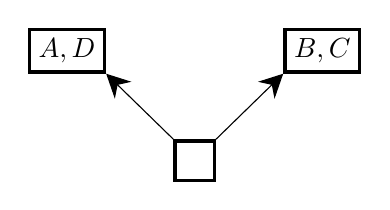
\begin{tikzpicture}[squarednode/.style={rectangle, draw, very thick, minimum size=5mm}]
				\node (center) {};
				\node[squarednode]      (right)   [right=of center] {$B, C$};
				\node[squarednode]      (left)    [left=of center] {$A, D$};
				\node[squarednode]      (lower)       	[below=of center] {};
				\draw[-{Stealth[length=3mm, width=3mm]}] (lower.north west) -- (left.south east);
				\draw[-{Stealth[length=3mm, width=3mm]}] (lower.north east) -- (right.south west);			
			\end{tikzpicture}
		\end{center}
		\captionsetup{justification=centering}
		\caption{ Counter-model $\bigwedge S\to E$.\\(Example 4.1.16.)}
		\label{fi2}
	\end{wrapfigure}

	Essentially, what this tells us is that for every $u$ at which $\psi$ is fulfilled, in particular for each $u$ in the image of $f_\psi$, we may add the assumption that $f_\psi(w) = w$ for all $w\geq u$ without changing the validity of $\psi$.
	With this lemma in hand, showing that $(M_T, I_T)$ is a counter-model to $\varphi^\circ$ is a straightforward check of definitions.

	\begin{corollary}
		If $\mathcal M$ is a counter-model to $\varphi^\circ$ then so is $\mathcal M_T$.
	\end{corollary}

	\addtocounter{theorem}{1}
	\noindent\textbf{Example \thetheorem.} Consider $$\mathcal S = \{(A\to B)\to C, (B\to A)\to D, (A\wedge B)\to \bot, (C\vee D)\to E\}$$

		
	\begin{wrapfigure}[12]{r}{0.5\textwidth}
		\vspace*{-.6cm}
		\begin{center}
			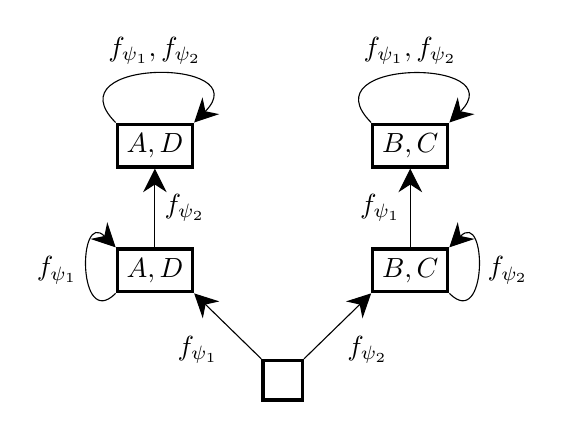
\begin{tikzpicture}[squarednode/.style={rectangle, draw, very thick, minimum size=5mm}]
				\node (center) {};
				\node[squarednode]      (right1)   [right=of center] {$B, C$};
				\node[squarednode]      (right2)   [above=of right1] {$B, C$};
				\node[squarednode]      (left1)    [left=of center] {$A, D$};
				\node[squarednode]      (left2)    [above=of left1] {$A, D$};
				\node[squarednode]      (lower)       	[below=of center] {};
				\draw[-{Stealth[length=3mm, width=3mm]}] (lower.north west) -- (left1.south east) node [midway, below left] {$f_{\psi_1}$};
				\draw[-{Stealth[length=3mm, width=3mm]}] (lower.north east) -- (right1.south west) node [midway, below right] {$f_{\psi_2}$};
				\draw[-{Stealth[length=3mm, width=3mm]}] (left1.north) -- (left2.south) node [midway, right] {$f_{\psi_2}$};
				\draw[-{Stealth[length=3mm, width=3mm]}] (right1.north) -- (right2.south) node [midway, left] {$f_{\psi_1}$};
				\draw[-{Stealth[length=3mm, width=3mm]}] (left1.south west) to [out=225, in=135, loop, looseness=3] node [left] {$f_{\psi_1}$} (left1.north west);		
				\draw[-{Stealth[length=3mm, width=3mm]}] (right1.south east) to [out=315, in=45, loop, looseness=3] node [right] {$f_{\psi_2}$} (right1.north east);
				\draw[-{Stealth[length=3mm, width=3mm]}] (left2.north west) to [out=135, in=45, loop, looseness=3] node [midway, above] {$f_{\psi_1}, f_{\psi_2}$} (left2.north east);
				\draw[-{Stealth[length=3mm, width=3mm]}] (right2.north west) to [out=135, in=45, loop, looseness=3] node [midway, above] {$f_{\psi_1}, f_{\psi_2}$} (right2.north east);		
			\end{tikzpicture}
		\end{center}
		\caption{$\mathcal M_T$}
		\label{fi3}
	\end{wrapfigure}


	and $\varphi = \bigwedge S\to E$ which has the Kripke counter-model depicted in~\ref{fi2}
	where at each node the true propositions are indicated.

		There is a corresponding classical counter-model $\mathcal M = (M, I)$ to $\varphi^\circ$ with $M = \{u, u_l, u_r\}$, $A^{I}(l) = D^I(l) = B^I(r) = C^I(r) = 1$ and $0$ else.
		%
		Denoting $\psi_1 := (A\to B)\to C$ and $\psi_2 := (B\to A)\to D$, this corresponds to a transformed counter-model $\mathcal M_T = (M_T, I_T)$ of $\varphi^\circ$ and interpretation as presented in~\ref{fi3}.\\
	
	\begin{remark}
		It is well known that Kripke frames which are trees are complete with regard to intuitionistic logic. Our contribution is giving an explicit geometry that depends only on the structure of the considered formula.
	\end{remark}
	
	
	So we know that $\varphi^\circ$ is valid if and only if it is valid for structures that have as a domain the sequences without repetition over $\mathcal F_\to$, ordered by the prefix-relation and $$s^I = \epsilon, f_\psi^I(x) = \begin{cases}
		x, &\text{ if $\psi$ occurs in $x$,}\\
		x\psi, &\text{ otherwise.}
	\end{cases}$$
	Now we can replace every $\forall$-quantifier by enumerating all the ground terms, and then replace all distinct ground instances of relations by new propositional variables yielding a propositional formula. This gives us the following theorem.
	
	\begin{theorem}
		Let $\mathcal S$ be a set of formulas of the form
		$$(A\wedge B)\to C, (A\vee B)\to C, A\to (B\wedge C), A\to(B\vee C), (A\to B)\to C$$
		and $\mathcal F_\to\subseteq\mathcal S$ denote the subset of formulas of the form $(A\to B)\to C$ and $\Lambda$ denote the set of sequences without repetition over $\mathcal F_\to$. For each atom $A$ and $k\in\Lambda$ consider a new atom $A^k$. Obtain $\mathcal S^\#$ by including the following formulas:
		\begin{itemize}
			\item $A^k\to A^{k\psi}$ for each atom $A$ occurring in $\mathcal S$, $k\in\Lambda$ and $\psi\in\mathcal F_\to$ not occurring in $k$.
			\item $A^k\to (B^k\circ C^k)$ for each $\circ\in\{\wedge,\vee\}$, $A\to (B\circ C)\in\mathcal S$, $k\in\Lambda$.
			\item $(A^k\circ B^k)\to C^k$ for each $\circ\in\{\wedge,\vee\}$, $A\to (B\circ C)\in\mathcal S$, $k\in\Lambda$.
			\item $(A^{k\psi}\to B^{k\psi})\to C^k$ for $\psi = (A\to B)\to C\in\mathcal S$, $k\in\Lambda$ if $\psi$ does not occurr in $k$.
		\end{itemize}
		Then, $\bigwedge S\to P$ is intuitionistically valid iff $\bigwedge S^\#\to P^\epsilon$ is classically valid, where $\epsilon$ denotes the empty sequence. The size of $\mathcal S^\#$ is in $\mathcal O(|\mathcal S|\cdot2^{|\mathcal F_\to|\cdot\log(|\mathcal F_\to|)})$. Furthermore, there is an effective procedure for translating counter-models between the sentences.
	\end{theorem}

	\begin{example}
		Let us consider the law of excluded middle $\varphi = A\vee\neg A$. Then we get
		$$\mathcal S^-(\varphi) = \{(P_A\vee P_{\neg A})\to P_\varphi, A\to P_A, (A\to \bot)\to P_{\neg A}\},$$
		and we know that $\varphi$ is valid iff $\bigwedge \mathcal S^-(\varphi)\to P_\varphi$ is valid. Applying the above it is intuitionistically valid iff $\bigwedge\mathcal S^\#\to P^\emptyset_\varphi$ is classically valid, where, setting $\psi = (A\to \bot)\to P_{\neg A}$,
		\begin{align*}
			\mathcal S^\# =&\{P_\varphi^\epsilon\to P_\varphi^{\psi}, P_A^\epsilon\to P_A^{\psi},P_{\neg A}^\epsilon\to P_{\neg A}^{\psi},A^\epsilon\to A^{\psi}, (P_A^\epsilon\vee P_{\neg A}^\epsilon)\to P_\varphi^\epsilon, (P_A^{\psi}\vee P_{\neg A}^{\psi})\to P_\varphi^{\psi}\}\cup\\ &\{A^\epsilon\to P_A^\epsilon, P_A^{\psi}\to P_A^{\psi}, (A^{\psi}\to \bot)\to P_{\neg A}^\epsilon, (A^{\psi}\to \bot)\to P_{\neg A}^{\psi}\}.
		\end{align*}
		We now note that $P_\varphi^\epsilon  = P_A^\epsilon = P_{\neg A}^\epsilon = A^\epsilon = 0$, $P_{\varphi}^{\psi} = P_A^{\psi} =  P_{\neg A}^{\psi} = A^{\psi} = 1$ defines a counter-model.
	\end{example}
	
	\section{IPC to QBF}
	
	It is known that a polynomial time translation between QBF and IPC must exist, since both problems are PSPACE complete~\cite{garey1979computers, statman1979intuitionistic}.
	However, giving an explicit translation from IPC to QBF still promises to be useful, allowing to leverage the progress in QBF solving.
	The translation from the last section will serve as starting point for developing the translation in this section.
	We do not define the semantics of QBF and refer the reader to standard sources e.g.~\cite{series/faia/2009-185}.
	
	Fix some set $\mathcal S$ of formulas of the form $$A\to (B\wedge C), (A\wedge B)\to C, A\to (B\vee C), (A\vee B)\to C, (A\to B)\to C$$and$$\varphi = \bigwedge \mathcal S\to P,$$
	and denote with $\mathcal F_\to$ the set of formulas of the form $(A\to B)\to C$. We will now formulate a QBF that expresses that $\varphi$ has an intuitionistic counter-model. The idea how to get a polynomially-sized formula is: Instead of expressing validity at every node of $\mathcal M_T$ --- which was done in the CPC translation --- we express that on each path in $\mathcal M_T$ the nodes satisfy all conditions for $\mathcal M_T$ being a counter-model. The universally quantified variables $F_\psi$ in the next definition handle the branching, i.e. express which path is considered.
	
	\begin{definition}
		For every propositional variable $X$ occurring in $\mathcal S$ and non-negative integer $n$ consider a new atom $X^n$ and for every formula $\psi\in\mathcal F_\to$ consider a new atom $F_\psi^n$. Let $\vec X^n$ range over all propositional variables $X^n$ and $\vec F^n$ range over all $F_\psi^n$. Define
		\begin{itemize}
			\item {\normalfont Valid}$(n)$, which encodes that $\vec F^n_\psi$ represents a valid next element of a sequence without repetition, i.e. if we interpret the $\vec F^i$ as bit-vectors, then $\vec F^n$ has exactly one bit set to $1$, indicating the formula at the $n$-th position of the sequence, and it is at a position that is $0$ in $\sum\{\vec F^i\:|\:i < n\}$.
			\item {\normalfont Persistent}$(n)$, which encodes that the persistency condition holds.
			\item {\normalfont Sat}$_{\mathcal S}(n)$, encoding that the formulas in $\mathcal S\setminus\mathcal F_\to$ hold at the $n$-th world of the path.
			\item {\normalfont Sat}$_{\mathcal F_\to}(n)$, encoding that the formula in $\mathcal F_\to$ that is represented by $\vec F^{n-1}$ holds.
		\end{itemize}
		Have $k = |\mathcal F_\to|$ and define$$\varphi^Q_{i} = \exists \vec X^i\forall \vec F^i\left(\text{\normalfont Persistent}(i)\wedge \text{\normalfont Sat}_{\mathcal S}(i)\wedge \text{\normalfont Sat}_{\mathcal F_\to}(i)\wedge\left(\text{\normalfont Valid}(i)\to \varphi^Q_{i+1}\right)\right)$$
		for $0 < i < k$, as well as the special cases
		$$\varphi^Q_{k} = \exists \vec X^k\left(\text{\normalfont Persistent}(k)\wedge \text{\normalfont Sat}_{\mathcal S}(k)\wedge \text{\normalfont Sat}_{\mathcal F_\to}(k)\right)$$
		for leafs, and $$\varphi^Q = \varphi_0^Q = \exists \vec X^0\forall \vec F^0\left(\neg P^0\wedge \text{\normalfont Sat}_{\mathcal S}(0)\wedge(\text{\normalfont Valid}(0)\to \varphi_1^Q)\right)$$for the root.
		Example encodings of the above formulas are:
		\begin{align*}
			\text{\normalfont Valid}(n) = &\left(\bigvee \{\mathcal F^n_\psi\:|\:\psi\in\mathcal F_\to\}\right)\wedge\left(\bigwedge \{\neg(F^n_{\psi_1}\wedge F^n_{\psi_1})\:|\:\psi_1\neq\psi_2\in\mathcal F_\to\}\right)\wedge\\&\left(\bigwedge\left\{\bigwedge\{F^i_\psi\to\neg F^n_\psi\:|\:i < n\}\:|\:\psi\in\mathcal F_\to\right\}\right)\\
			\text{\normalfont Persistent}(n) = & \bigwedge\{X^{n-1}\to X^n\:|\: X \text{ prop. variable with }X^{n-1}\in\vec X^{n-1}, X^n \in\vec X^{n}\}\\
			\text{\normalfont Sat}_{\mathcal S}(n) = &\bigwedge\left\{(A^n\circ B^n)\to C^n\:|\:(A\circ B)\to C\in \mathcal S\setminus\mathcal F_\to\right\}\wedge\\
			&\bigwedge\left\{A^n\to (B^n\circ C^n)\:|\:A\to (B\circ C)\in \mathcal S\setminus\mathcal F_\to\right\}\\
			\text{\normalfont Sat}_{\mathcal F_\to}(n) = & \bigwedge\{F^{n-1}_\psi\to (A^n\to B^n)\to C^{n-1}\:|\:\psi = (A\to B)\to C\in\mathcal F_\to\}
		\end{align*}
	\end{definition}
	
	\begin{example}
		With the previous encoding for the double negation elimination $$\varphi = ((A\to \bot)\to \bot)\to A$$ we have
		$$\hspace*{-.3cm}
		\varphi^Q = \exists A^0\forall F^0\left(\neg A^0\wedge\left(F^0\to \exists A^1\left((A^0\to A^1)\wedge(F_0\to (A^1\to \bot)\to \bot)\right)\right)\right),
		$$
		which is a satisfiable QBF since $A^0 = 0, A^1 = 1$ satisfies it for any $F^0$.
	\end{example}
	
	
	\begin{lemma}
		$\varphi$ is not intuitionistically valid iff $\varphi^Q$ is a satisfiable QBF.
	\end{lemma}
	
	\begin{proof}
		Suppose $\varphi$ is not intuitionistically valid.
		Then, $\bigwedge\mathcal S\to P$ has an intuitionistic counter-model. Then, by the previous section there exists a classical counter-model $\mathcal M$ for $\bigwedge\mathcal S^\#\to P^\epsilon$.
		We now define a QBF model iteratively.
		For each atom $A$ interpret $A^0$ such as $\mathcal M$ interprets $A^\epsilon$. Suppose we are given interpretations of all atoms $A^i$ for $i < n$ and a sequence with no repetitions $\psi_1\dots\psi_{n-1}$ over $\mathcal F_\to$ such that $\psi_i$ is exactly the $\psi\in\mathcal F_\to$ for which $F_{\psi}^i$ is true and $A^i$ is interpreted as $A^{\psi_1\dots\psi_i}$  in $\mathcal M$.
		Let the $F^{n}_\psi$ be arbitrarily interpreted (since they are $\forall$-quantified). If not exactly one of the $F^{n}_\psi$ is interpreted as true, then valid$(n)$ fails and the remaining propositions can be chosen arbitrarily. If $F^i_{\psi_n} = 1$ for some $i < n$, then valid$(n)$ also fails and the remaining propositions can be chosen arbitrarily.
		So we may assume that $\psi_1\dots\psi_n$ is a sequence with no repetitions.
		Interpret the atoms $A^n$ as $\mathcal M$ interprets $A^{\psi_1\dots\psi_n}$.
		Continue this construction until $n  = |\mathcal F_\to|$. Then from $\mathcal M$ being a counter-example to $\mathcal S^\#\to P$ it directly follows that this interpretation satisfies $\varphi^Q$.
		
		On the other hand, suppose $\varphi^Q$ is satisfiable. We construct a counter-example to $\varphi^\#$.
		Again, we proceed iteratively. Interpret $A^\epsilon$ such as $A^0$ is interpreted in some satisfying interpretation of $\varphi^Q$. Suppose we are given a sequence $\psi_1\dots \psi_{n-1}$ such that for $i<n$ having $A^i = A^{\psi_0\dots\psi_{n-1}}$ is part of a satisfying interpretation of $\varphi^Q$, in which $F^i_\psi$ is chosen true iff $\psi = \psi_i$. Let $\psi_n\in\mathcal F_\to$. Consider some interpretation of the $A^n$ that are part of a satisfying assignment where $F^n_\psi$ is true iff $\psi = \psi_n$ and all variables quantified above are chosen as before. Have $A^{\psi_0\dots\psi_n} = A^n$ for each propositional variable $A$. From the definitions it directly follows that construction yields a counter-model for $\varphi^\#$.
	\end{proof}
	
	A simple counting argument shows that for each $n < |\mathcal F_\to|$ we have $|\text{Valid}(n)|\in \mathcal O(|\mathcal F_\to|^2)$, $|\text{Persistent}(n)|, |\text{Sat}_{\mathcal S}(n)|\in \mathcal O(|\varphi|)$ and $|\text{Sat}_{\mathcal F_\to}(n)|\in \mathcal O(|\mathcal F_\to|)$ so overall we get:
	\begin{lemma}
		The size of $\varphi^Q$ is in $\mathcal O(|\varphi|\cdot|\mathcal F_\to| + |\mathcal F_\to|^3)$.
	\end{lemma}
	
	Note that the last set of universally quantified variables can be avoided because there is only one assignment that has the chance to falsify $\varphi^Q$, namely the assignment that assigns $1$ to the single $F_\psi^n$ such that $F_\psi^i = 0$ for all $i < n$. Hence, in our final formula we can replace every $F_\psi^n$ with $\bigwedge\{\neg F_\psi^i\:|\:i < n\}$ and remove that quantification over $F_\psi^n$. With that we get the following:
	
	\begin{corollary}
		Let $N$-\verb+IntInvalid+ be the problem of deciding if a formula $\bigwedge \mathcal S\to P$ as above with $|\mathcal F_\to|\leq N$ is not intuitionistically valid. Then $N$-\verb+IntInvalid+ is in $\Sigma_{2N-1}^P$. The dual problem $N$-\verb+IntValid+ is in $\Pi_{2N-1}^P$.
	\end{corollary}
	
	\section{CQC to IQC}\label{section:CQCIQC}
	
	We now give an analogous transformation for first order logic. Our trick of lifting the sentence to first-order logic to encode the Kripke semantics no longer works in such a straightforward manner, since we already are in first-order logic. However, we do it nonetheless! The domain of our classical model will feature on the one hand elements representing worlds in a Kripke frame and on the other hand the domain-elements from the Kripke model. We reconcile these notions by introducing a special binary predicate $E$, first considered in~\cite{baaz2006skolemization} and expanded onto in~\cite{iemhoff2010eskolemization}, where $E(x, u)$ encodes that $x$ is an element of the domain of the world $u$. We fix some signature $\Sigma$ for this section. To encode that some $n$-ary relation $A$ holds at a world $u$ we replace each $n$-ary relation symbol $A$ with a $n+1$-ary relation symbol $A^\#$, interpreting $A^\#(\vec x, u)$ as ``$A(\vec x)$ holds at $u$''. Furthermore we write $\vec E(\vec x, u)$ for $\bigwedge\{E(x_i, u)\:|\:x_i\in \vec x\}$.
	
	First of all recall, that due to Lemma~\ref{equivalid} it is sufficient to consider sentences of the form $\bigwedge\mathcal S\to P$ where all formulas in $\mathcal S$ are of one of the forms
	\[\begin{matrix}
		\forall \vec z(A(\vec a)\to (B(\vec b)\wedge C(\vec c)))\indent \forall \vec z((A(\vec a)\wedge B(\vec b))\to C(\vec c))\indent \forall \vec z(A(\vec a)\to (B(\vec b)\vee C(\vec c)))\\
		\forall \vec z((A(\vec a)\vee B(\vec b))\to C(\vec c))\indent \forall \vec z((A(\vec a)\to B(\vec b))\to C(\vec c))\indent\forall \vec z(\forall xA(\vec a)\to B(\vec b))\\ \forall \vec z(A(\vec a)\to\forall xB(\vec b))\indent \forall \vec z(\exists xA(\vec a)\to B(\vec b))\indent\forall \vec z(A(\vec a)\to\exists xB(b)).
	\end{matrix}\]
	The complete result that we will show is as follows:
	\begin{theorem}\label{fullFOtranslation}
		Let $\mathcal S$ be as above and $\mathcal F_\to\subseteq\mathcal S$ contain the formulas of the form $\forall \vec t((A(\vec z_A)\to B(\vec z_B))\to C(\vec z_C))$ and $\mathcal F_\forall\subseteq\mathcal S$ the formulas of the form $\forall \vec z(\forall xA(\vec z_A)\to B(\vec z_B))$. Let $\mathcal F = \mathcal F_\to\cup\mathcal F_\forall$. For every $n$-ary atomic relation $R$ define a new $n+1$-ary relation $R^\#$. For every $\psi\in\mathcal F$ define a new function symbol $f_\psi$. Consider a new binary relation symbol $E$ and define $\vec E(\vec x, u) := \bigwedge\{E(x, u)\:|\:x\in\vec x\}$. Obtain $\mathcal S^\#$ by including formulas as follows:
		\begin{itemize}
			\item $\forall \vec z\forall u(\vec E(\vec z, u)\to (A^\#(\vec a, u)\to (B^\#(\vec b, u)\circ C^\#(\vec c, u))))$\\for each $\circ\in\{\wedge, \vee\}, \psi = \forall \vec z(A(\vec a)\to (B(\vec b)\circ C(\vec c)))\in\mathcal S$
			\item $\forall \vec z\forall u(\vec E(\vec z, u)\to (A^\#(\vec a, u)\circ B^\#(\vec b, u))\to C^\#(\vec c, u))$\\for each $\circ\in\{\wedge, \vee\}, \psi = \forall \vec z((A(\vec a)\circ B(\vec b))\to C(\vec c))\in\mathcal S$
			\item $\forall \vec z\forall u(\vec E(\vec z, u)\to(A^\#(\vec a, f_\psi(\vec z, u))\to B^\#(\vec b, f_\psi(\vec z, u)))\to C^\#(\vec c, u))$\\for each $\psi = \forall \vec z((A(\vec a)\to B(\vec b))\to C(\vec c))\in\mathcal S$
			\item  $\forall \vec z\forall u(\vec E(\vec z, u)\to \forall x(E(x, f_\psi(\vec z, u))\to A^\#(\vec a, f_\psi(\vec z, u)))\to B^\#(\vec b, u))$\\for each $\psi = \forall \vec z(\forall xA(\vec a)\to B(\vec t_B))\in\mathcal S$.
			\item $\forall \vec z\forall u(\vec E(\vec z, u)\to A^\#(\vec a, u)\to \forall x(E(x, u)\to B^\#(\vec b, u)))$\\for each $\forall \vec t(A(\vec a)\to \forall xB(\vec b))\in\mathcal S$.
			\item $\forall \vec z\forall u(\vec E(\vec z, u)\to \exists x(E(x, u)\wedge A^\#(\vec z, u))\to B^\#(\vec b))$\\for each $\forall \vec z(\exists xA(\vec a)\to B(\vec b))\in\mathcal S$
			\item $\forall \vec z\forall u(\vec E(\vec z, u)\to A^\#(\vec b)\to \exists x(E(x, u)\wedge B^\#(\vec b, u)))$\\for each $\forall \vec z(A(\vec a)\to \exists xB(\vec b))\in\mathcal S$
		\end{itemize}
		Then $\bigwedge S\to P$ is intuitionistically iff $\exists xE(x, s)\to K\to \bigwedge\mathcal S^\#\to P^\#(s)$ is classically valid, where $s$ is a new constant symbol, $\Sigma$ is the original signature and
		\begin{align*}
			K := &\:\bigwedge\{\forall\vec z\forall x\forall u((E(x, u)\to E(x, f_\psi(\vec z, u)))\:|\:\psi\in\mathcal F\}\wedge\\
			&\:\forall u\left(\exists xE(x, u)\to \bigwedge\{\forall\vec z(\vec E(\vec z, u)\to E(f(\vec z), u))\:|\:\text{$f$ is a function symbol in $\Sigma$}\}\right)\wedge\\
			&\:\bigwedge\{\forall\vec z_1\forall \vec z_2\forall u(A^\#(\vec z_1, u)\to A^\#(\vec z_1, f_\psi(\vec z_2, u)))\:|\:\text{$\psi\in\mathcal F$, $A$ is a relation symbol in $\Sigma$}\}.
		\end{align*}
		The size of the obtained formula is linear in the input. However $|\mathcal F| + 1$ new function symbols and the new binary predicate $E$ were introduced and each $n$-ary relation symbol has been extended to a $n+1$-ary relation symbol.
	\end{theorem}
	
		
	\begin{example}
		Consider the classical tautology $\varphi := \neg\forall x\neg A(x)\to \exists x A(x)$. Setting $\psi := \forall x\neg A(x)$ we have
		\begin{align*}
			S^\#(\varphi) = &\{\forall u((P_{\neg\psi}^\#(f_\varphi(u))\to P_{\exists xA(x)}^\#(f_\varphi(u)))\to P_\varphi^\#(u))\}\cup\\
			 & \{\forall u(\exists x(E(x, u)\wedge A^\#(x, u))\to P_{\exists xA(x)}^\#(u)), \forall u((P_{\neg\psi}^\#(u)\wedge P^\#_\psi(u))\to \bot)\}\cup\\
			 & \{\forall u(\forall x(E^\#(x,f_\psi(u))\to P^\#_{\neg A(x)}(x, f_\psi(u)))\to P^\#_\psi(u))\}\cup\\&\{ \forall x\forall u(E(x, u)\to (A^\#(x, f_{\neg A(x)(u)})\to \bot)\to P^\#_{\neg A(x)}(x, u))\}
		\end{align*}
		And as one might expect we can indeed define a counter-model for $$\exists xE(x, s)\to K\to\bigwedge S^\#\to P^\#(s),$$
		namely take as a domain $M = \{m, v, w\}$ where $u, w$ represent worlds, and $m$ representing a single domain element. Have $f_\varphi^I(x) = f_\psi^I(x) = f_{\neg A(x)}^I(x) = w$ for all $x\in M$, $E^I(x, y)$ if and only if $x = m$ and $y\in\{u, v\}$ and finally $A^\#(x, y)$ iff $x = m$ and $y = w$.
	\end{example}
	
	It is not possible to completely eliminate worlds from the domain as in the propositional case, since counter-models can possibly be infinite (as we will see in more detail later).

	
	\subsection{Encoding Kripke Semantics}
	
	As in the propositional case we must encode the Kripke Semantics, this time not only the relation $\preceq$, but also $E$ has to be axiomatized. For that we use the following predicates:
	\begin{itemize}
		\item PartialOrder($\preceq$), encoding that $\preceq$ is a partial order.
		\item DomainSubset$(u, w)$, encoding that the domain at $u$ is a subset of that at $w$.
		\item World($u$), encoding that $u$ represents a world.
		\item DomainClosed($u$), which encodes that at $u$ the domain is closed under functions, e.g. contains all interpretations of constants.
		\item Persistent$(u, w)$, which encodes that persistency is satisfied between $u$ and $w$, i.e. for all predicates $A$ and domain elements $x$ with $A(x)$, at $u$ we have $A(x)$ at $w$.
	\end{itemize}
	Then, analogously to the propositional case, we define:
	\begin{align*}
		K(\varphi) = \:& \text{PartialOrder}(\preceq) \wedge \forall u \forall w (u\preceq w\to \text{DomainSubset}(u, w)) \wedge\\
		& \forall u(\text{World(u)}\to \text{DomainClosed}(u))\wedge \forall u\forall w (u\preceq w\to \text{Persistent}(u, w)).
	\end{align*}
	Example encodings of these formulas are as follows:
	\begin{align*}
		\text{PartialOrder}(\preceq) = &\:\forall u(u\preceq u)\wedge\forall u\forall w(u\preceq w\to w\preceq u\to u = w)\wedge\\&\:\forall u\forall v\forall w(u\preceq v\to v\preceq w\to u\preceq w)\\
		\text{DomainSubset}(u, w) = &\:\forall z(E(z, u)\to E(z, w))\\
		\text{World}(u) = &\:\exists xE(x, u)\\
		\text{DomainClosed}(u) = &\:\bigwedge\{\forall\vec z(\vec E(\vec z, u)\to E(f(\vec z), u))\:|\:\text{$f\in\Sigma$ is a function symbol}\}\\
		\text{Pesistent}(u, w) = &\:\bigwedge\{\forall\vec z(\vec A^\#(\vec z, u)\to A^\#(\vec z, w))\:|\:\text{$A\in\Sigma$ is a relation symbol}\}
	\end{align*}
	
	Using $E$, we then obtain $\mathcal S'$ analogously to the predicate case by including formulas:
	
	\begin{itemize}
		\item $\forall \vec z\forall u(s\preceq u\to \vec E(\vec z, u)\to (A^\#(\vec a, u)\to (B^\#(\vec b, u)\circ C^\#(\vec c, u))))$\\for each $\circ\in\{\wedge, \vee\}, \psi = \forall \vec z(A(\vec a)\to (B(\vec b)\circ C(\vec c)))\in\mathcal S$
		\item $\forall \vec z\forall u(s\preceq u\to\vec E(\vec z, u)\to (A^\#(\vec a, u)\circ B^\#(\vec b, u))\to C^\#(\vec c, u))$\\for each $\circ\in\{\wedge, \vee\}, \psi = \forall \vec z((A(\vec a)\circ B(\vec b))\to C(\vec c))\in\mathcal S$
		\item $\forall \vec z\forall u(s\preceq u\to\vec E(\vec z, u)\to\forall w(u\preceq w\to A^\#(\vec a, w)\to B^\#(\vec b, w))\to C^\#(\vec c, u))$\\ for each $\psi = \forall \vec z((A(\vec a)\to B(\vec b))\to C(\vec c))\in\mathcal S$
		\item  $\forall \vec z\forall u(s\preceq u\to\vec E(\vec z, u)\to \forall w(u\preceq w\to \forall x(E(x, w)\to A^\#(\vec a, w)))\to B^\#(\vec b, u))$\\for each $\forall \vec z(\forall xA(\vec a)\to B(\vec t_B))\in\mathcal S$.
		\item $\forall \vec z\forall u(s\preceq u\to\vec E(\vec z, u)\to A^\#(\vec a, u)\to \forall x(E(x, u)\to B^\#(\vec b, u)))$\\for each $\forall \vec t(A(\vec a)\to \forall xB(\vec b))\in\mathcal S$.
		\item $\forall \vec z\forall u(s\preceq u\to\vec E(\vec z, u)\to \exists x(E(x, u)\wedge A^\#(\vec z, u))\to B^\#(\vec b, u))$\\for each $\forall \vec z(\exists xA(\vec a)\to B(\vec b))\in\mathcal S$
		\item $\forall \vec z\forall u(s\preceq u\to\vec E(\vec z, u)\to A^\#(\vec b, u)\to \exists x(E(x, u)\wedge B^\#(\vec b, u)))$\\for each $\forall \vec z(A(\vec a)\to \exists xB(\vec b))\in\mathcal S$
	\end{itemize}
	
	Then $\varphi = \bigwedge\mathcal S\to P$ is intuitionistically valid if and only if
	$$\varphi' = \text{World}(s)\to K(\varphi)\to \bigwedge S'\to P^\#(s)$$
	is classically valid, where $s$ is a new constant symbol. This was obvious in the propositional case but here it is more nuanced.
	
	\begin{proof}
		We proceed by translation of counter-examples. Suppose first we have a counter-example $\mathcal M = (M, I)$ to $\varphi'$. As a Kripke frame $(W, \leq)$ take all $ W = \{m\in M\:|\:\text{ World}^I(m)\}$ let $\leq$ be $\preceq^I$ restricted to $W$. Then let $M_u = \{m\in M\:|\: E(m, u)\}$ and let $f^{I_u}$ be $f^I$ restricted to $M_u$ and $A^{I_u}(\vec x): \Leftrightarrow A^\#(\vec x, u)$. It is then a straightforward check of definitions that this defines a Kripke counter-model to $\varphi$.
		
		The other direction is a bit more involved. Suppose we have a Kripke counter-model to $\varphi$ with frame $(W, \preceq)$ and family of $\Sigma$-structures $(M_w, I_w)_{w\in W}$. In particular, since it is a counter-model there exists $w_0\in W$ with $w_0\not\models\varphi$. Let $W_0 = \{w\in W\:|\: w\geq w_0\}$ and define an equivalence relation $\sim$ on $\{(x, u)\:|\:u\in W_0, x\in M_u\}$ via $(x, u)\sim (y, w)$ iff $x = y$ and there exists $v\in W_0$ comparable with both $u, w$ such that $x\in v$ and denote the equivalence class of $(x, u)$ with $[x, u]$. Let $M = W_0\cup \{[x, u]\:|\:u\in W_0, x\in M_u\}$.
		Now have
		\begin{itemize}
			\item $s^I = w_0$.
			\item $E^I(m, w)$ iff $w\in W_0$ and $m \sim [x, w]$ for some $x\in M_w$.
			\item $f^I(m_1\dots m_n) =\begin{cases}
				f^{I_u}(x_1\dots x_n), &\text{if there are $ u\in W_0, x_i\in M_u$ with $m_i\sim [x_i, u]$ for all $i$,}\\
				w_0, & \text{otherwise.}
			\end{cases}$
			\item ${A^\#}^I(m_1\dots m_n, u) \Leftrightarrow\begin{cases}
				A^{I_u}(x_1\dots x_n), &\text{if $u\in W_0$ and $\exists x_i\in M_u$ w. $m_i\sim [x_i, u]$ for all $i$,}\\
				\top, & \text{otherwise.}
			\end{cases}$
		\end{itemize}
		One easily verifies that these are well-defined. Let us now briefly check that this indeed defines a counter-model. First of all ${P^\#}^I(s^I)$ is false since $P^{I_{w_0}}$ is. Clearly World$(w_0)$ holds and $K(\varphi)$ is also easily verified. All that remains to show is $M, I\models\bigwedge\mathcal S'$. Consider e.g. the case where $\psi\in\mathcal S$ is of the form
		$$ \forall \vec z((A(\vec a)\to B(\vec b))\to C(\vec c))$$
		We have to show that
		$$M, I\models \forall \vec z\forall u(\vec E(t, u)\to \forall w(u\preceq w\to A^\#(\vec a, w)\to B^\#(\vec b, w))\to C^\#(\vec c, u))$$
		holds. Suppose towards contradiction that it does not, i.e. there are $u, \vec z\in M$ such that for all $w\in M$
		$$\vec E^I(\vec z, u)\to (u\preceq w\to {A^\#}^I(\vec a, w)\to {B^\#}^I(\vec b, w))\to {C^\#}^I(\vec c, u)$$ is false. For that ${C^\#}^I(\vec c, u)$ must be false and in particular $u\in W_0$. Futhermore $\vec E^I(\vec z, u)$ must be true and we can write $\vec z = [z_1, u]\dots[z_n, u]$ for some $z_i\in W_u$. Note that the above is false in particular for $w\in M_0$ with $u\preceq w$. But this would imply
		$$((A^{I_u}(\vec a)\to B^{I_u}(\vec b))\to C^{I_u}(\vec c))[\vec z/z_1\dots z_n]$$in our original Kripke counter-model. The other cases are analogous.
	\end{proof}
	
	\subsection{Reducing the encoding}
	
	As in the predicate case, we now show the existence of a canonical counter-model (in case such a counter-model exists). Denote the set of formulas $\psi\in\mathcal S$ of the form $\forall\vec z((A(\vec a)\to B(\vec b))\to C(\vec c))$ with $\mathcal F_\to$ and of the form $\forall \vec z(\forall xA(\vec a)\to B(\vec b))$ with $\mathcal F_\forall$. Let $\mathcal F = \mathcal F_\to\cup\mathcal F_\forall$. For each  $\psi\in\mathcal F$ consider a new function symbol $f_\psi$. As before we may assume that $s$ is a least element and we can avoid the quantification over $w$ by considering the formulas
	\begin{itemize}
		\item $\forall \vec z\forall u(\vec E(\vec z, u)\to (A^\#(\vec a, f_\psi(\vec z, u))\to B^\#(\vec b, f_\psi(\vec z, u)))\to C^\#(\vec c, u))$\\instead of $\forall \vec z\forall u(s\preceq u\to\vec E(\vec z, u)\to \forall w(u\preceq w\to A^\#(\vec a, w)\to B^\#(\vec b, w))\to C^\#(\vec c, u))$,
		\item $\forall \vec z\forall u(\vec E(\vec z, u)\to (\forall x(E(x, f_\psi(\vec z, u))\to A^\#(\vec a, f_\psi(\vec z, u))))\to B^\#(\vec b, u))$\\instead of $\forall \vec z\forall u(s\preceq u\to\vec E(\vec z, u)\to \forall w(u\preceq w\to \forall x(E(x, w)\to A^\#(\vec a, w)))\to B^\#(\vec b, u))$,
	\end{itemize}
	and by removing removing the $s\preceq u$ for the remaining formulas in $\mathcal S'$.
	We denote the resulting set of formulas by $\mathcal S^\#$.
	Then, the previous formulas are equivalid to
	$$\varphi^\circ= \forall u(s\preceq u)\to \bigwedge\{\forall \vec t\forall u(u\preceq f(\vec z, u))\:|\:\psi\in\mathcal F\}\to K(\varphi)\to\bigwedge\mathcal S^\#\to P^\#(s).$$
	As in the previous section we can define a tree counter-model for this.
	
	\begin{definition}
		Suppose we are given a counter-model $\mathcal M = (M, I)$ for $\varphi^\circ$. Define $\mathcal M_T = (M_T, I_T)$ as follows:
		\begin{itemize}
			\item $M_T$ are the sequences on $\{(\vec z, \psi)\:|\:\psi\in \mathcal F, \vec z\in M^n\}$.
			\item We interpret $\preceq$ as the prefix-order.
			\item We set $$f_\psi^{I_T}(\vec z, (\vec z_1, \psi_1)\dots (\vec z_n, \psi_n)) = (\vec z_1, \psi_1)\dots (\vec z_n, \psi_n)(\vec z, \psi).$$
			\item For relation symbols $R^\#$, we set $${R^\#}^{I_T}(\vec z, (\vec z_1, \psi_1)\dots (\vec z_n, \psi_n)) = {R^\#}^I(\vec z, f_{\psi_n}(\vec z_n, \dots(f_{\psi_1}(\vec z_1, s^I))\dots)).$$
		\end{itemize}
	\end{definition}
	
	\begin{lemma}
		If $\mathcal M$ is a counter-model to $\varphi^\circ$ then so is $\mathcal M_T$.
	\end{lemma}
	
	Even if we don't have the finiteness property of the propositional case, we have still managed to reduce the complexity of possible counter-models because we know that considering worlds of the form $$f_{\psi_1}(\vec z_1, f_{\psi_2}(\vec z_2, \dots f_{\psi_n}(\vec z_n, s)\dots))$$ is sufficient.
	In particular, this allows us to completely eliminate $\preceq$ from the formula, that is we remove the PartialOrder$(\preceq)$
	from $K(\varphi)$ and adjust DomainSubset$(u, w)$ and Persistent$(u, w)$, e.g. remove quantification over $w$ and the precondition $u\preceq w$ from $K(\varphi)$ and replace DomainSubset$(u, w)$ with
	$$\bigwedge\{\forall \vec z\forall u\forall x(E(x, u)\to E(x, f_\psi(\vec z, u)))\:|\:\psi\in\mathcal F_\to\}$$ and Persistent$(u, w)$ with $$\bigwedge\{\forall\vec z_1\forall\vec z_2\forall u(A(\vec z_1, u)\to A(\vec z_1, f_\psi(\vec z_2, u)))\:|\:\psi\in\mathcal F_\to, \text{$A\in\Sigma$ is a relation symbol}\}.$$ We set
	
	$$\varphi^{\#} = K\to \bigwedge S^\#\to P^\#.$$
	Then, we obtain the following result:
	\begin{theorem}
		\label{thm:fo-reduction}
		$\varphi$ is intuitionistically valid iff $\varphi^\#$ is classically valid.
	\end{theorem}
	The complete translation is summarised in Theorem~\ref{fullFOtranslation} (stated earlier). Let us understand why a further reduction as in the propositional case is impossible. In this case this is not such an issue, because as we started in predicate logic it is not so troublesome that we introduce some additional predicates, however it is still interesting to understand why it is required.
	
	
	\begin{definition}
		\label{def:fo-fulfilled}
		Suppose we are given a counter-model $\mathcal M = (M, I)$ for $\varphi^\circ$. For $\psi = \forall\vec z\psi'\in\mathcal F_\to$ we say it is \emph{fulfilled} at $u\in M$ with $\vec m\in M^n$ iff $(A_\psi^I(\vec a, u)\to B_\psi^I(\vec b, u))[\vec m/\vec z]$ is false or $C_\psi^I(\vec c, u)[\vec m/\vec z]$ is true.
		For $\psi = \forall\vec z\psi'\in\mathcal F_\forall$ we say it is \emph{fulfilled} at $u\in M$ with $\vec m\in M^n$ iff there is $m\in M$ with $E^{I}(m, u)$ such that $A^{I[m/x]}_\psi(\vec a)[\vec m/\vec z]$ is false or $B_\psi^I(\vec b)[\vec m/\vec z]$ is true.
	\end{definition}
	
	We get an analogous result to Lemma~\ref{thm:prop-countermodel-reduction}:
	
	\begin{lemma}
		\label{thm:fo-countermodel-reduction}
		Let $\mathcal M = (M, I)$ be a counter-model to $\mathcal \varphi^\circ$.
		\begin{enumerate}
			\item $\psi$ is fulfilled at $f_\psi^I(\vec a, u)$ with $\vec a$ for all $u\in M, \psi\in\mathcal F$, $\vec a\in M^n$.
			\item If $\psi\in\mathcal F_\to$ is fulfilled at $u\in M$ with $\vec a$ then $\psi$ is fulfilled at all $w\geq u$ with $\vec a$.
		\end{enumerate}	
	\end{lemma}


	However part 2 of Lemma~\ref{thm:fo-countermodel-reduction} fails for $\psi\in\mathcal F_\forall$, because even if for all $x$ with $E(x, v$), we have $A(x, v)$, there could be some term $y$ with $\neg E(y, v)$ and $w$ with $v\preceq w$ such that $E(y, w)$ and $\neg A(y, w)$. This is why we must consider sequences that have repetitions:
	\pagebreak
	\begin{wrapfigure}[16]{r}{0.4\textwidth}
		\begin{center}
			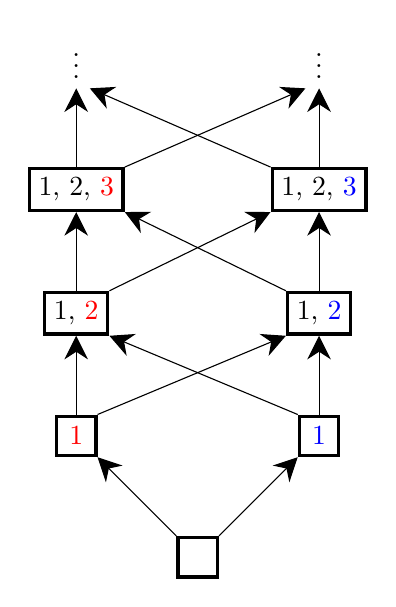
\begin{tikzpicture}[squarednode/.style={rectangle, draw, very thick, minimum size=5mm}]
				\node[squarednode]      (0)   [] {$ $};
				\node[squarednode]      (1r)   [above right=of 0] {{\color{blue}$1$}};
				\node[squarednode]      (1l)   [above left=of 0] {{\color{red}$1$}};
				\node[squarednode]      (2r)   [above=of 1r] {{1, \color{blue}$2$}};
				\node[squarednode]      (2l)   [above=of 1l] {{1, \color{red}$2$}};
				\node[squarednode]      (3r)   [above=of 2r] {{1, 2, \color{blue}$3$}};
				\node[squarednode]      (3l)   [above=of 2l] {{1, 2, \color{red}$3$}};
				\node      (4r)   [above=of 3r] {{$\vdots$}};
				\node      (4l)   [above=of 3l] {{$\vdots$}};
				\draw[-{Stealth[length=3mm, width=3mm]}, color=black] (0.north east) -- (1r.south west);
				\draw[-{Stealth[length=3mm, width=3mm]}, color=black] (0.north west) -- (1l.south east);
				\draw[-{Stealth[length=3mm, width=3mm]}, color=black] (1r.north) -- (2r.south);
				\draw[-{Stealth[length=3mm, width=3mm]}, color=black] (1l.north) -- (2l.south);
				\draw[-{Stealth[length=3mm, width=3mm]}, color=black] (1l.north east) -- (2r.south west);
				\draw[-{Stealth[length=3mm, width=3mm]}, color=black] (1r.north west) -- (2l.south east);
				\draw[-{Stealth[length=3mm, width=3mm]}, color=black] (2r.north) -- (3r.south);
				\draw[-{Stealth[length=3mm, width=3mm]}, color=black] (2l.north) -- (3l.south);
				\draw[-{Stealth[length=3mm, width=3mm]}, color=black] (2l.north east) -- (3r.south west);
				\draw[-{Stealth[length=3mm, width=3mm]}, color=black] (2r.north west) -- (3l.south east);
				\draw[-{Stealth[length=3mm, width=3mm]}, color=black] (3r.north) -- (4r.south);
				\draw[-{Stealth[length=3mm, width=3mm]}, color=black] (3l.north) -- (4l.south);
				\draw[-{Stealth[length=3mm, width=3mm]}, color=black] (3l.north east) -- (4r.south west);
				\draw[-{Stealth[length=3mm, width=3mm]}, color=black] (3r.north west) -- (4l.south east);
			\end{tikzpicture}
		\end{center}
		\caption{Counter-model to $\varphi$.}
		\label{fig1}
	\end{wrapfigure}	
	\
	\begin{example}
		Consider $\varphi = \neg(\neg \forall xA(x)\vee\neg \forall xB(x))$. There is a counter-model as shown in Figure~\ref{fig1},
		where we indicate at each world the elements that exist at it. For black numbers $n$, both $A(n)$ and $B(n)$ hold at that world, for red ones only $A(n)$, for blue ones only $B(n)$. The arrows indicate the order. $\neg\forall xA(x)$ is not fulfilled at worlds in the left column and $\neg\forall xB(x)$ is not fulfilled at worlds in the right column. In particular applying $f_{\neg \forall xA(x)}$ we must always reach the right column and applying $f_{\neg \forall xB(x)}$ we must always reach the left column. Therefore applying $f_{\neg \forall xA(x)}\circ f_{\neg \forall xB(x)}$ we cannot remain stationary.
	\end{example}
	
	Let us add that Lemma~\ref{thm:fo-countermodel-reduction} still equips us with additional information that can be used to guide proof search: We could add additional axioms that restrict the interpretation of functions. That is, we may assume that $f_\psi(w) = w$, if $\exists u(w = f_\psi(u))$ for all $\psi\in\mathcal F_\forall$ (i.e. that $f_\psi$ is idempotent), and $f_\psi(w) = w$, if $\exists u(w \geq f_\psi(u))$ for all $\psi\in\mathcal F_\to$ (which is even stronger than idempotence). And indeed in our implementation we will add the first kind of additional axiom, which can be stated without the reference to the already eliminated $\geq$.
	
	\chapter{Implementation}
	
	In this chapter we shall give an overview over our implementation of translation defined in the previous chapter. We have chosen to write our system in Rust. Rust was a good fit for this endeavour because:
	\begin{itemize}
		\item There is a great package for parsing files in tptp format~\cite{rust-tptp} written by Michael Rawson that was tremendously helpful.
		\item Static typing reduced bugs induced by the many syntactically similar expressions that require different translation.
		\item Rust is blazingly fast.
	\end{itemize}
	The implementation spans over 3000 lines of code across the files 
	\begin{center}\lstinline|normalized_formula.rs, encoding.rs, translation.rs, main.rs|.\end{center}
	\lstinline|normalized_formula.rs| contains internal data structures representing the atomic formulas as well as normalized formulas as in $\mathcal S$ in Theorem~\ref{fullFOtranslation}. \lstinline|encoding.rs| defines a visitor that traverses the structure of the input file and gives for each encountered subformula the corresponding encoding as in Definition~\ref{def:tseytin}. \lstinline|translation.rs| handles additional included files. Finally \lstinline|main.rs| puts it all together to define a complete translation.
	
	\section{Installation}
	
	Currently, the only available installation option is building the binary from source. The cargo rust complier~\cite{rust} is required for this purpose. The source can be downloaded from github~\url{https://github.com/lexpk/Proofs-as-Programs-in-Classical-Logic/tree/main/Implementation/eiicl}~\cite{implementation}. To build the binary go to the eiicl folder and run
	\begin{lstlisting}
	cargo build --bin eiicl
	\end{lstlisting}
	The binary can be then found under 
	\begin{lstlisting}
	eiicl/target/debug/eiicl
	\end{lstlisting}
	
	\section{Usage}
	
	The binary is to be used from the command line. It takes one or two arguments:
	\begin{itemize}
		\item The location of the tptp file that is to be translated.
		\item (Optionally) a file directory that contains all additional files which are to be included, per default the current directory.
	\end{itemize}
	\begin{example}
		Suppose the \lstinline|eiicl| binary is in the \$PATH and the current directory contains a file \lstinline|example.p| containing (besides a conjecture and axioms)
		\begin{lstlisting}
	include('ax1.p').
		\end{lstlisting}
		as well as a folder \lstinline|ax| containing a single file \lstinline|ax1.p|.
	Then running the command
	\begin{lstlisting}
 	eiicl example.p axioms/
	\end{lstlisting}
	will output the correct translation according to the previous chapter.
	\end{example}
	Currently the translation does not support free variables, i.e. all free variables are expected to be explicitly quantified.
	
	\section{Benchmarking}
	
	\begin{figure}[h]
		$$\begin{matrix}
			&\text{AGT}&\text{ALG}&\text{COM}&\text{CSR}&\text{GEO}&\text{GRA}&\text{GRP}&\text{HAL}\\
			\text{Proven}&5&170&0&0&58&3&4&2\\
			\text{Disproven}&0&0&0&0&0&0&0&\\
			\text{Timeout}&47&29&3&29&107&74&1&16
		\end{matrix}$$
		$$\begin{matrix}
			&\text{KRS}&\text{LCL}&\text{MGT}&\text{MSC}&\text{NLP}&\text{NUM}&\text{PLA}&\text{PUZ}\\
			\text{Proven}&0&0&30&1&9&1&9&2\\
			\text{Disproven}&0&0&0&0&12&0&0&0\\
			\text{Timeout}&5&9&128&3&69&1&237&82
		\end{matrix}$$
		$$\begin{matrix}
			&\text{SET}&\text{SWC}&\text{SWV}&\text{SYN}&\text{TOP}&\text{GEJ}&\text{GPJ}&\text{SYJ}\\
			\text{Proven}&0&5&27&1&64&65&54&1\\
			\text{Disproven}&6&1&297&423&154&108&298&2
		\end{matrix}$$
		\caption{Performance on problem sections of the ILTP set.}
		\label{results-bench}
	\end{figure}
	
	The program was benchmarked on the ILTP problem set~\cite{iltp}, which contains 2480 problems from the TPTP problem set~\cite{tptp}, which is commonly used to benchmark classical provers. The problem \lstinline|SYN007+1.014| was removed from the set as our translation mechanism would generate $>2^{14}$ formulas. For the purpose of the benchmark, we report timeout for this problem. Since \lstinline|SYN007+1.014| is rather artificial, this is not a big issue for us. For the classical proving part of our benchmark, we use the Vampire theorem prover~\cite{Kov_cs_2013}, which is a state-of-the-art prover as evidenced by the CASC competition~\cite{casc}. Then for each problem our system transforms the described transformation and feeds the result to Vampire with a time limit of 30 seconds which then reports validity, satisfiability of the negation or a timeout. The benchmark was run on an Intel Core i5-8400 CPU.

	Out of the 2480 problems 511 were proven, 30 were refuted and 2128 resulted in a timeout, which corresponds to frequencies of $19.1\%$, $1.1\%$ and $79.7\%$ respectively. Out of the provers on the ILTP website this only puts it behind \lstinline|ileanCoP| which managed to resolve 690 or $27.1\%$ of the problems with a proof or refutation and ahead of five other provers. A caveat is that the ILTP benchmarks were run on a slightly less powerful machine but with a timelimit of 600s, which suggests that our result could be even better when run under the same conditions.
	
	The ILTP problem set is divided into 24 separate sections consisting of different kinds of problems, e.g. ALG which contains problems tjat are primarily algebraic in nature. The performance on the individual sections can be seen it table~\ref{results-bench}.
	More detailed results for the individual problems can be found in Appendix~\ref{benchmark-results}.
	
	\chapter{Translation of counter-models and proofs}	

	Finally, we elaborate on how generated proofs and counter-models for $\varphi^\#$ can explicitly be translated in the first-order case.
	
	\section{Translation of counter-models}
	 
	We will merely have to summarize results here.
	
	\begin{definition}
		Let $\mathcal M = (M, I)$ be a counter-model to $\varphi^\#$. Then define the Kripke structure $\mathcal K(\mathcal M) = (W, (M_w, I_w))_{u\in W})$ as follows:
		\begin{itemize}
			\item As the set of worlds $W$ take the term algebra over $s$ and $\{f_{\vec{z}} := u\mapsto f(\vec z, u)\:|\:f\in\mathcal F, \vec z\in M\}$. Let the partial order be induced by the subterm relation.
			\item At each world $u$ define the universe $M_u := \{m\in M\:|\:E^I(m, u^I)\}$ where $f_{\vec z}(t)^I := f^I(\vec z, t^I)$.
			\item For each function symbol $f$ have $f^{I_u} := f^I|_{M_u}$.
			\item For each relation symbol $R$ have $R^{I_u}(\vec t) :\Leftrightarrow {R^\#}^I(\vec t, u^I)$
		\end{itemize}
	\end{definition}
		
	\begin{theorem}
		If $\mathcal M\not\models\varphi^\#$, then $ \mathcal K(\mathcal M)\not\models\varphi$.
	\end{theorem}
	
	This follows directly from the proofs in section~\ref{section:CQCIQC}.
	
	\section{Proof translation}
	
	
	We want to transform Resolution proof for $\varphi^\#$ as given by Vampire into a \textbf{Gi} proof for $\varphi$. While the results of this section are also clear in principle, there is some additional work to be done in the details. Since syntax is of crucial importance here it might be useful to recall preliminary section~\ref{proof-theory}. We will focus on how to obtain a \textbf{Gi} proof for $\varphi$ from a \textbf{Gc} proof of $\varphi^\#$, which is a much closer calculus. To obtain one from a resolution proof one might first use a standard method, e.g. as given in~\cite{de2005translation}, to translate the resolution proof into a \textbf{Gc} proof and then obtain a \textbf{Gi} proof via our method.
	
	Recall that $\varphi^\#$ is of the form $K\to \bigwedge\mathcal S^\#\to P^\#(s)$, which is equivalent to $K,\mathcal S^\#\Rightarrow P^\#(s)$ where each $\psi\in\mathcal S^\#$ is of one of the forms
	\[\begin{matrix}
		\forall \vec z\forall u(\vec E(\vec z, u)\to (A^\#(\vec a, u)\to (B^\#(\vec b, u)\wedge C^\#(\vec c, u))))\\\forall \vec z\forall u(\vec E(\vec z, u)\to (A^\#(\vec a, u)\wedge B^\#(\vec b, u))\to C^\#(\vec c, u))\\ \forall \vec z\forall u(\vec E(\vec z, u)\to (A^\#(\vec a, u)\to (B^\#(\vec b, u)\vee C^\#(\vec c, u))))\\
		\forall \vec z\forall u(\vec E(\vec z, u)\to (A^\#(\vec a, u)\vee B^\#(\vec b, u))\to C^\#(\vec c, u))\\ \forall \vec z\forall u(\vec E(\vec z, u)\to (A^\#(\vec a, f_\psi(\vec z, u))\to B^\#(\vec b, f_\psi(\vec z, u)))\to C^\#(\vec c, u))\\\forall \vec z\forall u(\forall x(E(x, f_\psi(\vec z, u))\to A^\#(\vec a, f_\psi(\vec z, u)))\to B^\#(\vec b, u))\\ \forall \vec z\forall u(\vec E(\vec z, u)\to (A^\#(\vec a, u)\to\forall x(E(x, u)\to B^\#(\vec b, u))))\\ \forall \vec z\forall u(\vec E(\vec z, u)\to (\exists x(E(x, u) \wedge A^\#(\vec a, u))\to B^\#(\vec b, u))\\\forall \vec z\forall u(\vec E(\vec z, u)\to (A^\#(\vec a, u)\to\exists x(E(x, u) \wedge B^\#(b, u))))).
	\end{matrix}\]

	Suppose now we have a \textbf{Gc} proof $\mathfrak P$ of $\varphi^\#$. Without loss of generality, suppose that the rules introducing the left $\forall$ quantifiers are at the end of the proof, i.e. each atom occurring until then will have ground terms in place of $\vec z/\vec a/\vec b/\vec c$ and $u$. This can be achieved by permutation of rules.
	
	We can then split the proof into two parts $\mathfrak{A}$ and $\mathfrak{B}$, where in $\mathfrak{A}$ the left $\forall$ quantifiers have not yet been introduced. We can then associate with each formula $\psi$ occurring in $\mathfrak A$ a world $u(\psi)$ which is the ground term that is in the end substituted for $u$. We say that a rule $R$ \textit{features} a world $u$ if $u$ is a subformula of $u(\psi)$ for some active formulas $\psi$.
	
	Due to the subformula property, we can achieve by another permutation argument that each rule R$\to$ and R$\forall$ is followed by its associated L$\to$ rule, i.e. all rules R$\to$ and R$\forall$ occur as
	
	\begin{center}
		\AxiomC{$A^\#(\vec a, f_\psi(\vec z, w)),\Gamma\Rightarrow\Delta, B^\#(\vec b, f_\psi(\vec z, w))$}
				\RightLabel{R$\to$}
		\UnaryInfC{$\Gamma\Rightarrow\Delta, A^\#(\vec a, f_\psi(\vec z, w))\to B^\#(\vec b, f_\psi(\vec z, w))$}
		\AxiomC{$C^\#(\vec c, w), \Gamma\Rightarrow\Delta$}
		\RightLabel{L$\to$}
		\BinaryInfC{$A^\#(\vec a, f_\psi(\vec z, w))\to B^\#(\vec b, f_\psi(\vec z, w))\to C^\#(\vec c, w), \Gamma\Rightarrow \Delta$}
		\DisplayProof
	\end{center}

	\begin{center}
		\AxiomC{$E(x, f_\psi(\vec z, w)),\Gamma\Rightarrow\Delta, A^\#(\vec b, f_\psi(\vec z, w))$}
		\RightLabel{R$\to$}
		\UnaryInfC{$\Gamma\Rightarrow\Delta, E(x, f_\psi(\vec z, w))\to B^\#(\vec a, f_\psi(\vec z, w))$}
		\RightLabel{R$\forall$}
		\UnaryInfC{$\Gamma\Rightarrow\Delta, \forall x(E(x, f_\psi(\vec z, w))\to A^\#(\vec a, f_\psi(\vec z, w)))$}
		\AxiomC{$B^\#(\vec b, w), \Gamma\Rightarrow\Delta$}
		\RightLabel{L$\to$}
		\BinaryInfC{$ \forall x(E(x, f_\psi(\vec z, w))\to A^\#(\vec a, f_\psi(\vec z, w)))\to B^\#(\vec b, w), \Gamma\Rightarrow \Delta$}
		\DisplayProof
	\end{center}
	for some ground term $w$. By another permutation argument we can move all these rule sequences to the bottom of the proof.
	
	We will now show that $\mathfrak A$ can be transformed into an intuitionistically valid proof by induction on the number of such rule sequences.
	
	Consider the last rule R$\to$. We must have $\Delta = P^\#(s)$.  W.l.o.g. assume we are in the first case.  Now consider the (possibly invalid) subproof above this rule R$\to$ consisting only of formulas that contain $f_\psi(\vec z, w)$ and rules that feature $f_\psi(\vec z, w)$.
	\begin{itemize}
		\item If this proof contains a valid proof of $$A^\#(\vec a, f_\psi(\vec z, w)),\Gamma\Rightarrow B^\#(\vec b, f_\psi(\vec z, w))$$ then, substituting $s$ for $f_\psi(\vec z, w)$, using the induction hypothesis we obtain an intuitionistic proof. But then applying the induction hypothesis also on the right branch of L$\to$ above we directly obtain an intuitionistic proof of $$(A^\#(\vec a, f_\psi(\vec z, w))\to B^\#(\vec b, f_\psi(\vec z, w)))\to C^\#(\vec c, w), \Gamma\Rightarrow \Delta.$$
		\item  On the other hand suppose the subproof does not contain a valid proof of 
		$$A^\#(\vec a, f_\psi(\vec z, w)),\Gamma\Rightarrow B^\#(\vec b, f_\psi(\vec z, w)).$$Then removing all formulas containing $f_\psi(\vec z, w)$ and all rules featuring it and then adding missing redundant formulas in the axioms yields a valid classical proof of $$(A^\#(\vec a, f_\psi(\vec z, w))\to B^\#(\vec b, f_\psi(\vec z, w)))\to C^\#(\vec c, w), \Gamma\Rightarrow \Delta.$$ But then, since we removed one R$\to$ formula, we obtain an intuitionistic proof of the original claim via the induction hypothesis.
	\end{itemize}

	This gives us the following result
	\begin{theorem}
		There is an effective procedure that transforms a classical proof of $\varphi^\#$ into a intuitionistic proof of $\varphi$.
	\end{theorem}
	\begin{example}
		Consider the intuitionistic theorem $$\varphi = \bigwedge\{(A\to A)\to B, (A\to B)\to B\}\to B.$$
		which is translated to
		\[
			\varphi^\# = \exists xE(x, s)\to \bigwedge\left\lbrace
			\begin{matrix}
				\forall z\forall u(E(z, u)\to (E(z, f(u))\wedge E(z, g(u))))\\
				\forall u(A^\#(u)\to  (A^\#(f(u))\wedge A^\#(g(u))))\\
				\forall z\forall u(P^\#(z, u)\to (P^\#(z, f(u))\wedge P^\#(z, g(u))))\\
				\forall u((A^\#(f(u))\to A^\#(f(u)))\to B^\#(u))\\
				\forall u(A^\#(g(u))\to B^\#(x, g(u)))\to B^\#(u))
			\end{matrix}\right\rbrace 
			\to B^\#(s)
		\]
			For this example, we shall consider the simplified but still valid alternative
			\[
			\varphi^\# = \bigwedge\left\lbrace
			\begin{matrix}
				\forall u((A^\#(f(u))\to A^\#(f(u)))\to B^\#(u))\\
				\forall u(A^\#(g(u))\to B^\#(g(u)))\to B^\#(u))
			\end{matrix}\right\rbrace 
			\to B^\#(s)
			\]
			
			For this, we obtain the following proof:
			\begin{center}
				\AxiomC{}
				\RightLabel{Ax}
				\UnaryInfC{$\substack{A^\#(g(s)),\\A^\#(f(s))}
					\Rightarrow \substack{B^\#(g(s))),\\ B^\#(s), A^\#(f(s))}$}
				\RightLabel{R$\to$}
				\UnaryInfC{$A^\#(s, g(s))
					\Rightarrow \substack{B^\#(g(s))), B^\#(s),\\A^\#(f(s))\to A^\#(f(s))}$}
				\AxiomC{}
				\RightLabel{Ax}
				\UnaryInfC{$B^\#(s), A^\#(g(s))
					\Rightarrow \substack{B^\#(g(s))),\\ B^\#(s)}$}
				\RightLabel{L$\to$}
				\BinaryInfC{$(A^\#(f(s))\to A^\#(f(s)))\to B^\#(s), A^\#(g(s))
					\Rightarrow B^\#(g(s)), B^\#(s)$}
				\RightLabel{L$\forall$}
				\UnaryInfC{$\forall u((A^\#(f(u))\to A^\#(f(u)))\to B^\#(u)), A^\#(g(s))
					\Rightarrow B^\#(g(s)), B^\#(s)$}
				\RightLabel{R$\to$}
					\UnaryInfC{$\forall u((A^\#(f(u))\to A^\#(f(u)))\to B^\#(u))
						\Rightarrow A^\#(g(s))\to B^\#(g(s)), B^\#(s)$}
				\AxiomC{\vdots}
				\RightLabel{L$\to$}
				\BinaryInfC{$\substack{\forall u((A^\#(f(u))\to A^\#(f(u)))\to B^\#(u))\\
						A^\#(g(s))\to B^\#(g(s)))\to B^\#(s)}\Rightarrow B^\#(s)$}
				\RightLabel{L$\forall$}
				\UnaryInfC{$\substack{\forall u((A^\#(f(u))\to A^\#(f(u)))\to B^\#(u))\\
						\forall u(\forall x(A^\#(g(u))\to B^\#(g(u)))\to B^\#(u))}\Rightarrow B^\#(s)$}
					\DisplayProof
			\end{center}
			First, we push all the L$\forall$ rules to the bottom and group L$\to$ with R$\to$/R$\forall$:
		\begin{center}
			\AxiomC{}
			\RightLabel{Ax}
			\UnaryInfC{$\substack{A^\#(g(s)),\\A^\#(f(s))}
				\Rightarrow \substack{B^\#(g(s))),\\ B^\#(s), A^\#(f(s))}$}
			\RightLabel{R$\to$}
			\UnaryInfC{$A^\#(s, g(s))
				\Rightarrow \substack{B^\#(g(s))), B^\#(s),\\A^\#(f(s))\to A^\#(f(s))}$}
			\AxiomC{}
			\RightLabel{Ax}
			\UnaryInfC{$B^\#(s), A^\#(g(s))
				\Rightarrow \substack{B^\#(g(s))),\\ B^\#(s)}$}
			\RightLabel{L$\to$}
			\BinaryInfC{$(A^\#(f(s))\to A^\#(f(s))\to B^\#(s)), A^\#(g(s))
				\Rightarrow B^\#(g(s)), B^\#(s)$}
			\RightLabel{R$\to$}
			\UnaryInfC{$(A^\#(f(s))\to A^\#(f(s))\to B^\#(s))
				\Rightarrow A^\#(g(s))\to B^\#(g(s)), B^\#(s)$}
			\AxiomC{\vdots}
			\RightLabel{L$\to$}
			\BinaryInfC{$\substack{(A^\#(f(s))\to A^\#(f(s))\to B^\#(s))\\
					A^\#(g(s))\to B^\#(s, g(s)))\to B^\#(s)}\Rightarrow B^\#(s)$}
			\RightLabel{L$\forall$}
			\UnaryInfC{$\substack{(A^\#(f(s))\to A^\#(f(s))\to B^\#(s))\\
					A^\#(g(s))\to B^\#(g(s)))\to B^\#(s)}\Rightarrow B^\#(s)$}
			\RightLabel{L$\forall$}
			\UnaryInfC{$\substack{\forall u((A^\#(f(u))\to A^\#(f(u)))\to B^\#(u))\\
					\forall u(\forall x(A^\#(g(u))\to B^\#(g(u)))\to B^\#(u))}\Rightarrow B^\#(s)$}
			\DisplayProof
		\end{center}
	
		Next, we examine the last R$\to$ rule and consider the subproof spanned by formulas containing $g(s)$ and rules featuring $g(s)$ above the last R$\to$ rule. But there are no rules featuring $g(s)$, i.e. we obtain an invalid proof.
		\begin{center}
			\AxiomC{}
			\UnaryInfC{$A^\#(g(s))
				\Rightarrow B^\#(g(s))$}
			\DisplayProof
		\end{center}
		Therefore we remove all formulas and rules featuring $g(s)$: 
		\begin{center}
			\AxiomC{}
			\RightLabel{Ax}
			\UnaryInfC{$A^\#(f(s))
				\Rightarrow B^\#(s), A^\#(f(s))$}
			\RightLabel{R$\to$}
			\UnaryInfC{$\Rightarrow B^\#(s), A^\#(f(s))\to A^\#(f(s))$}
			\AxiomC{}
			\RightLabel{Ax}
			\UnaryInfC{$B^\#(s)
				\Rightarrow B^\#(s)$}
			\RightLabel{L$\to$}
			\BinaryInfC{$(A^\#(f(s))\to A^\#(f(s))\to B^\#(s))\Rightarrow B^\#(s)$}
			\RightLabel{L$\forall$}
			\UnaryInfC{$\forall u((A^\#(f(u))\to A^\#(f(u)))\to B^\#(u))\Rightarrow B^\#(s)$}
			\DisplayProof
		\end{center}
		Then, we add the superfluous formulas back in the axioms:
		\begin{center}
			\AxiomC{}
			\RightLabel{Ax}
			\UnaryInfC{$\substack{A^\#(f(s)),\\\forall u(\forall x(A^\#(g(u))\to B^\#(g(u)))\to B^\#(u))}
				\Rightarrow B^\#(s), A^\#(f(s))$}
			\RightLabel{R$\to$}
			\UnaryInfC{$\forall u(\forall x(A^\#(g(u))\to B^\#(g(u)))\to B^\#(u))\Rightarrow B^\#(s), A^\#(f(s))\to A^\#(f(s))$}
			\AxiomC{}
			\RightLabel{Ax}
			\UnaryInfC{\vdots}
			\RightLabel{L$\to$}
			\BinaryInfC{$\substack{(A^\#(f(s))\to A^\#(f(s))\to B^\#(s)),\\\forall u(\forall x(A^\#(g(u))\to B^\#(g(u)))\to B^\#(u))}\Rightarrow B^\#(s)$}
			\RightLabel{L$\forall$}
			\UnaryInfC{$\substack{\forall u((A^\#(f(u))\to A^\#(f(u)))\to B^\#(u))\\\forall u(\forall x(A^\#(g(u))\to B^\#(g(u)))\to B^\#(u))}\Rightarrow B^\#(s)$}
			\DisplayProof
		\end{center}
	We then inductively proceed by examining the new last R$\to$ rule, i.e. we consider the subproof spanned by formulas containing $f(s)$ and rules featuring $f(s)$ above the last R$\to$ rule.
	\begin{center}
		\AxiomC{}
		\RightLabel{Ax}
		\UnaryInfC{$A^\#(f(s))\Rightarrow A^\#(f(s))$}
		\DisplayProof
	\end{center}
	
	This time however the subproof is completely valid. We then proceed inductively by transforming this subproof. Since it does not contain any more R$\to$ or R$\forall$ formulas we are done and can insert it back into the original proof and add the remaining formulas in the axioms, yielding an intuitionistically valid proof:\\
	\begin{center}
		\AxiomC{}
		\RightLabel{Ax}
		\UnaryInfC{$\substack{A^\#(f(s))\to A^\#(f(s))\to B^\#(s), A^\#(f(s)),\\A^\#(f(s))\to A^\#(f(s))\to B^\#(s)}\Rightarrow A^\#(f(s))$}
		\RightLabel{R$\to$}
		\UnaryInfC{$\substack{A^\#(f(s))\to A^\#(f(s))\to B^\#(s), A^\#(f(s)),\\\forall u(\forall x(A^\#(g(u))\to B^\#(g(u)))\to B^\#(u))}\Rightarrow B^\#(s), A^\#(f(s))\to A^\#(f(s))$}
		\AxiomC{}
		\RightLabel{Ax}
		\UnaryInfC{\vdots}
		\RightLabel{L$\to$}
		\BinaryInfC{$\substack{A^\#(f(s))\to A^\#(f(s))\to B^\#(s),\\\forall u(\forall x(A^\#(g(u))\to B^\#(g(u)))\to B^\#(u))}\Rightarrow B^\#(s)$}
		\RightLabel{L$\forall$}
		\UnaryInfC{$\substack{\forall u((A^\#(f(u))\to A^\#(f(u)))\to B^\#(u))\\\forall u(\forall x(A^\#(g(u))\to B^\#(g(u)))\to B^\#(u))}\Rightarrow B^\#(s)$}
		\DisplayProof
	\end{center}
	\end{example}

	\chapter{Conclusion}

	We have presented embeddings of intuitionistic into classical logic for the propositional and the predicate case.
	The transformation saw an exponential blow-up parameterized by $|\mathcal F_\to|$ in the propositional case and a complexity increase reflected by an arity-increase of one for all relations and the introduction of new function symbols in the predicate case.
	A key motivation for our work was a new approach for automated deduction for intuitionistic logic leveraging classical provers.

	We have tested this approach on the ILTP problem set using the Vampire theorem provers. 20.2\% of the benchmark problems were resolved, which is a decent result but falls short of the state-of-the-art. Nonetheless, this is a hopeful sign and proof that the used concept has merit.
	
	So far, our translation is very straightforward and while this was conceptually very helpful, we expect that better results can be achieved by more elaborate mechanisms.	We plan to establish better bounds in future work by utilizing structural properties of the input formula, in particular we plan to reduce the space of Kripke Frames that need to be considered by ascertaining that certain subformulas can be examined independently of each other and utilizing additional information about the functions in $\mathcal F$.
	
	On the theoretical side, we also hope to give a new translation from QBF to IPC that improves our understanding of the relationship between intuitionistic propositional logic and the polynomial hierarchy.
	
	

	\appendix
	
	\chapter{Deutscher Abstract}
	
	Die berühmte Double Negation Translation stellt eine Einbettung von klassischer in intuitionistische Logik dar. Interessanterweise ist die umgekehrte Richtung in der Literatur noch nicht behandelt worden. Wir präsentieren eine effektive Einbettung von intuitionistischer in klassische Logik, sowohl im Fall der Aussagenlogik als auch im Fall der Prädikatenlogik, sowie eine effektive Einbettung von intuitionistischer Aussagenlogik in quantifizierte boolesche Formeln.
	
	Darüber hinaus implementieren wir ein System, das intuitionistische Probleme der Prädikatenlogik im tptp-Dateiformat als Input nimmt und die Transformation durchführt. Dies ermöglicht die Verwendung von klassischen Beweissystemen zur Überprüfung intuitionistischer Gültigkeit. Wir testen unsere Implementierung mithilfe des Vampire-Beweissystems an der ILTP-Datenbank.
	
	Schließlich diskutieren wir, wie die generierten klassischen Beweise des transformierten Problems in intuitionistische Beweise des ursprünglichen Problems zurückübersetzt werden können. Insgesamt wird damit ein neuartiger Ansatz zum automatisiertem Theorembeweis für intuitionistische Logik etabliert und ein erster Proof of Concept erbracht.
	
	\chapter{Zusammenfassung auf Deutsch}
	
	Mathematischer Konstruktivismus bezeichnet einen Ansatz, in dem die Existenz eines Objekts nur durch eine explizite Konstruktion nachgewiesen werden kann, im Gegensatz zur klassischen Mathematik, bei der die Existenz implizit nachgewiesen werden kann, z. B. durch die Annahme der Nichtexistenz und die Ableitung eines Widerspruchs.
	Der üblicherweise mit Konstruktivismus assoziierte Formalismus ist die intuitionistische Logik, die sich von der klassischen Logik im Wesentlichen dadurch unterscheidet, dass der Satz vom ausgeschlossenen Dritten $A\vee\neg A$ und der sogennante Double Negation Shift $\forall x\neg\neg P(x)\to\neg\neg\forall xP(x)$ nicht gültig sind.
	Neben philosophischen Überlegungen gibt es eine besondere Motivation für das Studium der konstruktiven Mathematik aus der Perspektive der Informatik, da Beweise in der intuitionistischen Logik direkt Computerprogrammen entsprechen --- wie in der Curry-Howard-Korrespondenz~\cite{howard1980formulae} ausgedrückt.
	
	Das Interesse an intuitionistischer Logik hat zur Entwicklung von automatisierten Beweissystemen geführt.
	Die Fortschritte beim automatisierten Beweisen für intuitionistische Logik sind jedoch langsam, während Systeme für klassische Logik enorme Fortschritte gemacht haben, siehe z. B. die Wettbewerbe TPTP~\cite{casc} und SAT~\cite{satc}.
	Dies kann teilweise durch grundlegende Unterschiede zwischen den Logiken erklärt werden.
	Zunächst einmal ist die Bestimmung der intuitionistischen Gültigkeit rechnerisch komplexer: In der Aussagenlogik ist intuitionistische Gültigkeit \verb+PSPACE+-vollständig~\cite{statman1979intuitionistic} während klassische Gültigkeit \verb+coNP+-vollständig~\cite{cook1971complexity} ist.
	Ein weiterer Vorteil der klassischen Logik ist die Existenz von Kalkülen, die sich besonders gut für Automatisierung eignen, wie z.B. Superposition~\cite{bachmair2001resolution}, die sich auf Normalformen wie CNF und die Dualität zwischen Gültigkeit und Erfüllbarkeit stützt.
	Zwar gibt es auch für intuitionistische Logik einige (wenn auch komplexere) Normalformen, doch ist die Dualität zwischen Gültigkeit und Erfüllbarkeit der Negation nicht gegeben.
	Daher verwenden die meisten dedizierten intuitionistischen Beweissysteme~\cite{mclaughlin2009efficient, tammet1996resolution} eine direkte Suche nach einem schnittfreien Beweis durch die umgekehrte Anwendung der Regeln eines Beweiskalküls. Dieser Ansatz führt im Allgemeinen zu einer viel komplexeren Suche und ist daher nur schwer effizient zu implementieren.
	Schließlich fügen wir hinzu, dass im Gegensatz zu intuitionistischen Beweissystemen eine enorme Menge an Arbeit in die Optimierung von Beweissystemen für klassische Logik, insbesondere in der Aussagenlogik, d.h. SAT-Solver, investiert wurde.
	
	Mit dieser Arbeit wollen wir einen neuen Ansatz für das intuitionistische Theorembeweisen vorschlagen, der den Fortschritt im klassischen Theorembeweisen nutzt:
	\begin{itemize}
		\item Für jede Formel $\varphi$ geben wir eine Formel $\varphi^\#$ an, die genau dann klassisch gültig ist, wenn $\varphi$ intuitionistisch gültig ist.
		\item Wir prüfen die Gültigkeit/Gültigkeit von $\varphi^\#$ mit einem klassischen Beweissystem.
		\item Wir transformieren den erzeugte Beweis/das Gegenmodell von $\varphi^\#$ zu einem von $\varphi$.
	\end{itemize}
	Der schwierigste Teil dieses Ansatzes besteht darin, die Übersetzung von $\varphi$ in $\varphi^\#$ zu geben.
	Interessanterweise ist die umgekehrte Richtung, die berühmte Double-Negation Translation, seit langem bekannt und geht der Aussagenlogik auf Glivenko~\cite{glivenko1929quelques} und der Prädikatenlogik auf G\"odel~\cite{godel1933intuitionistischen} und Gentzen~\cite{gentzen1936widerspruchsfreiheit} zurück. Im propositionalen Fall ist sie besonders einfach: $\varphi$ ist klassisch gültig, genau dann wenn $\neg\neg\varphi$ intuitionistisch gültig ist. Intuitiv kollabiert die Übersetzung für jede Teilformel $\psi$ von $\varphi$ die Wahrheitswerte von $\psi$ und $\neg\neg\psi$, die klassisch, aber nicht intuitionistisch äquivalent sind. Dies gibt uns eine erste Idee, warum die umgekehrte Richtung vielleicht schwieriger ist: Wir müssen die Wahrheitswerte von $\psi$ und $\neg\neg\psi$ disambiguieren, d.h. wenn sie beide in $\varphi$ vorkommen, müssen wir eine Möglichkeit haben, ihrem jeweiligen Gegenstücken in $\varphi^\#$ (klassisch) unterschiedliche Wahrheitswerte zuzuordnen. Dies erfordert insbesondere die Einführung neuer Variablen in unserem Verfahren.
	
	Während wir die Übersetzung von Formeln etablieren, führen wir auch eine effektive Übersetzung von Gegenmodellen durch, d. h. für jedes intuitionistische Gegenmodell von $\varphi$ konstruieren wir effektiv ein klassisches Gegenmodell von $\varphi^\#$ und vice versa.
	Wir stellen fest, dass die Existenz von Gegenmodellen ein Schlüsselkonzept ist, das ein Dual zur Gültigkeit bildet.
	Die Transformation und Reduktion von Gegenmodellen auf eine Normalform ist auch das, was letztlich unsere Übersetzung ermöglicht. Neben einer Übersetzung von Gegenmodellen beschreiben wir im letzten Kapitel auch explizit, wie man klassische Beweise von $\varphi^\#$ in intuitionistische Beweise von $\varphi$ transformiert.
	
	Als letzten Beitrag implementieren wir unsere Übersetzung in der Programmiersprache Rust. Unsere Implementierung transformiert ein Problem der Prädikatenlogik im tptp-Format~\cite{tptp} und gibt das übersetzte Problem in demselben Format aus. Der Code ist auf Github~\cite{implementation} veröffentlicht. Anschließend testen wir unsere Implementierung an der ILTP-Datenbank~\cite{iltp}, d.h. wir übersetzen alle Probleme in der Datenbank und lassen dann das Vampire-Beweissystem~\cite{Kov_cs_2013} auf den übersetzten Problemen laufen. Unser Ansatz kann mit bestehenden Ansätzen für das intuitionistische Theorembeweisen mithalten aber die Spitzenreiter nicht erreichen. Da es noch viel Raum für Optimierungen gibt, ist dies ein vielversprechendes erstes Zeichen.
	
	
	\newgeometry{top=2cm, right=3cm, left=3cm, bottom=3.8cm}
	
	\chapter{Complete Benchmark Results}\label{benchmark-results}
	\singlespacing
	All benchmarks that are not listed ended with timeout.\\
	
	\begin{minipage}{0.45\textwidth}
		\[\begin{matrix}
			\text{Problem}&\text{Result}&\text{Time}\\
			\text{AGT001+1.p}&\text{Proven}& 0.054 s\\
			\text{AGT001+2.p}&\text{Proven}& 0.085 s\\
			\text{AGT002+1.p}&\text{Proven}& 0.059 s\\
			\text{AGT002+2.p}&\text{Proven}& 0.066 s\\
			\text{AGT017+2.p}&\text{Proven}& 4.868 s\\
			\text{ALG014+1.p}&\text{Proven}& 0.386 s\\
			\text{ALG015+1.p}&\text{Proven}& 0.749 s\\
			\text{ALG016+1.p}&\text{Proven}& 0.405 s\\
			\text{ALG017+1.p}&\text{Proven}& 0.043 s\\
			\text{ALG020+1.p}&\text{Proven}& 0.205 s\\
			\text{ALG021+1.p}&\text{Proven}& 0.457 s\\
			\text{ALG022+1.p}&\text{Proven}& 0.493 s\\
			\text{ALG023+1.p}&\text{Proven}& 0.713 s\\
			\text{ALG024+1.p}&\text{Proven}& 1.059 s\\
			\text{ALG025+1.p}&\text{Proven}& 2.532 s\\
			\text{ALG026+1.p}&\text{Proven}& 1.316 s\\
			\text{ALG027+1.p}&\text{Proven}& 5.175 s\\
			\text{ALG028+1.p}&\text{Proven}& 0.355 s\\
			\text{ALG031+1.p}&\text{Proven}& 0.375 s\\
			\text{ALG032+1.p}&\text{Proven}& 1.275 s\\
			\text{ALG033+1.p}&\text{Proven}& 1.182 s\\
			\text{ALG034+1.p}&\text{Proven}& 9.518 s\\
			\text{ALG035+1.p}&\text{Proven}& 9.285 s\\
			\text{ALG036+1.p}&\text{Proven}& 0.302 s\\
			\text{ALG037+1.p}&\text{Proven}& 1.004 s\\
			\text{ALG038+1.p}&\text{Proven}& 0.762 s\\
			\text{ALG039+1.p}&\text{Proven}& 0.042 s\\
			\text{ALG042+1.p}&\text{Proven}& 0.202 s\\
			\text{ALG043+1.p}&\text{Proven}& 0.196 s\\
			\text{ALG044+1.p}&\text{Proven}& 0.249 s\\
			\text{ALG045+1.p}&\text{Proven}& 0.571 s\\
			\text{ALG046+1.p}&\text{Proven}& 0.832 s\\
		\end{matrix}\]
	\end{minipage}
	\begin{minipage}{0.45\textwidth}
		\[\begin{matrix}
			\text{Problem}&\text{Result}&\text{Time}\\
			\text{ALG048+1.p}&\text{Proven}& 1.586 s\\
			\text{ALG049+1.p}&\text{Proven}& 2.467 s\\
			\text{ALG050+1.p}&\text{Proven}& 2.347 s\\
			\text{ALG051+1.p}&\text{Proven}& 1.639 s\\
			\text{ALG052+1.p}&\text{Proven}& 3.164 s\\
			\text{ALG053+1.p}&\text{Proven}& 2.168 s\\
			\text{ALG054+1.p}&\text{Proven}& 0.169 s\\
			\text{ALG055+1.p}&\text{Proven}& 0.899 s\\
			\text{ALG056+1.p}&\text{Proven}& 0.892 s\\
			\text{ALG057+1.p}&\text{Proven}& 1.005 s\\
			\text{ALG058+1.p}&\text{Proven}& 0.673 s\\
			\text{ALG059+1.p}&\text{Proven}& 0.976 s\\
			\text{ALG060+1.p}&\text{Proven}& 1.346 s\\
			\text{ALG061+1.p}&\text{Proven}& 0.594 s\\
			\text{ALG062+1.p}&\text{Proven}& 0.440 s\\
			\text{ALG063+1.p}&\text{Proven}& 0.456 s\\
			\text{ALG064+1.p}&\text{Proven}& 0.782 s\\
			\text{ALG065+1.p}&\text{Proven}& 0.528 s\\
			\text{ALG066+1.p}&\text{Proven}& 0.553 s\\
			\text{ALG067+1.p}&\text{Proven}& 0.574 s\\
			\text{ALG068+1.p}&\text{Proven}& 0.962 s\\
			\text{ALG075+1.p}&\text{Proven}& 0.135 s\\
			\text{ALG076+1.p}&\text{Proven}& 0.266 s\\
			\text{ALG077+1.p}&\text{Proven}& 0.200 s\\
			\text{ALG078+1.p}&\text{Proven}& 0.190 s\\
			\text{ALG079+1.p}&\text{Proven}& 0.203 s\\
			\text{ALG080+1.p}&\text{Proven}& 0.334 s\\
			\text{ALG081+1.p}&\text{Proven}& 0.196 s\\
			\text{ALG082+1.p}&\text{Proven}& 0.228 s\\
			\text{ALG083+1.p}&\text{Proven}& 0.168 s\\
			\text{ALG084+1.p}&\text{Proven}& 0.211 s\\
			\text{ALG085+1.p}&\text{Proven}& 0.206 s\\
		\end{matrix}\]
	\end{minipage}
	
	\pagebreak
	
	\begin{minipage}{0.45\textwidth}
		\[\begin{matrix}
			\text{Problem}&\text{Result}&\text{Time}\\
			\text{ALG086+1.p}&\text{Proven}& 0.273 s\\
			\text{ALG087+1.p}&\text{Proven}& 0.305 s\\
			\text{ALG088+1.p}&\text{Proven}& 0.195 s\\
			\text{ALG089+1.p}&\text{Proven}& 0.293 s\\
			\text{ALG090+1.p}&\text{Proven}& 0.270 s\\
			\text{ALG091+1.p}&\text{Proven}& 0.466 s\\
			\text{ALG092+1.p}&\text{Proven}& 21.681 s\\
			\text{ALG093+1.p}&\text{Proven}& 0.551 s\\
			\text{ALG094+1.p}&\text{Proven}& 0.280 s\\
			\text{ALG095+1.p}&\text{Proven}& 0.358 s\\
			\text{ALG096+1.p}&\text{Proven}& 1.859 s\\
			\text{ALG097+1.p}&\text{Proven}& 1.531 s\\
			\text{ALG098+1.p}&\text{Proven}& 2.604 s\\
			\text{ALG099+1.p}&\text{Proven}& 3.372 s\\
			\text{ALG100+1.p}&\text{Proven}& 2.517 s\\
			\text{ALG101+1.p}&\text{Proven}& 3.101 s\\
			\text{ALG104+1.p}&\text{Proven}& 2.526 s\\
			\text{ALG105+1.p}&\text{Proven}& 0.765 s\\
			\text{ALG106+1.p}&\text{Proven}& 2.808 s\\
			\text{ALG107+1.p}&\text{Proven}& 1.168 s\\
			\text{ALG108+1.p}&\text{Proven}& 2.324 s\\
			\text{ALG109+1.p}&\text{Proven}& 1.958 s\\
			\text{ALG110+1.p}&\text{Proven}& 1.049 s\\
			\text{ALG111+1.p}&\text{Proven}& 0.960 s\\
			\text{ALG112+1.p}&\text{Proven}& 1.348 s\\
			\text{ALG113+1.p}&\text{Proven}& 0.846 s\\
			\text{ALG114+1.p}&\text{Proven}& 0.889 s\\
			\text{ALG115+1.p}&\text{Proven}& 1.004 s\\
			\text{ALG116+1.p}&\text{Proven}& 1.253 s\\
			\text{ALG117+1.p}&\text{Proven}& 1.121 s\\
			\text{ALG118+1.p}&\text{Proven}& 1.133 s\\
			\text{ALG119+1.p}&\text{Proven}& 1.539 s\\
			\text{ALG120+1.p}&\text{Proven}& 1.905 s\\
			\text{ALG121+1.p}&\text{Proven}& 0.962 s\\
			\text{ALG122+1.p}&\text{Proven}& 2.674 s\\
			\text{ALG123+1.p}&\text{Proven}& 1.099 s\\
			\text{ALG124+1.p}&\text{Proven}& 1.390 s\\
			\text{ALG125+1.p}&\text{Proven}& 1.243 s\\
			\text{ALG126+1.p}&\text{Proven}& 2.903 s\\
			\text{ALG127+1.p}&\text{Proven}& 2.391 s\\
			\text{ALG128+1.p}&\text{Proven}& 6.782 s\\
			\text{ALG130+1.p}&\text{Proven}& 0.548 s\\
			\text{ALG131+1.p}&\text{Proven}& 7.478 s\\
			\text{ALG132+1.p}&\text{Proven}& 1.040 s\\
			\text{ALG133+1.p}&\text{Proven}& 7.531 s\\
			\text{ALG134+1.p}&\text{Proven}& 1.663 s\\
			\text{ALG135+1.p}&\text{Proven}& 0.914 s\\
			\text{ALG136+1.p}&\text{Proven}& 1.122 s\\
		\end{matrix}\]
	\end{minipage}
	\begin{minipage}{0.45\textwidth}
		\[\begin{matrix}
			\text{Problem}&\text{Result}&\text{Time}\\
			\text{ALG137+1.p}&\text{Proven}& 1.047 s\\
			\text{ALG138+1.p}&\text{Proven}& 0.208 s\\
			\text{ALG139+1.p}&\text{Proven}& 0.998 s\\
			\text{ALG140+1.p}&\text{Proven}& 1.416 s\\
			\text{ALG141+1.p}&\text{Proven}& 0.958 s\\
			\text{ALG142+1.p}&\text{Proven}& 0.910 s\\
			\text{ALG143+1.p}&\text{Proven}& 1.345 s\\
			\text{ALG145+1.p}&\text{Proven}& 1.407 s\\
			\text{ALG146+1.p}&\text{Proven}& 1.061 s\\
			\text{ALG147+1.p}&\text{Proven}& 6.912 s\\
			\text{ALG148+1.p}&\text{Proven}& 1.260 s\\
			\text{ALG149+1.p}&\text{Proven}& 1.434 s\\
			\text{ALG150+1.p}&\text{Proven}& 1.175 s\\
			\text{ALG151+1.p}&\text{Proven}& 29.674 s\\
			\text{ALG152+1.p}&\text{Proven}& 3.644 s\\
			\text{ALG153+1.p}&\text{Proven}& 26.962 s\\
			\text{ALG157+1.p}&\text{Proven}& 2.262 s\\
			\text{ALG158+1.p}&\text{Proven}& 4.045 s\\
			\text{ALG159+1.p}&\text{Proven}& 14.128 s\\
			\text{ALG161+1.p}&\text{Proven}& 1.952 s\\
			\text{ALG162+1.p}&\text{Proven}& 2.372 s\\
			\text{ALG164+1.p}&\text{Proven}& 1.593 s\\
			\text{ALG165+1.p}&\text{Proven}& 1.910 s\\
			\text{ALG166+1.p}&\text{Proven}& 1.755 s\\
			\text{ALG167+1.p}&\text{Proven}& 1.744 s\\
			\text{ALG168+1.p}&\text{Proven}& 0.963 s\\
			\text{ALG169+1.p}&\text{Proven}& 0.947 s\\
			\text{ALG170+1.p}&\text{Proven}& 0.746 s\\
			\text{ALG171+1.p}&\text{Proven}& 0.080 s\\
			\text{ALG172+1.p}&\text{Proven}& 0.076 s\\
			\text{ALG173+1.p}&\text{Proven}& 0.085 s\\
			\text{ALG174+1.p}&\text{Proven}& 0.080 s\\
			\text{ALG175+1.p}&\text{Proven}& 0.088 s\\
			\text{ALG180+1.p}&\text{Proven}& 0.225 s\\
			\text{ALG181+1.p}&\text{Proven}& 0.143 s\\
			\text{ALG182+1.p}&\text{Proven}& 0.135 s\\
			\text{ALG183+1.p}&\text{Proven}& 0.138 s\\
			\text{ALG184+1.p}&\text{Proven}& 0.142 s\\
			\text{ALG185+1.p}&\text{Proven}& 0.499 s\\
			\text{ALG186+1.p}&\text{Proven}& 0.391 s\\
			\text{ALG187+1.p}&\text{Proven}& 0.430 s\\
			\text{ALG188+1.p}&\text{Proven}& 0.445 s\\
			\text{ALG189+1.p}&\text{Proven}& 0.508 s\\
			\text{ALG190+1.p}&\text{Proven}& 2.462 s\\
			\text{ALG191+1.p}&\text{Proven}& 2.207 s\\
			\text{ALG192+1.p}&\text{Proven}& 0.648 s\\
			\text{ALG193+1.p}&\text{Proven}& 0.584 s\\
			\text{ALG194+1.p}&\text{Proven}& 28.952 s\\
		\end{matrix}\]
	\end{minipage}
	
	\pagebreak
	
	\begin{minipage}{0.45\textwidth}
		\[\begin{matrix}
			\text{Problem}&\text{Result}&\text{Time}\\
			\text{ALG195+1.p}&\text{Proven}& 4.695 s\\
			\text{ALG196+1.p}&\text{Proven}& 7.115 s\\
			\text{ALG197+1.p}&\text{Proven}& 4.805 s\\
			\text{ALG198+1.p}&\text{Proven}& 0.127 s\\
			\text{ALG199+1.p}&\text{Proven}& 1.533 s\\
			\text{ALG200+1.p}&\text{Proven}& 0.263 s\\
			\text{ALG203+1.p}&\text{Proven}& 26.932 s\\
			\text{ALG204+1.p}&\text{Proven}& 0.242 s\\
			\text{ALG205+1.p}&\text{Proven}& 0.320 s\\
			\text{ALG206+1.p}&\text{Proven}& 0.274 s\\
			\text{ALG207+1.p}&\text{Proven}& 0.823 s\\
			\text{ALG208+1.p}&\text{Proven}& 0.703 s\\
			\text{ALG209+1.p}&\text{Proven}& 0.783 s\\
			\text{ALG210+2.p}&\text{Proven}& 6.846 s\\
			\text{ALG211+1.p}&\text{Proven}& 0.327 s\\
			\text{GEJ002+1.p}&\text{Proven}& 7.672 s\\
			\text{GEJ002+2.p}&\text{Proven}& 0.030 s\\
			\text{GEJ004+3.p}&\text{Proven}& 23.293 s\\
			\text{GEJ007+2.p}&\text{Proven}& 0.156 s\\
			\text{GEJ007+4.p}&\text{Proven}& 0.098 s\\
			\text{GEJ009+1.p}&\text{Proven}& 0.487 s\\
			\text{GEJ009+2.p}&\text{Proven}& 0.054 s\\
			\text{GEJ009+3.p}&\text{Proven}& 0.338 s\\
			\text{GEJ009+4.p}&\text{Proven}& 0.046 s\\
			\text{GEJ010+1.p}&\text{Proven}& 2.915 s\\
			\text{GEJ010+2.p}&\text{Proven}& 7.168 s\\
			\text{GEJ010+3.p}&\text{Proven}& 1.635 s\\
			\text{GEJ038+1.p}&\text{Proven}& 0.029 s\\
			\text{GEJ038+2.p}&\text{Proven}& 0.028 s\\
			\text{GEJ042+1.p}&\text{Proven}& 0.057 s\\
			\text{GEJ042+2.p}&\text{Proven}& 0.055 s\\
			\text{GEJ043+2.p}&\text{Proven}& 17.815 s\\
			\text{GEJ044+2.p}&\text{Proven}& 29.105 s\\
			\text{GEJ051+1.p}&\text{Proven}& 0.030 s\\
			\text{GEJ051+2.p}&\text{Proven}& 0.030 s\\
			\text{GEJ060+1.p}&\text{Proven}& 0.082 s\\
			\text{GEJ061+1.p}&\text{Proven}& 0.153 s\\
			\text{GEJ062+1.p}&\text{Proven}& 0.036 s\\
			\text{GEJ063+1.p}&\text{Proven}& 0.085 s\\
			\text{GEJ064+1.p}&\text{Proven}& 0.093 s\\
			\text{GEJ065+1.p}&\text{Proven}& 0.062 s\\
			\text{GEJ066+1.p}&\text{Proven}& 0.078 s\\
			\text{GEJ067+1.p}&\text{Proven}& 0.080 s\\
			\text{GEJ068+1.p}&\text{Proven}& 0.071 s\\
			\text{GEJ069+1.p}&\text{Proven}& 0.073 s\\
			\text{GEJ070+1.p}&\text{Proven}& 0.111 s\\
			\text{GEJ071+1.p}&\text{Proven}& 0.117 s\\
			\text{GEJ072+1.p}&\text{Proven}& 0.103 s\\
		\end{matrix}\]
	\end{minipage}
	\begin{minipage}{0.45\textwidth}
		\[\begin{matrix}
			\text{Problem}&\text{Result}&\text{Time}\\
			\text{GEJ073+1.p}&\text{Proven}& 0.106 s\\
			\text{GEJ074+1.p}&\text{Proven}& 0.102 s\\
			\text{GEJ075+1.p}&\text{Proven}& 0.106 s\\
			\text{GEJ076+1.p}&\text{Proven}& 0.091 s\\
			\text{GEJ077+1.p}&\text{Proven}& 0.093 s\\
			\text{GEJ078+1.p}&\text{Proven}& 0.090 s\\
			\text{GEJ079+1.p}&\text{Proven}& 0.095 s\\
			\text{GEJ080+1.p}&\text{Proven}& 0.120 s\\
			\text{GEJ081+1.p}&\text{Proven}& 0.063 s\\
			\text{GEJ082+1.p}&\text{Proven}& 0.071 s\\
			\text{GEJ083+1.p}&\text{Proven}& 0.082 s\\
			\text{GEJ084+1.p}&\text{Proven}& 0.088 s\\
			\text{GEJ085+1.p}&\text{Proven}& 0.074 s\\
			\text{GEJ086+1.p}&\text{Proven}& 0.083 s\\
			\text{GEJ087+1.p}&\text{Proven}& 0.108 s\\
			\text{GEJ088+1.p}&\text{Proven}& 0.108 s\\
			\text{GEJ089+1.p}&\text{Proven}& 0.121 s\\
			\text{GEJ090+1.p}&\text{Proven}& 0.125 s\\
			\text{GEJ091+1.p}&\text{Proven}& 0.102 s\\
			\text{GEJ092+1.p}&\text{Proven}& 0.110 s\\
			\text{GEJ093+1.p}&\text{Proven}& 0.106 s\\
			\text{GEJ094+1.p}&\text{Proven}& 0.117 s\\
			\text{GEJ095+1.p}&\text{Proven}& 0.113 s\\
			\text{GEJ096+1.p}&\text{Proven}& 0.119 s\\
			\text{GEJ097+1.p}&\text{Proven}& 0.091 s\\
			\text{GEO080+1.p}&\text{Proven}& 0.227 s\\
			\text{GEO085+1.p}&\text{Proven}& 0.266 s\\
			\text{GEO086+1.p}&\text{Proven}& 0.697 s\\
			\text{GPJ001+1.p}&\text{Proven}& 13.428 s\\
			\text{GPJ001+2.p}&\text{Proven}& 0.187 s\\
			\text{GPJ002+1.p}&\text{Proven}& 0.067 s\\
			\text{GPJ003+1.p}&\text{Proven}& 0.077 s\\
			\text{GRA010+1.p}&\text{Proven}& 0.038 s\\
			\text{GRA010+2.p}&\text{Proven}& 0.038 s\\
			\text{KRS065+1.p}&\text{Proven}& 0.039 s\\
			\text{KRS130+1.p}&\text{Proven}& 0.097 s\\
			\text{KRS134+1.p}&\text{Proven}& 0.052 s\\
			\text{KRS135+1.p}&\text{Proven}& 0.049 s\\
			\text{KRS136+1.p}&\text{Proven}& 0.031 s\\
			\text{KRS137+1.p}&\text{Proven}& 0.074 s\\
			\text{KRS139+1.p}&\text{Proven}& 0.128 s\\
			\text{KRS141+1.p}&\text{Proven}& 0.083 s\\
			\text{KRS142+1.p}&\text{Proven}& 0.096 s\\
			\text{KRS143+1.p}&\text{Proven}& 0.084 s\\
			\text{KRS144+1.p}&\text{Proven}& 0.105 s\\
			\text{KRS145+1.p}&\text{Proven}& 0.090 s\\
			\text{KRS146+1.p}&\text{Proven}& 1.792 s\\
			\text{KRS148+1.p}&\text{Proven}& 0.331 s\\
		\end{matrix}\]
	\end{minipage}
	
	\pagebreak
	
	\begin{minipage}{0.45\textwidth}
		\[\begin{matrix}
			\text{Problem}&\text{Result}&\text{Time}\\
			\text{KRS149+1.p}&\text{Proven}& 0.493 s\\
			\text{KRS150+1.p}&\text{Proven}& 0.247 s\\
			\text{KRS152+1.p}&\text{Proven}& 0.090 s\\
			\text{KRS154+1.p}&\text{Proven}& 0.788 s\\
			\text{KRS156+1.p}&\text{Proven}& 0.539 s\\
			\text{KRS157+1.p}&\text{Proven}& 1.134 s\\
			\text{KRS158+1.p}&\text{Proven}& 0.184 s\\
			\text{KRS160+1.p}&\text{Proven}& 0.102 s\\
			\text{KRS163+1.p}&\text{Proven}& 0.065 s\\
			\text{KRS164+1.p}&\text{Proven}& 0.072 s\\
			\text{KRS165+1.p}&\text{Proven}& 0.045 s\\
			\text{KRS166+1.p}&\text{Proven}& 0.047 s\\
			\text{KRS167+1.p}&\text{Proven}& 0.170 s\\
			\text{KRS169+1.p}&\text{Proven}& 1.030 s\\
			\text{KRS170+1.p}&\text{Proven}& 0.048 s\\
			\text{KRS171+1.p}&\text{Proven}& 0.055 s\\
			\text{LCL414+1.p}&\text{Proven}& 0.880 s\\
			\text{MGT003+1.p}&\text{Proven}& 3.148 s\\
			\text{MGT006+1.p}&\text{Proven}& 27.800 s\\
			\text{MGT009+1.p}&\text{Proven}& 28.410 s\\
			\text{MGT013+1.p}&\text{Proven}& 10.306 s\\
			\text{MGT014+1.p}&\text{Proven}& 10.485 s\\
			\text{MGT036+3.p}&\text{Proven}& 0.087 s\\
			\text{MGT045+1.p}&\text{Proven}& 0.077 s\\
			\text{MGT049+1.p}&\text{Proven}& 0.059 s\\
			\text{MGT052+1.p}&\text{Proven}& 0.086 s\\
			\text{MSC010+1.p}&\text{Proven}& 0.038 s\\
			\text{NLP001+1.p}&\text{Proven}& 0.237 s\\
			\text{NLP002+1.p}&\text{Refuted}& 14.428 s\\
			\text{NLP003+1.p}&\text{Refuted}& 14.224 s\\
			\text{NLP004+1.p}&\text{Proven}& 4.340 s\\
			\text{NLP007+1.p}&\text{Proven}& 4.476 s\\
			\text{NLP009+1.p}&\text{Proven}& 4.150 s\\
			\text{NLP011+1.p}&\text{Proven}& 4.546 s\\
			\text{NLP104+1.p}&\text{Refuted}& 1.138 s\\
			\text{NLP105+1.p}&\text{Refuted}& 1.216 s\\
			\text{NLP106+1.p}&\text{Refuted}& 1.216 s\\
			\text{NLP107+1.p}&\text{Refuted}& 1.241 s\\
			\text{NLP108+1.p}&\text{Refuted}& 1.088 s\\
			\text{NLP109+1.p}&\text{Refuted}& 1.178 s\\
			\text{NLP110+1.p}&\text{Refuted}& 1.068 s\\
			\text{NLP111+1.p}&\text{Refuted}& 1.095 s\\
			\text{NLP112+1.p}&\text{Refuted}& 1.112 s\\
			\text{NLP113+1.p}&\text{Refuted}& 1.380 s\\
			\text{NLP117+1.p}&\text{Proven}& 0.304 s\\
			\text{NLP122+1.p}&\text{Proven}& 0.302 s\\
			\text{NLP204+1.p}&\text{Proven}& 3.293 s\\
			\text{NLP208+1.p}&\text{Proven}& 3.487 s\\
		\end{matrix}\]
	\end{minipage}
	\begin{minipage}{0.45\textwidth}
		\[\begin{matrix}
			\text{Problem}&\text{Result}&\text{Time}\\
			\text{NUM304+1.p}&\text{Proven}& 2.448 s\\
			\text{NUM333+1.p}&\text{Proven}& 27.096 s\\
			\text{PUZ001+1.p}&\text{Proven}& 0.215 s\\
			\text{PUZ031+1.p}&\text{Proven}& 0.252 s\\
			\text{PUZ047+1.p}&\text{Proven}& 0.248 s\\
			\text{PUZ060+1.p}&\text{Proven}& 0.113 s\\
			\text{PUZ061+1.p}&\text{Proven}& 0.104 s\\
			\text{SET002+3.p}&\text{Proven}& 0.050 s\\
			\text{SET019+4.p}&\text{Proven}& 0.051 s\\
			\text{SET047+1.p}&\text{Proven}& 0.656 s\\
			\text{SET054+1.p}&\text{Proven}& 0.833 s\\
			\text{SET055+1.p}&\text{Proven}& 0.041 s\\
			\text{SET061+1.p}&\text{Proven}& 1.388 s\\
			\text{SET062+3.p}&\text{Proven}& 0.127 s\\
			\text{SET062+4.p}&\text{Proven}& 0.197 s\\
			\text{SET063+3.p}&\text{Proven}& 6.494 s\\
			\text{SET148+3.p}&\text{Proven}& 0.052 s\\
			\text{SET194+3.p}&\text{Proven}& 1.440 s\\
			\text{SET366+4.p}&\text{Proven}& 0.215 s\\
			\text{SET574+3.p}&\text{Proven}& 0.096 s\\
			\text{SET575+3.p}&\text{Proven}& 0.035 s\\
			\text{SET583+3.p}&\text{Proven}& 0.036 s\\
			\text{SET585+3.p}&\text{Proven}& 4.499 s\\
			\text{SET589+3.p}&\text{Proven}& 0.155 s\\
			\text{SET590+3.p}&\text{Proven}& 29.211 s\\
			\text{SET602+3.p}&\text{Proven}& 0.494 s\\
			\text{SET604+3.p}&\text{Proven}& 0.216 s\\
			\text{SET618+3.p}&\text{Proven}& 17.657 s\\
			\text{SET627+3.p}&\text{Proven}& 0.401 s\\
			\text{SET631+3.p}&\text{Proven}& 0.306 s\\
			\text{SET639+3.p}&\text{Proven}& 13.976 s\\
			\text{SET658+3.p}&\text{Proven}& 0.873 s\\
			\text{SET687+4.p}&\text{Proven}& 0.223 s\\
			\text{SET705+4.p}&\text{Proven}& 0.240 s\\
			\text{SWC128+1.p}&\text{Proven}& 0.086 s\\
			\text{SWV011+1.p}&\text{Proven}& 0.053 s\\
			\text{SWV014+1.p}&\text{Proven}& 0.281 s\\
			\text{SWV016+1.p}&\text{Refuted}& 0.879 s\\
			\text{SWV018+1.p}&\text{Refuted}& 0.973 s\\
			\text{SWV022+1.p}&\text{Proven}& 0.054 s\\
			\text{SWV023+1.p}&\text{Proven}& 0.050 s\\
			\text{SWV043+1.p}&\text{Proven}& 0.039 s\\
			\text{SWV045+1.p}&\text{Proven}& 0.041 s\\
			\text{SWV047+1.p}&\text{Proven}& 0.042 s\\
			\text{SWV054+1.p}&\text{Proven}& 0.042 s\\
			\text{SWV057+1.p}&\text{Proven}& 0.039 s\\
			\text{SWV058+1.p}&\text{Proven}& 0.042 s\\
			\text{SWV059+1.p}&\text{Proven}& 0.065 s\\
		\end{matrix}\]
	\end{minipage}
	
	\pagebreak
	
	\begin{minipage}{0.45\textwidth}
		\[\begin{matrix}
			\text{Problem}&\text{Result}&\text{Time}\\
			\text{SWV060+1.p}&\text{Proven}& 0.041 s\\
			\text{SWV061+1.p}&\text{Proven}& 0.046 s\\
			\text{SWV062+1.p}&\text{Proven}& 0.039 s\\
			\text{SWV063+1.p}&\text{Proven}& 0.054 s\\
			\text{SWV064+1.p}&\text{Proven}& 0.161 s\\
			\text{SWV065+1.p}&\text{Proven}& 0.140 s\\
			\text{SWV066+1.p}&\text{Proven}& 0.044 s\\
			\text{SWV068+1.p}&\text{Proven}& 0.040 s\\
			\text{SWV069+1.p}&\text{Proven}& 12.016 s\\
			\text{SWV070+1.p}&\text{Proven}& 0.040 s\\
			\text{SWV071+1.p}&\text{Proven}& 0.054 s\\
			\text{SWV072+1.p}&\text{Proven}& 0.043 s\\
			\text{SWV073+1.p}&\text{Proven}& 0.053 s\\
			\text{SWV074+1.p}&\text{Proven}& 0.049 s\\
			\text{SWV075+1.p}&\text{Proven}& 0.057 s\\
			\text{SWV076+1.p}&\text{Proven}& 0.045 s\\
			\text{SWV077+1.p}&\text{Proven}& 17.571 s\\
			\text{SWV078+1.p}&\text{Proven}& 2.419 s\\
			\text{SWV080+1.p}&\text{Proven}& 0.051 s\\
			\text{SWV081+1.p}&\text{Proven}& 0.043 s\\
			\text{SWV082+1.p}&\text{Proven}& 0.043 s\\
			\text{SWV083+1.p}&\text{Proven}& 0.051 s\\
			\text{SWV084+1.p}&\text{Proven}& 0.045 s\\
			\text{SWV085+1.p}&\text{Proven}& 0.041 s\\
			\text{SWV086+1.p}&\text{Proven}& 0.040 s\\
			\text{SWV087+1.p}&\text{Proven}& 0.044 s\\
			\text{SWV088+1.p}&\text{Proven}& 0.041 s\\
			\text{SWV105+1.p}&\text{Proven}& 0.043 s\\
			\text{SWV106+1.p}&\text{Proven}& 0.040 s\\
			\text{SWV107+1.p}&\text{Proven}& 0.049 s\\
			\text{SWV119+1.p}&\text{Proven}& 0.042 s\\
			\text{SWV121+1.p}&\text{Proven}& 0.038 s\\
			\text{SWV123+1.p}&\text{Proven}& 0.050 s\\
			\text{SWV126+1.p}&\text{Proven}& 0.038 s\\
			\text{SWV128+1.p}&\text{Proven}& 0.040 s\\
			\text{SWV131+1.p}&\text{Proven}& 0.051 s\\
			\text{SWV132+1.p}&\text{Proven}& 0.052 s\\
			\text{SWV145+1.p}&\text{Proven}& 0.161 s\\
			\text{SWV146+1.p}&\text{Proven}& 0.229 s\\
			\text{SWV147+1.p}&\text{Proven}& 0.141 s\\
			\text{SWV148+1.p}&\text{Proven}& 0.138 s\\
			\text{SWV149+1.p}&\text{Proven}& 0.139 s\\
			\text{SWV150+1.p}&\text{Proven}& 0.137 s\\
			\text{SWV169+1.p}&\text{Proven}& 0.266 s\\
			\text{SWV171+1.p}&\text{Proven}& 0.388 s\\
			\text{SWV172+1.p}&\text{Proven}& 0.447 s\\
			\text{SWV179+1.p}&\text{Proven}& 0.324 s\\
			\text{SWV180+1.p}&\text{Proven}& 0.362 s\\
		\end{matrix}\]
	\end{minipage}
	\begin{minipage}{0.45\textwidth}
		\[\begin{matrix}
			\text{Problem}&\text{Result}&\text{Time}\\
			\text{SWV192+1.p}&\text{Proven}& 0.394 s\\
			\text{SWV193+1.p}&\text{Proven}& 0.510 s\\
			\text{SWV194+1.p}&\text{Proven}& 0.520 s\\
			\text{SWV195+1.p}&\text{Proven}& 0.457 s\\
			\text{SWV196+1.p}&\text{Proven}& 0.387 s\\
			\text{SYJ001+1.001.p}&\text{Proven}& 0.030 s\\
			\text{SYJ002+1.001.p}&\text{Proven}& 0.033 s\\
			\text{SYJ004+1.001.p}&\text{Proven}& 0.052 s\\
			\text{SYJ004+1.002.p}&\text{Proven}& 0.053 s\\
			\text{SYJ004+1.003.p}&\text{Proven}& 0.055 s\\
			\text{SYJ004+1.004.p}&\text{Proven}& 0.085 s\\
			\text{SYJ004+1.005.p}&\text{Proven}& 0.078 s\\
			\text{SYJ004+1.006.p}&\text{Proven}& 0.079 s\\
			\text{SYJ004+1.007.p}&\text{Proven}& 0.073 s\\
			\text{SYJ004+1.008.p}&\text{Proven}& 0.070 s\\
			\text{SYJ004+1.009.p}&\text{Proven}& 0.096 s\\
			\text{SYJ004+1.010.p}&\text{Proven}& 0.078 s\\
			\text{SYJ004+1.011.p}&\text{Proven}& 0.101 s\\
			\text{SYJ004+1.012.p}&\text{Proven}& 0.091 s\\
			\text{SYJ004+1.013.p}&\text{Proven}& 0.104 s\\
			\text{SYJ004+1.014.p}&\text{Proven}& 0.096 s\\
			\text{SYJ004+1.015.p}&\text{Proven}& 0.082 s\\
			\text{SYJ004+1.016.p}&\text{Proven}& 0.098 s\\
			\text{SYJ004+1.017.p}&\text{Proven}& 0.092 s\\
			\text{SYJ004+1.018.p}&\text{Proven}& 0.099 s\\
			\text{SYJ004+1.019.p}&\text{Proven}& 0.097 s\\
			\text{SYJ004+1.020.p}&\text{Proven}& 0.100 s\\
			\text{SYJ013+1.p}&\text{Proven}& 0.057 s\\
			\text{SYJ014+1.p}&\text{Proven}& 0.048 s\\
			\text{SYJ015+1.p}&\text{Proven}& 0.050 s\\
			\text{SYJ025+1.p}&\text{Proven}& 0.065 s\\
			\text{SYJ026+1.p}&\text{Proven}& 0.047 s\\
			\text{SYJ027+1.p}&\text{Proven}& 0.047 s\\
			\text{SYJ028+1.p}&\text{Proven}& 0.068 s\\
			\text{SYJ031+1.p}&\text{Proven}& 0.090 s\\
			\text{SYJ033+1.p}&\text{Proven}& 0.099 s\\
			\text{SYJ034+1.p}&\text{Proven}& 0.135 s\\
			\text{SYJ035+1.p}&\text{Proven}& 1.537 s\\
			\text{SYJ038+1.p}&\text{Proven}& 0.049 s\\
			\text{SYJ039+1.p}&\text{Proven}& 0.086 s\\
			\text{SYJ101+1.p}&\text{Proven}& 0.028 s\\
			\text{SYJ102+1.p}&\text{Proven}& 0.032 s\\
			\text{SYJ103+1.p}&\text{Proven}& 0.032 s\\
			\text{SYJ104+1.p}&\text{Proven}& 0.030 s\\
			\text{SYJ107+1.001.p}&\text{Proven}& 0.035 s\\
			\text{SYJ107+1.002.p}&\text{Proven}& 0.047 s\\
			\text{SYJ107+1.003.p}&\text{Proven}& 0.057 s\\
			\text{SYJ107+1.004.p}&\text{Proven}& 0.068 s\\
		\end{matrix}\]
	\end{minipage}
	
	\pagebreak
	
	\begin{minipage}{0.45\textwidth}
		\[\begin{matrix}
			\text{Problem}&\text{Result}&\text{Time}\\
			\text{SYJ108+1.p}&\text{Proven}& 0.026 s\\
			\text{SYJ109+1.p}&\text{Proven}& 0.036 s\\
			\text{SYJ111+1.p}&\text{Proven}& 0.049 s\\
			\text{SYJ112+1.p}&\text{Proven}& 0.036 s\\
			\text{SYJ114+1.p}&\text{Proven}& 0.046 s\\
			\text{SYJ115+1.p}&\text{Proven}& 0.045 s\\
			\text{SYJ116+1.001.p}&\text{Proven}& 0.058 s\\
			\text{SYJ116+1.002.p}&\text{Proven}& 1.048 s\\
			\text{SYJ117+1.p}&\text{Proven}& 0.048 s\\
			\text{SYJ118+1.p}&\text{Proven}& 0.073 s\\
			\text{SYJ119+1.p}&\text{Proven}& 0.052 s\\
			\text{SYJ120+1.p}&\text{Proven}& 0.052 s\\
			\text{SYJ121+1.p}&\text{Proven}& 0.057 s\\
			\text{SYJ122+1.p}&\text{Proven}& 0.072 s\\
			\text{SYJ123+1.p}&\text{Proven}& 0.059 s\\
			\text{SYJ124+1.p}&\text{Proven}& 0.062 s\\
			\text{SYJ202+1.002.p}&\text{Proven}& 0.056 s\\
			\text{SYJ202+1.006.p}&\text{Proven}& 0.956 s\\
			\text{SYJ204+1.002.p}&\text{Proven}& 0.037 s\\
			\text{SYJ204+1.006.p}&\text{Proven}& 0.052 s\\
			\text{SYJ204+1.010.p}&\text{Proven}& 0.073 s\\
			\text{SYJ206+1.002.p}&\text{Proven}& 0.035 s\\
			\text{SYJ210+1.002.p}&\text{Refuted}& 0.037 s\\
			\text{SYJ210+1.006.p}&\text{Refuted}& 0.050 s\\
			\text{SYJ210+1.010.p}&\text{Refuted}& 0.064 s\\
			\text{SYN044+1.p}&\text{Proven}& 0.045 s\\
			\text{SYN045+1.p}&\text{Proven}& 0.048 s\\
			\text{SYN054+1.p}&\text{Refuted}& 0.089 s\\
			\text{SYN055+1.p}&\text{Proven}& 0.061 s\\
			\text{SYN057+1.p}&\text{Proven}& 0.104 s\\
			\text{SYN058+1.p}&\text{Proven}& 0.096 s\\
			\text{SYN061+1.p}&\text{Proven}& 0.057 s\\
			\text{SYN062+1.p}&\text{Proven}& 0.052 s\\
			\text{SYN065+1.p}&\text{Proven}& 0.066 s\\
			\text{SYN066+1.p}&\text{Proven}& 0.086 s\\
			\text{SYN071+1.p}&\text{Proven}& 0.059 s\\
			\text{SYN072+1.p}&\text{Proven}& 0.089 s\\
			\text{SYN079+1.p}&\text{Proven}& 0.056 s\\
			\text{SYN080+1.p}&\text{Proven}& 0.218 s\\
			\text{SYN082+1.p}&\text{Proven}& 0.101 s\\
			\text{SYN323+1.p}&\text{Proven}& 0.066 s\\
			\text{SYN346+1.p}&\text{Proven}& 0.061 s\\
			\text{SYN356+1.p}&\text{Proven}& 0.076 s\\
			\text{SYN357+1.p}&\text{Proven}& 0.041 s\\
			\text{SYN358+1.p}&\text{Proven}& 0.048 s\\
			\text{SYN359+1.p}&\text{Proven}& 0.060 s\\
			\text{SYN379+1.p}&\text{Proven}& 0.062 s\\
			\text{SYN387+1.p}&\text{Refuted}& 0.029 s\\
		\end{matrix}\]
	\end{minipage}
	\begin{minipage}{0.45\textwidth}
		\vspace*{-1.5cm}\[\begin{matrix}
			\text{Problem}&\text{Result}&\text{time}\\
			\text{SYN390+1.p}&\text{Proven}& 0.035 s\\
			\text{SYN401+1.p}&\text{Proven}& 0.045 s\\
			\text{SYN402+1.p}&\text{Proven}& 0.044 s\\
			\text{SYN404+1.p}&\text{Proven}& 0.045 s\\
			\text{SYN405+1.p}&\text{Proven}& 0.049 s\\
			\text{SYN406+1.p}&\text{Proven}& 0.060 s\\
			\text{SYN410+1.p}&\text{Proven}& 0.044 s\\
			\text{SYN490+1.p}&\text{Refuted}& 13.282 s\\
			\text{SYN491+1.p}&\text{Refuted}& 20.030 s\\
			\text{SYN495+1.p}&\text{Refuted}& 5.038 s\\
			\text{SYN497+1.p}&\text{Refuted}& 25.937 s\\
			\text{SYN516+1.p}&\text{Refuted}& 3.231 s\\
			\text{SYN517+1.p}&\text{Refuted}& 1.989 s\\
			\text{SYN523+1.p}&\text{Refuted}& 1.218 s\\
			\text{SYN527+1.p}&\text{Refuted}& 8.835 s\\
			\text{SYN532+1.p}&\text{Refuted}& 3.138 s\\
			\text{SYN533+1.p}&\text{Refuted}& 23.206 s\\
			\text{SYN721+1.p}&\text{Proven}& 0.078 s\\
			\text{SYN722+1.p}&\text{Proven}& 0.105 s\\
			\text{SYN733+1.p}&\text{Proven}& 0.073 s\\
			\text{SYN915+1.p}&\text{Proven}& 0.034 s\\
			\text{SYN916+1.p}&\text{Refuted}& 0.030 s\\
			\text{SYN924+1.p}&\text{Proven}& 0.059 s\\
			\text{SYN926+1.p}&\text{Proven}& 0.039 s\\
			\text{SYN927+1.p}&\text{Proven}& 0.050 s\\
			\text{SYN928+1.p}&\text{Proven}& 0.034 s\\
			\text{SYN931+1.p}&\text{Proven}& 0.053 s\\
			\text{SYN932+1.p}&\text{Proven}& 0.045 s\\
			\text{SYN943+1.p}&\text{Proven}& 1.681 s\\
			\text{SYN944+1.p}&\text{Proven}& 0.115 s\\
			\text{SYN948+1.p}&\text{Proven}& 0.053 s\\
			\text{SYN949+1.p}&\text{Proven}& 0.078 s\\
			\text{SYN952+1.p}&\text{Proven}& 0.051 s\\
			\text{SYN958+1.p}&\text{Proven}& 0.044 s\\
			\text{SYN959+1.p}&\text{Proven}& 0.040 s\\
			\text{SYN960+1.p}&\text{Proven}& 0.050 s\\
			\text{SYN961+1.p}&\text{Proven}& 0.054 s\\
			\text{SYN963+1.p}&\text{Proven}& 0.056 s\\
			\text{SYN964+1.p}&\text{Proven}& 0.043 s\\
			\text{SYN973+1.p}&\text{Proven}& 0.034 s\\
			\text{SYN974+1.p}&\text{Proven}& 0.045 s\\
			\text{SYN976+1.p}&\text{Proven}& 0.140 s\\
			\text{SYN979+1.p}&\text{Proven}& 0.074 s\\
			\text{SYN980+1.p}&\text{Proven}& 0.127 s\\
			\text{TOP022+1.p}&\text{Proven}& 0.153 s\\
		\end{matrix}\]
	\end{minipage}

	\restoregeometry						
	
	\bibliographystyle{plain}
	\addcontentsline{toc}{chapter}{References}
	\bibliography{EIICL}

	\pagebreak
		
	\pagenumbering{gobble}
	\
	\newpage
	
\end{document}